% #57 | Archive/SP_SauLuoi_2024-2025/SP_HKI/1-TN-DS-TLN-ChuyenLeQuyDon-NinhThuan-HKI-NH24-25.tex | mã gốc 1D6H3-5
\begin{ex}%[1D6H3-5]%[1-TN-DS-TLN-ChuyenLeQuyDon-NinhThuan-HKI-NH24-25]%[Thầy Hải Toán]
	Tính đến tháng $12$ năm $2024$, dân số Việt Nam khoảng $99{,}77$ triệu người. Nếu tỉ lệ tăng dân số mỗi năm đều bằng $0{,}97\%$ thì vào tháng $12$ năm $2034$ dân số Việt Nam khoảng bao nhiêu triệu người? (Kết quả làm tròn đến hàng đơn vị)
	\loigiai{
		Dân số Việt Nam năm $2025$ là $S_1=99{,}77+99{,}77\cdot 0{,}97\%=99{,}77\cdot\left(1+0{,}97\%\right)$.\\
		Dân số Việt Nam năm $2026$ là 
		\begin{eqnarray*}
			&S_2&99{,}77\cdot\left(1+0{,}97\%\right) + 99{,}77\cdot\left(1+0{,}97\%\right)\cdot0{,}97\%\\
			&=&99{,}77\cdot\left(1+0{,}97\%\right)^2
		\end{eqnarray*}
	}
	Dân số Việt Nam năm $2026$ là \allowdisplaybreaks
	\begin{eqnarray*}
		&S_3&99{,}77\cdot\left(1+0{,}97\%\right)^2+99{,}77\cdot\left(1+0{,}97\%\right)^2\cdot 0{,}97\%\\
		&=&99{,}77\cdot\left(1+0{,}97\%\right)^3
	\end{eqnarray*}
	Ta thấy đây là dãy cấp số nhân với công bội là $q=1+0{,}97\%$.\\
	Nên tổng dân số Việt Nam vào tháng 12 năm $2034$ là \allowdisplaybreaks
	\begin{eqnarray*}
		S&=&99{,}77\cdot\left(1+0{,}97\%\right)\cdot\dfrac{1-\left(1+0{,}97\%\right)^{10}}{1-\left(1+0{,}97\%\right)}\\
		&\approx& 1053.
	\end{eqnarray*}
	Vậy dân số Việt Nam vào tháng $12$ năm $2034$ khoảng $1053$ triệu người.
\end{ex}

% #143 | Archive/SP_SauLuoi_2024-2025/Sp_GHKII/data/GHKII/1-TN-DS-TLN-TL-THPT-ThiXaQuangTri-QuangTri-GHKII-NH24-25.tex | mã gốc 1D6V3-5
\begin{ex}%[1D6V3-5]%[Dự án đề GHKII THPT Thị Xã Quảng Trị - Quảng Trị - 24-25][Lê Phúc]
	Số lượng của một loài vi khuẩn sau $x$ giờ được tính bởi công thức $f(x)=A\mathrm{e}^{rx}$, trong đó
	$A$ là số lượng vi khuẩn ban đầu, $r$ là tỉ lệ tăng trưởng $(r>0)$. Biết số vi khuẩn ban đầu là $1\,000$
	con và sau $10$ giờ tăng trường thành $5\,000$ con. Tính tỉ lệ tăng trường của vi khuẩn (làm tròn kết quả đến
	chữ số phần trăm).
	\shortans{$0{,}16$}
	\loigiai{
	Ta có $\heva{&f(0)=1\,000\\&f(10)=5\,000}\Leftrightarrow \heva{&A\mathrm{e}^{0}=1\,000 \qquad (1)\\&A\mathrm{e}^{10r}=5\,000 \qquad (2)}$.\\
	Lấy $(1)$ chia $(2)$ vế theo vế ta được
	\begin{eqnarray*}
	\dfrac{\mathrm{e}^0}{\mathrm{e}^{10r}}&=&\dfrac{1\,000}{5\,000}=\dfrac{1}{5}\\
	e^{-10r}&=&\dfrac{1}{5}\\
	-10r&=&\ln \dfrac{1}{5}\\
	r&=&\dfrac{\ln \dfrac{1}{5}}{-10}\approx 0{,}16.
	\end{eqnarray*}
	Vậy tỉ lệ tăng trưởng của vi khuẩn là $0{,}16$.
	}
\end{ex}

% #144 | Archive/SP_SauLuoi_2024-2025/Sp_GHKII/data/GHKII/1-TN-DS-TLN-TL-THPT-ThiXaQuangTri-QuangTri-GHKII-NH24-25.tex | mã gốc 1D6H1-2
\begin{ex} %[1D6H1-2]%[Dự án đề GHKII THPT Thị Xã Quảng Trị - Quảng Trị - 24-25][Lê Phúc]
	Rút gọn biểu thức $P=\dfrac{a^{\sqrt{7}+1}\cdot a^{2-\sqrt{7}}}{\left(a^{\sqrt{2}-2}\right)^{\sqrt{2}+2}}$ với $a>0$.
	\loigiai{
	\begin{eqnarray*}
	P&=&\dfrac{a^{\sqrt{7}+1}\cdot a^{2-\sqrt{7}}}{\left(a^{\sqrt{2}-2}\right)^{\sqrt{2}+2}}\\
	&=&\dfrac{a^{\sqrt{7}+1+2-\sqrt{7}}}{a^{(\sqrt{2}-2)(\sqrt{2}+2)}}\\
	&=&\dfrac{a^3}{a^{-2}}\\
	&=&a^{3+2}\\
	&=&a^5.
	\end{eqnarray*}
	}
\end{ex}

% #145 | Archive/SP_SauLuoi_2024-2025/Sp_GHKII/data/GHKII/1-TN-DS-TLN-TL-THPT-ThiXaQuangTri-QuangTri-GHKII-NH24-25.tex | mã gốc 1D6V2-2
\begin{ex} %[1D6V2-2]%[Dự án đề GHKII THPT Thị Xã Quảng Trị - Quảng Trị - 24-25][Lê Phúc]
	Đặt $a=\log_{3}5$, $b=\log_{2}5$. Giá trị $\log_{15}20$ theo $a$, $b$.
	\loigiai{
	Ta có $\log_{3}2=\log_{3}5\cdot\log_{5}2=\dfrac{\log_{3}5}{\log_{2}5}=\dfrac{a}{b}$.
	\begin{eqnarray*}
	\log_{15}20&=&\dfrac{\log_{3}20}{\log_{3}15}\\
	&=&\dfrac{\log_{3}(2^2\cdot5)}{\log_{3}(3\cdot5)}\\
	&=&\dfrac{\log_{3}2^2+\log_{3}5}{\log_{3}3+\log_{3}5}\\
	&=&\dfrac{2\log_{3}2+\log_{3}5}{1+\log_{3}5}\\
	&=&\dfrac{\dfrac{2a}{b}+a}{1+a}\\
	&=&\dfrac{a(2+b)}{b(1+a)}.
	\end{eqnarray*}
	}
\end{ex}

% #152 | Archive/SP_SauLuoi_2024-2025/Sp_GHKII/data/GHKII/1-TN-DS-TLN-TL-THPT-NguyenHuuHuan-HCM-GHKII-NH24-25.tex | mã gốc 1D6H4-5
\begin{ex}%[1D6H4-5]%[Đề thi GHKII THPT Nguyễn Hữu Huân - NH24-25][Nguyễn Ngọc Huy Trường]
	Giải bất phương trình $\log_2(x+1) < \log_{\tfrac{1}{2}}(2x+1)$.
	\loigiai{
		Điều kiện $\heva{&x+1 > 0 \\&2x+1 > 0}\Leftrightarrow \heva{&x>-1 \\ &x>-\dfrac{1}{2}}\Leftrightarrow x > -\dfrac{1}{2}$. \\
		Bất phương trình tương đương
		\allowdisplaybreaks
		\begin{eqnarray*}
			&&\log_2(x+1) < \log_{\tfrac{1}{2}}(2x+1) \\
			&\Leftrightarrow& \log_2(x+1) < - \log_2 (2x+1) \\
			&\Leftrightarrow& \log_2(x+1) + \log_2 (2x+1) < 0 \\
			&\Leftrightarrow& \log_2[(x+1)(2x+1)] < 0 \\
			&\Leftrightarrow& (x+1)(2x+1) < 1 \\
			&\Leftrightarrow& 2x^2 +3x < 0 \\
			&\Leftrightarrow& -\dfrac{3}{2} < x < 0.
		\end{eqnarray*}
		Kết hợp với điều kiện, ta được $-\dfrac{1}{2} < x < 0$. \\
		Vậy tập nghiệm của bất phương trình đã cho là $S = \left(-\dfrac{1}{2};0\right)$.
	}
\end{ex}

% #154 | Archive/SP_SauLuoi_2024-2025/Sp_GHKII/data/GHKII/1-TN-DS-TLN-TL-THPT-NguyenHuuHuan-HCM-GHKII-NH24-25.tex | mã gốc 1D6V3-5
\begin{ex}%[1D6V3-5]%[Đề thi GHKII THPT Nguyễn Hữu Huân - NH24-25][Nguyễn Ngọc Huy Trường]
	Số lượt truy cập một trang web quảng cáo trong từng ngày, ở giai đoạn đầu sau khi ra mắt, được mô phỏng bởi hàm số $N(t)=N_0\cdot 2^{kt+m}$, trong đó:
	\begin{itemize}
		\item $N(t)$ là số người truy cập sau $t$ ngày (hàm chỉ áp dụng trong khoảng $2$ tuần đầu tiên).
		\item $N_0$ là số người truy cập trong ngày đầu tiên.
		\item $t$ là số ngày kể từ khi trang web hoạt động, với $t=0$ là ngày ra mắt.
	\end{itemize}
	Biết rằng: ngày ra mắt ($t=0$), trang web thu hút $5\,000$ lượt truy cập.
	\begin{itemize}
		\item Sau $5$ ngày ($t=5$), số lượt truy cập trong ngày tăng lên thành $20\,000$ lượt.
		\item Sau $9$ ngày ($t=9$), số lượt truy cập trong ngày là $80\,000$ lượt.
	\end{itemize}
	\begin{enumerate}
		\item Xác định hàm số $y=N(t)$.
		\item Sau bao nhiêu ngày từ ngày ra mắt thì số lượt truy cập trong ngày vượt mức $180\,000$ lượt. (Làm tròn kết quả đến hàng đơn vị).
	\end{enumerate}
	\loigiai{
		\begin{enumerate}
			\item Ta có ngày ra mắt ($t=0$), trang web thu hút $5\,000$ lượt truy cập nên $N_0 = 5\,000$. \\
			Ta có
			$\heva{&N(5) = 20\,000 \\&N(9)=80\,000} \Leftrightarrow \heva{&5\,000\cdot 2^{5k+m} = 20\,000 &&(1) \\ &5\,000\cdot 2^{9k+m}=80\,000 &&(2).}$ \\
			Từ $(1)$, $(2)$ suy ra $2^{4k} = 4 = 2^2\Leftrightarrow 4k = 2\Leftrightarrow k = \dfrac{1}{2}$. \\
			Thay $k=\dfrac{1}{2}$ vào $(1)$, ta được $$5\,000\cdot 2^{\tfrac{5}{2}+m} = 20\,000\Leftrightarrow 2^{\tfrac{5}{2}+m} = 4=2^2 \Leftrightarrow \dfrac{5}{2}+m = 2 \Leftrightarrow m = -\dfrac{1}{2}.$$
			Vậy $N(t) = 5\,000\cdot 2^{\tfrac{1}{2}t-\tfrac{1}{2}}$.
			\item Ta có 
			\allowdisplaybreaks
			\begin{eqnarray*}
				&& N(t) > 180\,000 \\
				&\Leftrightarrow& 5\,000\cdot 2^{\tfrac{1}{2}t-\tfrac{1}{2}} > 180\, 000 \\
				&\Leftrightarrow& 2^{\tfrac{1}{2}t-\tfrac{1}{2}} > 36 \\
				&\Leftrightarrow& \dfrac{1}{2}t - \dfrac{1}{2} > \log_2 36 \\
				&\Leftrightarrow& t > 2\log_2 36 + 1\approx 11{,}33985.
			\end{eqnarray*}
			Vậy sau $12$ ngày từ ngày ra mắt thì số lượt truy cập trong ngày vượt mức $180\,000$ lượt.
		\end{enumerate}
	}
\end{ex}

% #157 | Archive/SP_SauLuoi_2024-2025/Sp_GHKII/data/GHKII/1-TN-DS-TLN-TL-THPT-HoaHoi-BRVT-GHKII-NH24-25.tex | mã gốc 1D6V4-6
\begin{ex} %[1D6V4-6]%[Dự án tex đề GHKII THPT Hoà Hội - Bà Rịa Vũng Tàu- 24-25][Đỗ Minh Vũ]
	 		Trong nông nghiệp, bèo hoa dâu được dùng làm phân bón, nó rất tốt cho cây trồng. Mới đây các nhà khoa học Việt Nam đã phát hiện ra bèo hoa dâu còn có thể dùng để chiết xuất ra chất có tác dụng kích thích hệ miễn dịch và hỗ trợ điều trị bệnh ung thư. Bèo hoa dâu được nuôi trên mặt nước. Một người thả một lượng bèo hoa dâu chiếm $4\%$ diện tích mặt hồ. Biết rằng cứ sau đúng $1$ tuần bèo phát triển thành $3$ lần số lượng đã có và tốc độ phát triển bèo ở mọi thời điểm là như nhau. Hỏi sau bao nhiêu ngày bèo sẽ vừa phủ kín mặt hồ? (\textit{Làm tròn đến chữ số thập phân thứ nhất}).
	 		\shortans[oly]{$27{,}3$}
	 	\loigiai{
	 		Số lượng bèo sau mỗi $7$ ngày là một cấp số nhân với $u_1=0{,}04$ và $q=3$.\\
	 		Khi đó biết $u_n=1$, ta cần tìm $n$ ($n$ là số chu kỳ bèo tăng gấp $3$, mỗi chu kỳ $7$ ngày).\\
	 		$u_n=u_1\cdot q^{n-1}\Rightarrow 1 = 0{,}04.3^{n-1}\Rightarrow n-1  = \log_3 \dfrac{1}{0{,}04} \Rightarrow n  \approx 3{,}9$.\\
	 		Vậy sau $3{,}9\cdot 7 = 27{,}3$ (ngày) thì bèo sẽ phủ kín mặt hồ.
	 		}
	 	\end{ex}

% #158 | Archive/SP_SauLuoi_2024-2025/Sp_GHKII/data/GHKII/1-TN-DS-TLN-TL-THPT-HoaHoi-BRVT-GHKII-NH24-25.tex | mã gốc 1D6H2-4
\begin{ex}%[1D6H2-4]%[Dự án tex đề GHKII THPT Hoà Hội - Bà Rịa Vũng Tàu- 24-25][Đỗ Minh Vũ]
	 			Ông A gửi $90$ triệu vào ngân hàng định kỳ lãi kép với lãi suất $6\%$/năm. Tính số tiền lãi thu được sau $5$ năm, (\textit{kết quả làm tròn đến hàng phần mười}).
	 			\shortans[oly]{$30{,}4$}
	 		\loigiai{
	 			Tổng số tiền ông A thu được sau khi gửi $5$ năm là\\
	 			$C=A(1+r)^N = 90\cdot(1+6\%)^5 \approx 120{,}4$ (triệu đồng).\\
	 			Khi đó số tiền lãi thu được sau $5$ năm của ông A là $120{,}4-90 =30{,}4$ (triệu đồng).
	 		}
	 	\end{ex}

% #161 | Archive/SP_SauLuoi_2024-2025/Sp_GHKII/data/GHKII/1-TN-DS-TLN-TL-THPT-HoaHoi-BRVT-GHKII-NH24-25.tex | mã gốc 1D6H2-2
\begin{ex}%[1D6H2-2]%[Dự án tex đề GHKII THPT Hoà Hội - Bà Rịa Vũng Tàu- 24-25][Đỗ Minh Vũ]
	 			Biết $\log_a b = -1$, $\log_a c = -10$. Tính giá trị biểu thức $P = \log_a \left( \dfrac{1}{b^4 c^8} \right) - 19$.
	 		\loigiai{
	 			Điều kiện $a,b,c>0$, $a\ne 1$.
	 			Ta có
	 			\begin{eqnarray*}
	 				P &=& \log_a \left( \dfrac{1}{b^4 c^8} \right) - 19=-\log_a (b^4c^8) -19 = -\log_a b^4 - \log_a c^8 -19\\
	 				& = & -4\log_a b -8\log_a c - 19 = -4.(-1) - 8 (-10) - 19 = 65.
	 			\end{eqnarray*}	 			
	 		}
	 	\end{ex}

% #166 | Archive/SP_SauLuoi_2024-2025/Sp_GHKII/data/GHKII/1-TN-DS-TLN-TL-THPT-AnLuongDong-Hue-GHKII-NH24-25.tex | mã gốc 1D6H4-6
\begin{ex}%[Dự án đề kiểm tra NH24-25 -đợt 9 - Nhật Thiện]%[THPT An Lương Đông - Huế]%[1D6H4-6]
	Dân số thành phố C năm $2024$ khoảng $9{,}2$ triệu người. Giả sử tỉ lệ tăng dân số hàng năm của thành phố C không đổi và bằng $r=1{,}4\%$. Biết rằng, sau $t$ năm dân số thành phố C (tính từ mốc năm $2024$) ước tính theo công thức $S=A\cdot \mathrm{e}^{rt}$, trong đó $A$ là dân số năm lấy làm mốc. Sau ít nhất $t$ ($t\in \mathbb{Z}$) năm, dân số của thành phố vượt quá $11$ triệu người. Vậy $t$ bằng bao nhiêu?
	\shortans{13}
	\loigiai{
	Dân số thành phố vượt quá $11$ triệu người khi và chỉ khi 
	$$A\cdot \mathrm{e}^{rt}>11\Leftrightarrow 9{,}2\cdot \mathrm{e}^{0{,}014t}>11\Leftrightarrow \mathrm{e}^{0{,}014t}>\dfrac{11}{9{,}2}\Leftrightarrow t>\dfrac{1}{0{,}014} \ln\dfrac{11}{9{,}2}\approx 12{,}7.$$
	Vậy cần ít nhất $13$ năm, dân số thành phố vượt qua $11$ triệu người.
}
\end{ex}

% #170 | Archive/SP_SauLuoi_2024-2025/Sp_GHKII/data/GHKII/1-TN-DS-TLN-TL-THPT-AnLuongDong-Hue-GHKII-NH24-25.tex | mã gốc 1D6H4-2
\begin{ex}%[Dự án đề kiểm tra NH24-25 -đợt 9 - Nhật Thiện]%[THPT An Lương Đông - Huế]%[1D6H4-2]
	Giải phương trình $2^{x^2+6x-5}=4^x$.
	\loigiai{
	Ta có
	\begin{eqnarray*}
		& &2^{x^2+6x-5}=4^x\\
		&\Leftrightarrow& 2^{x^2+6x-5}=2^{2x}\\
		&\Leftrightarrow& x^2+6x-5=2x\\
		&\Leftrightarrow& \hoac{&x=1\\&x=-5.}
	\end{eqnarray*}
	Vậy tập nghiệm của phương trình là $S=\{1;-5\}$.
}
\end{ex}

% #172 | Archive/SP_SauLuoi_2024-2025/Sp_GHKII/data/GHKII/1-TN-DS-TLN-TL-THPT-AnLuongDong-Hue-GHKII-NH24-25.tex | mã gốc 1D6V2-2
\begin{ex}%[Dự án đề kiểm tra NH24-25 -đợt 9 - Nhật Thiện]%[THPT An Lương Đông - Huế]%[1D6V2-2]
	Cho $3$ số thực dương $a$; $b$; $c$ theo thứ tự lập thành cấp số nhân thỏa $a+b+c=27$. Tính $A=\log_3 \left(\dfrac{1}{ab+bc+ca}\right)^3+\log_3 (abc)$.
	\loigiai{
	Ta có $a+b+c=27\Leftrightarrow a+a\cdot q+a\cdot q^2=27$.\\
	Do $a$, $b$ là số thực dương nên $q>0$.
	Mặt khác
	\begin{eqnarray*}
		A&=&\log_3 \left(\dfrac{1}{ab+bc+ca}\right)^3+\log_3 (abc)\\
		&=&3\left[\log_3 1-\log_3 (ab+bc+ca)\right]+\log_3 (abc)\\
		&=& -3\log_3(a\cdot a\cdot q+a\cdot q\cdot a\cdot q^2+a\cdot q^2\cdot a)+\log_3 (a\cdot a\cdot q\cdot a\cdot q^2)\\
		&=&-3\log_3\left[aq(a+aq+aq^2)\right]+\log_3 \left(aq\right)^3\\
		&=&-3\left[\log_3 (aq)+\log_3(27)\right]+3\log_3(aq)\\
		&=&-3\log_3 (27)=-9.
	\end{eqnarray*}
}
\end{ex}

% #178 | Archive/SP_SauLuoi_2024-2025/Sp_GHKII/data/GHKII/1-TN-DS-TLN-THPT-NgocLac-ThanhHoa-GHKII-NH24-25.tex | mã gốc 1D6H2-1
\begin{ex}%[1D6H2-1]%[KNTT - Lớp 11 - Ôn tập giữa học kì 2 -THPT Ngọc Lạc - Thanh Hoá]%[TheHung Nguyễn]
	Cho $\log_2 3 \approx 1{,}585$. Tính $P = \log_2 48$ (Kết quả làm tròn đến hàng phần trăm).
	\loigiai{
Ta có 
\begin{eqnarray*}
	P&=&\log_2 48 = \log_2 (2^4 \cdot 3)\\
	&=& \log_2 (2^4) + \log_2 3\\
	&=& 4 + \log_2 3\\
	&\approx& 5{,}585.
\end{eqnarray*}				
		Vậy  $P = \log_2 48 \approx 5{,}59$.
	}
\end{ex}

% #180 | Archive/SP_SauLuoi_2024-2025/Sp_GHKII/data/GHKII/1-TN-DS-TLN-THPT-NgocLac-ThanhHoa-GHKII-NH24-25.tex | mã gốc 1D6H4-6
\begin{ex}%[1D6H4-6]%[KNTT - Lớp 11 - Ôn tập giữa học kì 2 -THPT Ngọc Lạc - Thanh Hoá]%[TheHung Nguyễn]
	Chất phóng xạ polonium$-210$ có chu kì bán rã là $138$ ngày. Điều này có nghĩa là cứ sau $138$ ngày, lượng polonium còn lại trong mẫu chỉ bằng một nửa lượng ban đầu.	
	Một mẫu khối lượng $100$ (g) có khối lượng polonium $- 210$ còn lại sau $t$ (ngày) được tính theo công thức
	$$M(t) = 100 \left(\frac{1}{2}\right)^{\frac{t}{138}} \text{ (g)}.$$
	Sau $x$ ngày ($x \in \mathbb{Z}$), khối lượng polonium $- 210$ còn lại nhỏ hơn $10$ (g). Tính giá trị nhỏ nhất của $x$.
	\loigiai{
		Để tìm giá trị nhỏ nhất của $x$ sao cho khối lượng polonium-210 còn lại nhỏ hơn 10g, ta cần giải bất phương trình
		\begin{eqnarray*}
			& & M(x) < 10\\
			&\Leftrightarrow & 100 \left(\frac{1}{2}\right)^{\frac{x}{138}} < 10\\
			&\Leftrightarrow & \left(\frac{1}{2}\right)^{\frac{x}{138}} < \frac{1}{10}\\
			&\Leftrightarrow & x > \frac{138 \ln 10}{\ln 2} \approx 458{,}43.	
		\end{eqnarray*}		
		Vì $x \in \mathbb{Z}$, giá trị nhỏ nhất của $x$ thỏa mãn bất phương trình là số nguyên nhỏ nhất lớn hơn $458{,}43$, đó là $x = 459$.\\		
		Vậy, sau ít nhất $459$ ngày, khối lượng polonium $- 210$ còn lại sẽ nhỏ hơn 1$0$ (g).
	}
\end{ex}

% #181 | Archive/SP_SauLuoi_2024-2025/Sp_GHKII/data/GHKII/1-TN-DS-TLN-THPT-NgocLac-ThanhHoa-GHKII-NH24-25.tex | mã gốc 1D6H4-6
\begin{ex}%[1D6H4-6]%[KNTT - Lớp 11 - Ôn tập giữa học kì 2 -THPT Ngọc Lạc - Thanh Hoá]%[TheHung Nguyễn]
	Một người gửi tiết kiệm $120$ triệu đồng vào ngân hàng theo thể thức lãi kép kì hạn $6$ tháng với lãi suất $8\%$ một năm. Giả sử lãi suất không đổi. Hỏi sau bao nhiêu tháng người đó nhận được ít nhất $150$ triệu đồng.
	\loigiai{
		Số tiền ban đầu người gửi tiết kiệm là $P_0 = 120$ triệu đồng.\\
		Lãi suất hàng năm là $8\% = 0{,}08$.\\
		Kì hạn gửi là $6$ tháng, vậy lãi suất cho mỗi kì hạn là $r = \frac{0{,}08}{2} = 0{,}04 = 4\%$.\\		
		Gọi $n$ là số kì hạn gửi (mỗi kì hạn $6$ tháng). Sau $n$ kì hạn, số tiền người đó nhận được theo thể thức lãi kép là
		$$P_n = P_0 (1 + r)^n = 120 (1 + 0{,}04)^n = 120 (1{,}04)^n.$$		
		Vậy số tháng tối thiểu để số tiền nhận được ít nhất $150$ triệu đồng
		\begin{eqnarray*}
			& & P_n\ge 150\\
			&\Leftrightarrow & 120 (1{,}04)^n \ge 150\\
			&\Leftrightarrow & n \ge \frac{0{,}22314}{0{,}03922} \approx 5{,}689.
		\end{eqnarray*}		
		Vì $n$ là số kì hạn và phải là một số nguyên dương, giá trị nhỏ nhất của $n$ thỏa mãn điều kiện là $n = 6$.\\		
		Số tháng tương ứng là $t = 6n = 6 \cdot 6 = 36$ tháng.\\	
		Vậy, sau ít nhất $36$ tháng, người đó sẽ nhận được ít nhất $150$ triệu đồng.
	}
\end{ex}

% #189 | Archive/SP_SauLuoi_2024-2025/Sp_GHKII/data/GHKII/1-TL-TN-DS-THPT-Tran-Quang-Khai-GHKII-NH24-25.tex | mã gốc 1D6N3-2
\begin{ex}%[1D6N3-2]%[Dự án đề kiểm tra Toán 11 GHKII NH24-25- Phạm Phú]%[THPT Trần Quang Khải - BRVT]
	Tìm tập xác định của hàm số $y=\log(9-5x)$
	\loigiai{
	Hàm số $y=\log(9-5x)$ xác định khi $9-5x>0\Leftrightarrow x<\dfrac{9}{5}$.\\
	Vậy tập xác định là $\mathscr{D}=\left(-\infty; \dfrac{9}{5}\right)$.
}
\end{ex}

% #190 | Archive/SP_SauLuoi_2024-2025/Sp_GHKII/data/GHKII/1-TL-TN-DS-THPT-Tran-Quang-Khai-GHKII-NH24-25.tex | mã gốc 1D6H3-3
\begin{ex}%[1D6H3-3]%[Dự án đề kiểm tra Toán 11 GHKII NH24-25- Phạm Phú]%[THPT Trần Quang Khải - BRVT]
	Anh An gửi $50$ triệu đồng vào ngân hàng theo hình thức lãi kép, kì hạn là một quý, với lãi suất $1,85\%$ một quý. Hỏi sau 3 năm, anh An nhận được bao nhiêu tiền lãi? {\it (kết quả làm tròn đến hàng phần mười)}.
	\loigiai{
		Ta có $3$ năm = $12$ quý\\
		Số tiền anh An nhận được sau một quý là $P_1=50(1+1{,}85\%)$ triệu đồng\\
		Số tiền anh An nhận được sau hai quý là $P_2=50(1+1{,}85\%)(1+1{,}85\%)=50(1+1{Ơ,}85\%)^2$ triệu đồng\\
		Tương tự, số tiền anh An nhận được sau n quý là $P_n=50(1+1{,}85\%)^n$ triệu đồng.\\
		Suy ra số tiền lãi anh An nhận được sau 3 năm là $P_{12}-50=50(1+1{,}85\%)^{12}-50\approx 12{,}3$ triệu đồng.
	}
\end{ex}

% #208 | Archive/SP_SauLuoi_2024-2025/Sp_GHKII/data/GHKII/1-TN-DS-TLN-TL-THPT-HauNghia-LongAn-GHKII-NH24-25.tex | mã gốc 1D6H2-1
\begin{ex}%[1D6H2-1]%[Dự án đề kiểm tra Toán 11 GHKII NH24-25 - Đợt 9 - Huỳnh Đức Vũ]%[THPT Hậu Nghĩa - Long An]
Trong âm học, mức cường độ âm được tính bởi công thức $ L=10\log\left(\dfrac{I}{I_0}\right)$ (dB) (dB là đơn vị mức cường độ âm, đọc là đêxiben), trong đó $I$ là cường độ âm tính theo  W/m$^2$ và $I_0=10^{-12}$ W/m$^2$ là cường độ âm thanh chuẩn (cường độ âm thấp nhất mà tai người bình thường nghe được). Tiếng thì thầm có cường độ âm $ I=10^{-10}$ m$^2$ thì có mức cường độ âm bằng bao nhiêu?
\shortans[oly]{20}
\loigiai{
Ta có $$ L=10\log I-10\log{I_0}=10\log{10^{-10}}-10\log{10^{-12}}=10(-10)-10\cdot \left(-12\right)=20.$$}
\end{ex}

% #211 | Archive/SP_SauLuoi_2024-2025/Sp_GHKII/data/GHKII/1-TN-DS-TLN-TL-THPT-HauNghia-LongAn-GHKII-NH24-25.tex | mã gốc 1D6H1-2
\begin{ex}%[1D6H1-2]%[Dự án đề kiểm tra Toán 11 GHKII NH24-25 - Đợt 9 - Huỳnh Đức Vũ]%[THPT Hậu Nghĩa - Long An]
Viết biểu thức $P$ dưới dạng một luỹ thừa với số mũ hữu tỉ $$P=\dfrac{\sqrt{a}\cdot\sqrt[3]{a}\cdot\sqrt[4]{a}}{\left(\sqrt[5]{a}\right)^3\cdot a^{\tfrac{2}{5}}}.$$
\loigiai{
	Ta có
$$P=\dfrac{\sqrt{a}\cdot\sqrt[3]{a}\cdot\sqrt[4]{a}}{\left(\sqrt[5]{a}\right)^3\cdot a^{\tfrac{2}{5}}}=\dfrac{a^{\tfrac{1}{2}}\cdot a^{\tfrac{1}{3}}\cdot a^{\tfrac{1}{4}}}{a^{\tfrac{3}{5}}\cdot a^{\tfrac{2}{5}}}=\dfrac{a^{\tfrac{13}{12}}}{a}=a^{\tfrac{1}{12}}.$$}
\end{ex}

% #212 | Archive/SP_SauLuoi_2024-2025/Sp_GHKII/data/GHKII/1-TN-DS-TLN-TL-THPT-HauNghia-LongAn-GHKII-NH24-25.tex | mã gốc 1D6V4-6
\begin{ex}%[1D6V4-6]%[Dự án đề kiểm tra Toán 11 GHKII NH24-25 - Đợt 9 - Huỳnh Đức Vũ]%[THPT Hậu Nghĩa - Long An]
Người ta dùng thuốc để khử khuẩn cho một thùng nước. Biết rằng nếu lúc đầu mỗi mililít nước chứa $P_0$ vi khuẩn thì sau $ t$ giờ (kể từ khi cho thuốc vào thùng), số lượng vi khuẩn trong mỗi mililít nước là $ P=P_0\cdot{10^{-\alpha t}}$, với $\alpha $ là một hằng số dương nào đó. Biết rằng ban đầu mỗi mililít nước có $9\,000$ vi khuẩn và sau $2$ giờ, số lượng vi khuẩn trong mỗi mililít nước là $6\,000$. Sau thời gian bao lâu thì số lượng vi khuẩn trong mỗi mililít nước trong thùng ít hơn hoặc bằng $1000$? (kết quả quy tròn đến hàng phần mười).
\loigiai{
	Ta có
$$ 6\,000=9\,000\cdot 10^{-2\alpha}\Leftrightarrow\alpha=-\dfrac{1}{2}\log\dfrac{2}{3}=\dfrac{1}{2}\log\dfrac{3}{2}.$$
Do đó 
\allowdisplaybreaks
\begin{eqnarray*}
9\,000\cdot 10^{-\alpha t}\le 1\,000&\Leftrightarrow&{10^{-\alpha t}}\le\dfrac{1}{9}\\
&\Leftrightarrow&-\alpha t\le\log\dfrac{1}{9}\\
&\Leftrightarrow& t\ge-\dfrac{2}{\alpha}\log\dfrac{1}{3}=-\dfrac{2}{\dfrac{1}{2}\log\dfrac{3}{2}}\cdot\log\dfrac{1}{3}=\dfrac{4\log3}{\log\dfrac{3}{2}}\approx 10{,}8\;\text{(giờ)}.
\end{eqnarray*}
}
\end{ex}

% #217 | Archive/SP_SauLuoi_2024-2025/Sp_GHKII/data/GHKII/1-TN-DS-TLN-TL-THPT-TranCaoVan-KhanhHoa-GHKII-NH24-25.tex | mã gốc 1D6H3-5
\begin{ex}%[ID6]%[Dự án đề kiểm tra Toán 11 GHKII NH24-25- Bùi Lương Phúc]%[THPT Trần Cao Vân- Khánh Hòa]%[1D6H3-5]
Một người gửi $88$ triệu đồng vào ngân hàng theo thể thức lãi kép kỳ hạn một quý với lãi suất $1{,}68\%$ (mỗi quý). Hỏi sau ít nhất bao nhiêu năm người đó có được $100$ triệu đồng cả vốn lẫn lãi từ số vốn ban đầu? (Giả sử rằng lãi suất không đổi).
\par
\shortans[]{2}
\loigiai{Gọi số quý cần thiết là $n$ với $n$ là số nguyên dương. \\
Theo công thức tính lãi kép $A=P(1+r)^n$, trong đó $A=100$, $P=88$, $r=1{,}68\%$.	\\
Thay các giá trị trên vào ta được
\[88\cdot (1+1{,}68\%)^n=100 \Leftrightarrow (1{,}0168)^n=\dfrac{100}{88}\Leftrightarrow n =\log_{1{,}0168}{\dfrac{100}{88}}\approx 7{,}68.
\]
Vì mỗi năm có $4$ quý nên $7{,}68$ quý tương ứng gần $2$ năm.	\\
Do đó, sau ít nhất $2$ năm, người đó sẽ có đủ $100$ triệu đồng cả vốn lẫn lãi.
}
\end{ex}

% #219 | Archive/SP_SauLuoi_2024-2025/Sp_GHKII/data/GHKII/1-TN-DS-TLN-TL-THPT-TranCaoVan-KhanhHoa-GHKII-NH24-25.tex | mã gốc 1D6V2-5
\begin{ex}%[ID6]%[Dự án đề kiểm tra Toán 11 GHKII NH24-25- Bùi Lương Phúc]%[THPT Trần Cao Vân- Khánh Hòa]%[1D6V2-5]
Nếu khối lượng carbon-14 trong cơ thể sinh vật lúc chết là $M_0$ (g) thì khối lượng carbon-14 còn lại (tính theo gam) sau $t$ năm được tính theo công thức
\[M(t)=M_0\left(\dfrac{1}{2}\right)^{\tfrac{t}{T}},
\]
trong đó $T=5\,730$ (năm) là chu kì bán rã của carbon-14. Nghiên cứu hóa thạch của một sinh vật, người ta xác định được khối lượng carbon-14 hiện có trong hóa thạch là $5\cdot 10^{-13}$ (g).
Nhờ biết tỉ lệ khối lượng carbon-14 so với carbon-12 trong cơ thể sinh vật sống, người ta xác định được khối lượng carbon-14 trong cơ thể sinh vật lúc chết là $M_0=1{,}2\cdot 10^{-2}$ (g). Hỏi sinh vật này sống cách đây bao nhiêu năm (làm tròn kết quả đến hàng đơn vị) ?
\par
\shortans[]{7237}
\loigiai{
Từ giả thiết của bài toán ta có phương trình ẩn $t$ như sau
\[M(t)=M_0\left(\dfrac{1}{2}\right)^{\tfrac{t}{5\,730}}
\Leftrightarrow \left(\dfrac{1}{2}\right)^{\tfrac{t}{5\,730}}=\dfrac{M(t)}{M_0}
\Leftrightarrow \dfrac{t}{5\,730}=\log_{\tfrac{1}{2}}{\dfrac{M(t)}{M_0}}.
\]
Suy ra
\[t=5\,730\cdot \log_{\tfrac{1}{2}}{\dfrac{M(t)}{M_0}}.
\]
Thay các giá trị đã biết $M_0$ và $M(t)$ vào ta được
\[t=5\,730\cdot \log_{\tfrac{1}{2}}{\dfrac{5\cdot 10^{-13}}{1{,}2\cdot 10^{-2}}}\approx 7\,237\ (\text{năm}).
\]
Vậy sinh vật đó sống cách đây $7\,237$ năm.
}
\end{ex}

% #221 | Archive/SP_SauLuoi_2024-2025/Sp_GHKII/data/GHKII/1-TN-DS-TLN-TL-THPT-TranCaoVan-KhanhHoa-GHKII-NH24-25.tex | mã gốc 1D6H4-6
\begin{ex}%[ID6]%[Dự án đề kiểm tra Toán 11 GHKII NH24-25- Bùi Lương Phúc]%[THPT Trần Cao Vân- Khánh Hòa]%[1D6H4-6]
Áp suất không khí $P$ (đo bằng milimet thuỷ ngân, kí hiệu mmHg) theo công thức
\[P=P_0\cdot \mathrm{e}^{kx}\ (\text{mmHg}),
\]
trong đó $x$ là độ cao (đo bằng mét), $P_0=760$ (mmHg) là áp suất không khí ở mức nước biển (tức là $x=0$), $k$ là hệ số suy giảm. Biết rằng ở độ cao $1\,000$ m thì áp suất không khí là $672{,}71$ (mmHg). Tính áp suất của không khí ở độ cao $3\,000$ m (kết quả làm tròn đến hàng đơn vị).
%	\shortans[]{527}
\loigiai{
Ở độ cao $1\,000$\, m, áp suất không khí là $672{,}71$\, mmHg nên ta có\\
\[672{,}71 =760\cdot \mathrm{e}^{1\,000k}
\Leftrightarrow \mathrm{e}^{1\,000k}=\dfrac{672{,}71}{760}
\Leftrightarrow k=\dfrac{1}{1\,000}\ln \dfrac{672{,}71}{760}.
\]
Áp suất ở độ cao $3\,000\,\text{m}$ là
\[P=760\cdot \mathrm{e}^{3\,000k}=760\cdot\mathrm{e}^{3\,000\left(\tfrac{1}{1\,000}\ln \tfrac{672{,}71}{760}\right)}\approx 527\ (\text{mmHg}).
\]
Vậy áp suất của không khí ở độ cao $3\,000$ m là $527$ mmHg.
}
\end{ex}

% #226 | Archive/SP_SauLuoi_2024-2025/Sp_GHKII/data/GHKII/1-TN-DS-TLN-TL-THPT-NinhBinh-BacLieu-GHKII-NH24-25.tex | mã gốc 1D6H3-5
\begin{ex}%[1D6H3-5]%[Dự án đề kiểm tra Toán 11 GHKII NH24-25-Lê Minh Thiện Anh]%[THPT Ninh Bình-Bạc Liêu]
	Một người gửi $100$ triệu đồng vào ngân hàng theo thể thức lãi kép kỳ hạn một năm với lãi suất $4{,}75$\% một năm. Hỏi sau ít nhất bao nhiêu năm thì người đó có được $252$ triệu đồng cả gốc và lãi?
	
	\shortans[oly]{20}
	\loigiai{
		Ta có số tiền cả vốn lẫn lãi người đó thu được sau $n$ năm là $S_n=100 \cdot 10^6 \cdot(1+4{,}75 \%)^n$.
		Theo yêu cầu bài toán ta có
		\begin{eqnarray*}
			& &S_n = 252 \cdot 10^6 \\
			&\Leftrightarrow &100 \cdot 10^6 \cdot (1+4{,}75 \%)^n = 252 \cdot 10^6 \\
			&\Leftrightarrow &(1+4{,}75 \%)^n = 2{,}52 \\
			&\Leftrightarrow &n = \log _{1+4{,}75 \%} 2{,}52 \approx 19{,}9.
		\end{eqnarray*}
		Vậy người đó phải gửi ít nhất $20$ năm.			
	}
\end{ex}

% #229 | Archive/SP_SauLuoi_2024-2025/Sp_GHKII/data/GHKII/1-TN-DS-TLN-TL-THPT-NinhBinh-BacLieu-GHKII-NH24-25.tex | mã gốc 1D6H4-2
\begin{ex}%[1D6H4-2]%[Dự án đề kiểm tra Toán 11 GHKII NH24-25-Lê Minh Thiện Anh]%[THPT Ninh Bình-Bạc Liêu]
	Giải phương trình $\log(x + 1) = \log (x^2 - 1)$.	
	\loigiai{
		Điều kiện: $x > -1$.\\
		Phương trình đã cho trở thành $x + 1 = x^2 - 1$.\\
		Ta tìm được hai nghiệm $x = 2$ và $x = -1$.\\
		Kết hợp với điều kiện phương trình có nghiệm $x = 2$.
	}
\end{ex}

% #231 | Archive/SP_SauLuoi_2024-2025/Sp_GHKII/data/GHKII/1-TN-DS-TLN-TL-THPT-NinhBinh-BacLieu-GHKII-NH24-25.tex | mã gốc 1D6V3-5
\begin{ex}%[1D6V3-5]%[Dự án đề kiểm tra Toán 11 GHKII NH24-25-Lê Minh Thiện Anh]%[THPT Ninh Bình-Bạc Liêu]
	Trong năm đầu tiên đi làm, anh A được nhận lương là $10$ triệu đồng mỗi tháng. Là một người có năng lực tốt và có các sáng kiến trong công việc giúp tăng năng suất lao động nên cứ hết một năm anh A lại được tăng lương, mỗi tháng năm sau tăng $12$\% so với mỗi tháng năm trước. Mỗi khi lĩnh lương anh A đều cất đi phần lương tăng so với năm ngay trước để tiết kiệm mua ô tô. Hỏi sau ít nhất bao nhiêu năm thì anh A mua được ô tô giá $800$ triệu đồng biết rằng anh A được gia đình hỗ trợ $35$\% giá trị chiếc xe?
	\loigiai{
		Ta có số tiền anh A cần có để mua ô tô là $800 \cdot 65\% = 520$ triệu đồng. \\
		Gọi $L_i$ và $T_i$ lần lượt là tổng số tiền lương và tổng số tiền tích lũy của anh A sau năm thứ $i$. Ta có
		\begin{itemize}
		    \item Sau năm thứ nhất thì $L_1 = 10 \cdot 12 = 120$ và $T_1 = 0$.
		    \item Sau năm thứ hai thì $L_2 = L_1 + L_1 \cdot 12\% = L_1(1 + 12\%)$ và $T_2 = L_2 - L_1$.
		    \item Sau năm thứ ba thì $L_3 = L_1 \cdot (1 + 12\%)^2$ và $T_3 = L_3 - L_2$.
		    \item \dots
		    \item Sau năm thứ $n$ thì $L_n = L_1 \cdot (1 + 12\%)^{n-1}$ và $T_n = L_n - L_{n-1}$.
		\end{itemize}
		Số tiền tích lũy được của anh A sau $n$ năm là
		\begin{align*}
		T &= L_n - L_{n-1} + \dots + L_3 - L_2 + L_2 - L_1 + 0 \\
		&= L_n - L_1 = L_1 \cdot (1 + 12\%)^{n-1} - L_1 \\
		&= 120 \cdot (1 + 12\%)^{n-1} - 120.
		\end{align*}
		Anh A mua được ô tô khi
		\[ T > 520 \Leftrightarrow 120 \cdot (1 + 12\%)^{n-1} - 120 > 520 \Leftrightarrow (1 + 12\%)^{n-1} > \frac{16}{3} \Leftrightarrow n > \log_{1{,}12} \frac{16}{3} \approx 15.77. \]
		Vậy sau năm thứ $16$ thì anh A mua được ô tô giá $800$ triệu đồng.
	}
\end{ex}

% #237 | Archive/SP_SauLuoi_2024-2025/Sp_GHKII/data/GHKII/1-TN-DS-TLN-TL-THPT-PhanBoiChau-BinhThuan-GHKII-NH24-25.tex | mã gốc 1D6V4-6
\begin{ex}%[1D6V4-6]%[GK2-K11-THPT Phan Bội Châu-Bình Thuận NH2425]%[Hieu Phan]
Trong hóa học, độ $ pH$ của một dung dịch được tính theo công thức $ pH=-\log\left[H^+\right],$ trong đó $\left[H^+\right]$ là nồng độ $H^+$ tính bằng $ mol/l$. Biết nước chanh có độ $ pH$ bằng $ 2{,}4$ và nước cam có độ $ pH$ bằng $ 3{,}5$. Nước chanh có độ acid gấp bao nhiêu lần nước cam (nghĩa là có nồng độ $H^+$ gấp bao nhiêu lần)? (làm tròn kết quả đến hàng phần chục)
\shortans[]{$12{,}6$}
\loigiai{
Kí hiệu $ x,y$ lần lượt là nồng độ $H^+$ trong nước chanh và nước cam.\\
Ta có $\left\{\begin{aligned}
& 2{,}4=-\log_{10}x\\ 
& 3{,}5=-\log_{10}y\,\\ 
\end{aligned}\right.\,\Leftrightarrow\left\{\begin{aligned}
&{\log_{10}}x=-2,4\\ 
&{\log_{10}}y=-3,5\,\\ 
\end{aligned}\right.\Leftrightarrow\left\{\begin{aligned}
& x=10^{-2{,}4}\\ 
& y=10^{-3{,}5}\\ 
\end{aligned}\right.\,$\\
Suy ra $\dfrac{x}{y}=10^{1{,}1}\approx 12{,}6$.\\
Vậy nồng độ $H^+$ của nước chanh gấp $ 12{,}6$ lần nồng độ $H^+$ của nước cam.
}
\end{ex}

% #238 | Archive/SP_SauLuoi_2024-2025/Sp_GHKII/data/GHKII/1-TN-DS-TLN-TL-THPT-PhanBoiChau-BinhThuan-GHKII-NH24-25.tex | mã gốc 1D6H2-3
\begin{ex}%[1D6H2-3]%[GK2-K11-THPT Phan Bội Châu-Bình Thuận NH2425]%[Hieu Phan]
Cho $\log_ab=5$ và $\log_ac=2$, với $ a,b,c$ dương; $ a\ne 1$. Tính $ Q=\log_a\left(b^3c^2\right)$.
\loigiai
{
	Ta có $$ Q=\log_a\left(b^3c^2\right)=\log_a{b^3}+\log_a{c^2}=3\log_ab+2\log_ac=3\cdot 5+2\cdot 2=19.$$}
\end{ex}

% #247 | Archive/SP_SauLuoi_2024-2025/Sp_GHKII/data/GHKII/1-TN-DS-TLN-TL-THPT-LeLoi-KonTum-GHKII-NH24-25.tex | mã gốc 1D6H4-6
\begin{ex}%[1D6H4-6]%[Dự án A đợt 9, THPT Lê Lợi Kon Tum GHK2 2024-2025]%[BCTuan]
Giả sử giá trị còn lại (tính theo triệu đồng) của một chiếc ô tô sau $t$ năm sử dụng được mô hình hoá bằng công thức $V(t)=A \cdot (0{,}905)^t$, trong đó $A$ là giá xe (tính theo triệu đồng) lúc mới mua. Hỏi nếu theo mô hình này, sau bao nhiêu năm sử dụng thì giá trị của chiếc xe đó còn lại không quá $300$ triệu đồng? (Làm tròn kết quả đến hàng đơn vị). Biết $A=800$ (triệu đồng).
\shortans{10}
\loigiai{
	Ta có $V(t)\le 300 \Leftrightarrow 800\cdot (0{,}905)^t\le 300
	\Leftrightarrow (0{,}905)^t \le \dfrac{3}{8} \Leftrightarrow t \ge \log_{0{,}905}\left(\dfrac{3}{8}\right) \approx 10$.
}
\end{ex}

% #250 | Archive/SP_SauLuoi_2024-2025/Sp_GHKII/data/GHKII/1-TN-DS-TLN-TL-THPT-LeLoi-KonTum-GHKII-NH24-25.tex | mã gốc 1D6H3-2
\begin{ex}%[1D6H3-2]%[Dự án A đợt 9, THPT Lê Lợi Kon Tum GHK2 2024-2025]%[BCTuan]
Tìm tập xác định của hàm số $y=\log_2(x-1)$.
\loigiai{
Hàm số xác định khi $x-1>0\Leftrightarrow x>1$.\\
Tập xác định của hàm số là $\mathscr{D}=(1;+\infty)$.
}
\end{ex}

% #256 | Archive/SP_SauLuoi_2024-2025/Sp_GHKII/data/GHKII/1-TN-DS-TLN-TL-THPT-Edison-HaiPhong-GKII-NH24-25.tex | mã gốc 1D6H3-5
\begin{ex}%[1D6H3-5]%[Dự án đề kiểm tra Toán 10 GHKII NH24-25- Quan Ón]%[THPT Edison - Hải Phòng]
	Ông Tuấn gửi $100$ triệu vào ngân hàng với hình thức lãi kép, kỳ hạn $1$ năm với lãi suất $8\%$. Sau $5$ năm ông rút toàn bộ tiền và dùng một nửa để sửa nhà, số tiền còn lại ông tiếp tục gửi ngân hàng với lãi suất như lần trước. Tìm số tiền lãi ông Tuấn nhận được sau $10$ năm (\textit{làm tròn đến hàng phần chục}).
	\shortans{81,4}
	\loigiai{
		Số tiền ông Tuấn rút lần $1$ là
		$$100\cdot (1 + 8\%)^5 \approx 146{,}9328 \textrm{ (triệu đồng).}$$
		Số tiền lãi ông Tuấn nhận được sau lần $1$ là
		$$146{,}9328 - 100 = 46{,}9328 \textrm{ (triệu đồng).}$$
		Số tiền ông Tuấn gửi lần $2$ là
		$$146{,}9328 : 2 = 73{,}4664 \textrm{ (triệu đồng).} $$
		Số tiền ông Tuấn rút lần $2$ (gửi $5$ năm tiếp theo) là
		$$73{,}4664\cdot (1 + 8\%)^5 \approx 107{,}9462 \textrm{ (triệu đồng).}$$
		Số tiền lãi ông Tuấn nhận được sau $5$ năm gửi lần $2$ là $$ 107{,}9462 - 73{,}4664 = 34,4798 \textrm{ (triệu đồng).}$$
		Số tiền lãi ông Tuấn nhận được sau $10$ năm là $$ 46{,}9328 + 34,4798 = 81{,}4126 \approx 81{,}4 \textrm{ (triệu đồng).}$$
	}
\end{ex}

% #259 | Archive/SP_SauLuoi_2024-2025/Sp_GHKII/data/GHKII/1-TN-DS-TLN-TL-THPT-Edison-HaiPhong-GKII-NH24-25.tex | mã gốc 1D6H4-6
\begin{ex}%[1D6H4-6]%[Dự án đề kiểm tra Toán 10 GHKII NH24-25- Quan Ón]%[THPT Edison - Hải Phòng]
	Dân số thế giới được ước tính theo công thức $S = A\cdot \mathrm{e}^{ni}$, trong đó $A$ là dân số của năm lấy mốc, $S$ là dân số sau $n$ năm, $i$ là tỷ lệ gia tăng dân số hàng năm. Biết năm $2023$ dân số thành phố Cần Thơ năm $2023$ ước tính là $1\,282\,000$ người và tỉ lệ gia tăng dân số là $1{,}03\%$. Hỏi đến năm bao nhiêu thì dân số thành phố Cần Thơ đạt hơn $1{,}5$ triệu người?
	\loigiai{
		Lấy năm $2023$ làm mốc, khi đó $A = 1\,282\,000$.\\
		Giả sử sau $n$ năm thì dân số thành phố Cần Thơ đạt hơn $1{,}5$ triệu người, tức là
		\begin{eqnarray*}
			& & 1\,282\,000\cdot \mathrm{e}^{0{,}0103n} > 1\,500\,000\\
			&\Leftrightarrow& \mathrm{e}^{0{,}0103n} > \dfrac{750}{641}\\
			&\Leftrightarrow& 0{,}0103n > \ln\dfrac{750}{641}\\
			&\Rightarrow& n > 15{,}25.
		\end{eqnarray*}
		Do đó, theo tốc độ tăng dân số này thì sau $16$ năm, tức vào năm $2023 + 16 = 2039$ thì dân số thành phố Cần Thơ sẽ đạt hơn $1{,}5$ triệu người.
	}
\end{ex}

% #267 | Archive/SP_SauLuoi_2024-2025/Sp_GHKII/data/GHKII/1-TN-DS-TLN-TL-THPT-NguyenHue-Hue-GHKII-NH24-25.tex | mã gốc 1D6H2-1
\begin{ex}%[1D6H2-1]%[Dự án đề kiểm tra Toán 11 Giữa HKII NH24-25- Xuan Vy Pham%[THPT Nguyễn Huệ - Huế]
Tính giá trị của biểu thức $A=2 \log_a \sqrt{a}-\log_{\sqrt{a}} a$ với $a>0$, $a \neq 1$.
\loigiai{Ta có  $A=2 \log_a \sqrt{a}-\log_{\sqrt{a}} a=2 \log_a a^{\tfrac{1}{2}}-\log_{a^{\tfrac{1}{2}}}a=2 \cdot \dfrac{1}{2}\log_a a - \dfrac{1}{\tfrac{1}{2}} \log_a a = 1-2=-1$.}
\end{ex}

% #269 | Archive/SP_SauLuoi_2024-2025/Sp_GHKII/data/GHKII/1-TN-DS-TLN-TL-THPT-NguyenHue-Hue-GHKII-NH24-25.tex | mã gốc 1D6V4-6
\begin{ex}%[1D6V4-6]%[Dự án đề kiểm tra Toán 11 Giữa HKII NH24-25- Xuan Vy Pham%[THPT Nguyễn Huệ - Huế]
Năm $2025$, một hãng công nghệ có $12$ triệu người dùng phần mềm của họ. Hãng đặt kế hoạch, trong $3$ năm tiếp theo, mỗi năm số lượng người dùng phần mềm tăng $8\%$ so với năm trước và từ năm thứ $4$ trở đi, số lượng người dùng phần mềm sẽ tăng $6\%$ so với năm trước đó. Theo kế hoạch đó, hỏi bắt đầu
từ đầu năm nào thì số lượng người dùng phần mềm của hãng sẽ vượt quá $22$ triệu người? (\textit{Kết quả làm tròn đến hàng đơn vị})
\loigiai{
Số người sử dụng phần mềm trong $3$ năm đầu tiên (nghĩa là vào năm $2028$) là $12 \cdot (1+8\%)^3$.\\
Số người sử dụng phần mềm trong $x$ năm tiếp theo kể từ năm $2028$ là $$12 \cdot (1+8\%)^3 \cdot (1+6\%)^x = 12 \cdot 1,08^3 \cdot  1,06^x.$$
Số lượng người dùng phần mềm của hãng sẽ vượt quá $22$ triệu người khi và chỉ khi
$$12 \cdot 1,08^3 \cdot 1,06^x \ge 22 \Leftrightarrow 1{,}06^x \ge \dfrac{22}{12  \cdot 1{,}08^3} \Leftrightarrow x \ge \log_{1,06}  \left(\dfrac{22}{12 \cdot 1{,}08^3} \right)\Leftrightarrow x \ge 6{,}44.$$
Vì $x \in \mathbb{N}$ nên $x=7$.\\
Vậy bắt đầu từ năm $2028+x=2028+7=2035$ thì số người dùng phần mềm của hãng sẽ vượt quá $22$ triệu người.
}
\end{ex}

% #270 | Archive/SP_SauLuoi_2024-2025/Sp_GHKII/data/GHKII/1-TN-TL-THPT-PhanDinhPhung-HaNoi-GHKII-NH24-25.tex | mã gốc 1D6H4-4
\begin{ex}%[1D6H4-4]%[Dự án đề KT GKII Khối 11 NH24-25-Dot 9-Tư Đô Nguyên]%[THPT Phan Đình Phùng - Hà Nội]
	Giải phương trình $\left(\dfrac{1}{3}\right)^x=3^{1+2x}$.
	\loigiai{
		Ta có $\left(\dfrac{1}{3} \right)^x = 3^{-x}$.\\
		Do đó $3^{-x} = 3^{1+2x} \Leftrightarrow -x = 1+2x \Leftrightarrow -3x=1 \Leftrightarrow x=-\dfrac{1}{3}$.\\
		Vậy $x=-\dfrac{1}{3}$ là nghiệm duy nhất.
	}
\end{ex}

% #271 | Archive/SP_SauLuoi_2024-2025/Sp_GHKII/data/GHKII/1-TN-TL-THPT-PhanDinhPhung-HaNoi-GHKII-NH24-25.tex | mã gốc 1D6H2-1
\begin{ex}%[1D6H2-1]%[Dự án đề KT GKII Khối 11 NH24-25-Dot 9-Tư Đô Nguyên]%[THPT Phan Đình Phùng - Hà Nội]
	Cho các số dương $a$, $b$ khác $1$ và thỏa mãn $\log_{a}b=3$. Tính giá trị biểu thức 
	\[
	P=494\log_{a^3}b^4+\log_a^2(ab^2).
	\]
	\loigiai{
		Ta có $P=494\cdot\dfrac{4}{3}\log_a b + \left(\log_a a + 2\log_a b\right)^2$.\\
		Thay $\log_a b=3$, ta được
		\[
		P=494\cdot\dfrac{4}{3}\cdot 3 + (1+2\cdot 3)^2 = 494\cdot 4 + 49 = 2025.
		\]
	}
\end{ex}

% #272 | Archive/SP_SauLuoi_2024-2025/Sp_GHKII/data/GHKII/1-TN-TL-THPT-PhanDinhPhung-HaNoi-GHKII-NH24-25.tex | mã gốc 1D6H2-2
\begin{ex}%[1D6H2-2]%[Dự án đề KT GKII Khối 11 NH24-25-Dot 9-Tư Đô Nguyên]%[THPT Phan Đình Phùng - Hà Nội]
	Đặt $x=\log_7 2$, hãy biểu diễn $T=\log_{28}49$ theo $x$.
	\loigiai{
		Ta có $T=\dfrac{\log_7 49}{\log_7 28}=\dfrac{2}{2\log_7 2 + 1}=\dfrac{2}{2x+1}$.\\
		Vậy $T=\dfrac{2}{2x+1}$.
	}
\end{ex}

% #273 | Archive/SP_SauLuoi_2024-2025/Sp_GHKII/data/GHKII/1-TN-TL-THPT-PhanDinhPhung-HaNoi-GHKII-NH24-25.tex | mã gốc 1D6V4-4
\begin{ex}%[1D6V4-4]%[Dự án đề KT GKII Khối 11 NH24-25-Dot 9-Tư Đô Nguyên]%[THPT Phan Đình Phùng - Hà Nội]
	Tìm giá trị của tham số $m$ để phương trình $\left( \dfrac{1}{5} \right)^{x^2-(m+2)x} = 5^{27}$ có hai nghiệm phân biệt $a$, $b$ thỏa mãn $\log_a\left(b^{\log_a b}\right)-2\log_{\sqrt{a}}b +4=0$.
	\loigiai{
		Với $0<a\ne 1$ và $b>0$, ta có
		\[
		\log _{a}\left(b^{\log _{a} b}\right)-2 \log _{\sqrt{a}} b+4=0 \Leftrightarrow \log _{a}^{2} b-4 \log _{a} b+4=0 \Leftrightarrow \log _{a} b=2 \Leftrightarrow b=a^{2}.
		\]
		Vậy ta cần tìm $m$ để phương trình $x^{2}-(m+2) x+27=0$ có hai nghiệm $a$, $b$ dương phân biệt khác $1$ thỏa mãn $b=a^{2}$.\\
		Giả sử phương trình có hai nghiệm $a$, $b$, theo định lý Viete, ta có:
		\[
		\heva{
			&a+b=m+2 \\
			&a 	b=27 \\
			&a^2=b
		} \Leftrightarrow \heva{
			&a+b=m+2 \\
			&a^3=27 \\
			&a^2=b
		} \Leftrightarrow \heva{
			&a=3\\
			&b=9\\
			&m+2=12}
		\Leftrightarrow m=10.
		\]
		Thử lại $m=10$, ta thấy phương trình $x^{2}-12 x+27=0$ có hai nghiệm $3$; $9$ thỏa mãn bài toán. \\
		Vậy $m=10$.
	}
\end{ex}

% #274 | Archive/SP_SauLuoi_2024-2025/Sp_GHKII/data/GHKII/1-TN-DS-TLN-THPT-VietNamBaLan-HaNoi-GHKII-NH24-25.tex | mã gốc 1D6C2-4
\begin{ex}%[1D6C2-4]%[Dự án đề kiểm tra Toán 11 GHKII NH24-25- Viet Hoang Pham]%[THPT Việt Nam - Ba Lan - Hà Nội]
	Anh Nam hiện có $4$ tỷ đồng và mong muốn mua một ngôi nhà trị giá $5$ tỷ đồng. Do chưa có đủ tiền nên anh quyết định mở hai tài khoản tiết kiệm tại ngân hàng như sau\\ 
	\textbf{Tài khoản $1$:} Anh gửi toàn bộ $4$ tỷ đồng với lãi suất $7{,}5\%$/năm theo thể thức lãi kép, kì hạn $12$ tháng.\\ 
	\textbf{Tài khoản $2$:} Vào cuối mỗi tháng, anh Nam gửi $20$ triệu đồng vào tài khoản này với lãi suất $6\%$/năm theo thể thức lãi kép, kì hạn $1$ tháng.
	\choiceTF 
	{\True Sau năm đầu tiên, số tiền anh Nam có trong \textbf{tài khoản $1$} là $4{,}3$ tỷ đồng}
	{\True Sau $4$ năm, tổng số tiền trong \textbf{tài khoản $1$} của anh Nam sẽ lớn hơn $5$ tỷ đồng}
	{Giá bất động sản tăng trung bình $9\%$ mỗi năm. Sau $4$ năm, giá ngôi nhà anh Nam muốn mua là $7{,}2$ tỷ đồng \textit{(làm tròn kết quả đến hàng phần mười)}}
	{Sau $4$ năm, tổng số tiền gửi trong cả hai tài khoản tiết kiệm của anh Nam đủ để mua nhà mà không phải vay ngân hàng}
	\loigiai{
		\begin{itemchoice}
			\itemch Sau năm đầu tiên, số tiền anh Nam có trong \textbf{tài khoản $1$} là
			\[4\cdot \left(1+7{,}5\%\right)^1=4{,}3 \text{ tỷ đồng}.\]
			\itemch Sau $4$ năm, tổng số tiền trong \textbf{tài khoản $1$} của anh Nam là 
			\[4\cdot \left(1+7{,}5\%\right)^4\approx 5{,}3\text{ tỷ đồng}>5\text{ tỷ đồng}.\]
			\itemch Sau $4$ năm, giá ngôi nhà anh Nam muốn mua là 
			\[5\cdot \left(1+9\%\right)^4\approx 7{,}1 \text{ tỷ đồng}.\]
			\itemch Sau $4$ năm, số tiền anh Nam có trong \textbf{tài khoản $2$} là\\ 
			\[0{,}02\cdot \dfrac{\left(1+\dfrac{6}{12}\%\right)^{4\cdot12}-1}{\dfrac{6}{12}\%}\cdot (1+\dfrac{6}{12}\%)\approx 1{,}1 \text{ tỷ đồng}.\] 
			Sau $4$ năm, tổng số tiền gửi trong cả hai tài khoản tiết kiệm của anh Nam là 
			\[5{,}3+1{,}1=6{,}4<7{,}1.\] 
			Vậy anh Nam không đủ tiền để mua nhà mà không phải vay ngân hàng.
		\end{itemchoice}
	}
\end{ex}

% #276 | Archive/SP_SauLuoi_2024-2025/Sp_GHKII/data/GHKII/1-TN-DS-TLN-THPT-VietNamBaLan-HaNoi-GHKII-NH24-25.tex | mã gốc 1D6V4-6
\begin{ex}%[1D6V4-6]%[Dự án đề kiểm tra Toán 11 GHKII NH24-25- Viet Hoang Pham]%[THPT Việt Nam - Ba Lan - Hà Nội]
	Thực hiện một mẻ nuôi cấy vi khuẩn với $1\,200$ vi khuẩn ban đầu, nhà sinh học phát hiện số lượng vi khuẩn tăng thêm $25\%$ sau mỗi hai ngày. Công thức $P(t)=P_0\cdot a^t$ $(a>0)$ cho phép tính số lượng vi khuẩn của mẻ nuôi cấy sau $t$ ngày kể từ thời điểm ban đầu.
	\choiceTF 
	{Số lượng vi khuẩn sau hai ngày là $1\,200$}
	{\True Giá trị của $a$ bằng $1{,}12$ \textit{(kết quả làm tròn đến hàng phần trăm)}}
	{\True Sau $7$ ngày thì số lượng vi khuẩn bằng $2\,600$ \textit{(kết quả làm tròn đến hàng trăm)}}
	{Sau $10$ ngày, số lượng vi khuẩn có được bằng $3{,}0$ lần số lượng vi khuẩn ban đầu \textit{(kết quả làm tròn đến hàng phần mười)}}
	\loigiai{
		\begin{itemchoice}
			\itemch Số lượng vi khuẩn sau hai ngày là $P(2)=1\,200\cdot(1+25\%)=1\,500$.
			\itemch $P(2)=1\,200\cdot a^2=1\,500\Rightarrow a^2=1{,}25\Rightarrow a\approx 1{,}12$.
			\itemch Sau $7$ ngày thì số lượng vi khuẩn bằng $P(7)=1\,200\cdot 1{,}12^7\approx 2\,600$.
			\itemch Số lượng vi khuẩn sau $10$ ngày là $P(10)=1\,200\cdot 1{,}12^{10}\approx 3\,727$.\\ $\dfrac{P(10)}{P(0)}=\dfrac{3\,727}{1200}\approx 3{,}1$.
		\end{itemchoice}
	}
\end{ex}

% #279 | Archive/SP_SauLuoi_2024-2025/Sp_GHKII/data/GHKII/1-TN-DS-TLN-THPT-VietNamBaLan-HaNoi-GHKII-NH24-25.tex | mã gốc 1D6H4-6
\begin{ex}%[1D6H4-6]%[Dự án đề kiểm tra Toán 11 GHKII NH24-25- Đoàn Thanh Phong]%[THPT Việt Nam - Ba Lan - Hà Nội]
	Giả sử một chất phóng xạ bị phân rã theo cách sao cho khối lượng $m(t)$ của chất còn lại (tính theo gam) sau $t$ ngày được cho bởi hàm số $m(t) = m_0 \left(\dfrac{1}{2}\right)^{\frac{t}{T}}$, trong đó $m_0$ là khối lượng của chất phóng xạ ban đầu (tại thời điểm $t=0$), $T$ là chu kì bán rã (tức là khoảng thời gian để một nửa số nguyên tử của chất phóng xạ bị biến thành chất khác). Cho biết chu kì bán rã của một chất phóng xạ là $1$ ngày và ban đầu có $250$ gam chất phóng xạ. Sau bao nhiêu ngày thì khối lượng còn lại của chất đó bằng $15,6$ gam? (Kết quả làm tròn đến hàng phần chục).
	\shortans{$4$}
	\loigiai{
		Ta có công thức $m(t) = m_0 \left(\dfrac{1}{2}\right)^{\frac{t}{T}}$.\\
		Theo đề bài, $m_0 = 250$ gam, $T = 1$ ngày.\\
		Ta cần tìm $t$ sao cho $m(t) = 15{,}6$ gam.\\
		Phương trình $15{,}6 = 250 \left(\dfrac{1}{2}\right)^{\tfrac{t}{1}}\Leftrightarrow t=\log_{0,5}\dfrac{15{,}6}{250}\approx 4{,}0023$.\\
		Làm tròn đến hàng phần chục, ta được $t \approx 4$ ngày.
	}
\end{ex}

% #280 | Archive/SP_SauLuoi_2024-2025/Sp_GHKII/data/GHKII/1-TN-DS-TLN-THPT-VietNamBaLan-HaNoi-GHKII-NH24-25.tex | mã gốc 1D6H4-6
\begin{ex}%[1D6H4-6]%[Dự án đề kiểm tra Toán 11 GHKII NH24-25- Đoàn Thanh Phong]%[THPT Việt Nam - Ba Lan - Hà Nội]
	Năm 2024, một công ty viễn thông có $25$ triệu khách hàng sử dụng dịch vụ của họ. Công ty đặt mục tiêu mở rộng thị phần theo chiến lược sau: Trong $4$ năm đầu, số lượng khách hàng tăng $10\%$ mỗi năm so với năm trước. Từ năm thứ $5$ trở đi, số lượng khách hàng tăng $6\%$ mỗi năm so với năm trước đó. Theo kế hoạch này, bắt đầu từ năm nào thì số lượng khách hàng của công ty sẽ vượt quá $60$ triệu người?
	\shortans{$2037$}
	\loigiai{
		Gọi $S_n$ là số lượng khách hàng (triệu người) vào cuối năm thứ $n$, tính từ mốc năm $2024$ ($n=0$).\\
		$S_0 = 25$ (cuối năm $2024$).\\
		Trong $4$ năm đầu, tốc độ tăng là $10\%$ nên cuối năm $2028$ $$S_4=S_0\left(1+10\%\right)^4=36{,}6025\,\text{(triệu người)}.$$
		Từ năm thứ $5$ trở đi (từ cuối $2028$ trở đi), tốc độ tăng là $6\%$ mỗi năm nên cuối năm $n$ ($n \ge 4$) $$S_n= S_4\left(1+6\%\right)^{n-4}.$$
		Ta cần tìm năm $N$ đầu tiên sao cho số lượng khách hàng cuối năm đó vượt $60$ triệu người. Tức là tìm $n$ nhỏ nhất ($n \ge 4$) sao cho 
		\[S_n>60\Leftrightarrow S_4 (1{,}06)^{n-4} > 60\Leftrightarrow n-4>\log_{1{,}06}\dfrac{60}{S_4}\Leftrightarrow n>12{,}48.\]
		Năm tương ứng là năm $2024 + 13 = 2037$.\\
		Vậy bắt đầu từ năm 2037 thì số lượng khách hàng vượt quá $60$ triệu người.
	}
\end{ex}

% #282 | Archive/SP_SauLuoi_2024-2025/Sp_GHKII/data/GHKII/1-TN-DS-TLN-THPT-VietNamBaLan-HaNoi-GHKII-NH24-25.tex | mã gốc 1D6H4-6
\begin{ex}%[1D6H4-6]%[Dự án đề kiểm tra Toán 11 GHKII NH24-25- Đoàn Thanh Phong]%[THPT Việt Nam - Ba Lan - Hà Nội]
	Một nhóm nghiên cứu thực hiện dự án về khả năng ghi nhớ của sinh viên về các danh nhân trong một khóa học. Mỗi tháng sau khi khóa học kết thúc, nhóm nghiên cứu sẽ kiểm tra xem sinh viên còn nhớ được bao nhiêu phần trăm thông tin đã học. Giả sử sau $t$ tháng, tỉ lệ ghi nhớ trung bình (tính theo $\%$) của nhóm sinh viên được mô tả theo công thức $M(t) = 75 - 20\ln(1+t), t \ge 0$. Sau ít nhất bao nhiêu tháng thì tỉ lệ sinh viên còn nhớ được những thông tin này giảm xuống dưới $10\%$?
	\shortans{$25$}
	\loigiai{
		Công thức tỉ lệ ghi nhớ trung bình sau $t$ tháng là $M(t) = 75 - 20\ln(1+t)$, với $t \ge 0$.
		Ta cần tìm số tháng $t$ ít nhất sao cho tỉ lệ ghi nhớ giảm xuống dưới $10\%$, tức là 
		$$M(t)< 10\Leftrightarrow 75 - 20\ln(1+t) < 10\Leftrightarrow 1+t>\mathrm{e}^{\tfrac{65}{20}}\Leftrightarrow t>24{,}79.$$
		Vì $t$ là số tháng và phải là số nguyên lớn hơn $24,79$, nên giá trị nguyên nhỏ nhất của $t$ là $25$.\\
		Vậy, sau ít nhất $25$ tháng thì tỉ lệ ghi nhớ trung bình giảm xuống dưới $10\%$.
	}
\end{ex}

% #287 | Archive/SP_SauLuoi_2024-2025/Sp_GHKII/data/GHKII/1-TN-DS-TLN-TL-THPT-VinhLinh-QuangTri-GHKII-NH24-25.tex | mã gốc 1D6V4-6
\begin{ex}%[Lớp 11 - Ôn tập giữa học kì 2 - THPT Vĩnh Linh-Quảng Trị]%[Trần Văn Hùng]%[1D6V4-6]
	Một người gửi tiết kiệm $500$ triệu đồng vào ngân hàng theo thể thức lãi kép kì hạn $3$ tháng với lãi suất $5{,}2\%$ một năm. Giả sử lãi suất không thay đổi. Hỏi sau bao nhiêu tháng người đó nhận được số tiền ít nhất là $561$ triệu đồng? (kết quả làm tròn đến hàng đơn vị)
	\par\shortans{$27$}
	\loigiai{
Lãi suất mỗi kì hạn $3$ tháng là $r = \dfrac{5.2\%}{4} = 1{,}3\% = 0{,}013$.\\
Gọi $n$ là số kì hạn $3$ tháng.\\
	Số tiền người đó nhận được sau $n$ kì hạn là
		$T_n = 500(1 + 0{,}013)^n = 500(1{,}013)^n$.\\
 Ta cần tìm $n$ sao cho 
		\begin{eqnarray*}
		&&T_n \ge 561\\
		&\Leftrightarrow&500(1{,}013)^n \ge 561\\
		&\Leftrightarrow& (1{,}013)^n \ge \dfrac{561}{500}\\
		&\Leftrightarrow& n\ge \log_{1{,}013}\dfrac{561}{500}\\
		&\Leftrightarrow& n\ge 8{,}91.
		\end{eqnarray*}
		Vì $n$ là số nguyên, nên $n \ge 9$.\\
		Số tháng là $9 \cdot 3 = 27$ tháng.
	}
\end{ex}

% #289 | Archive/SP_SauLuoi_2024-2025/Sp_GHKII/data/GHKII/1-TN-DS-TLN-TL-THPT-VinhLinh-QuangTri-GHKII-NH24-25.tex | mã gốc 1D6H4-6
\begin{ex}%[Lớp 11 - Ôn tập giữa học kì 2 - THPT Vĩnh Linh-Quảng Trị]%[Trần Văn Hùng]%[1D6H4-6]
	Người ta thả một lá bèo vào bể nước. Sau $12$ giờ bèo sinh sôi phủ kín mặt bể. Biết rằng sau mỗi giờ lượng bèo tăng sinh gấp $10$ lần lượng bèo trước đó và tốc độ tăng không đổi. Hỏi sau mấy giờ lượng bèo phủ kín $\dfrac{1}{5}$ mặt nước trong bể?(làm tròn đến hàng phần chục)
		\shortans{$11{,}3$}
	\loigiai{
		Gọi $S_0$ là lượng bèo ban đầu (khi thả một lá bèo).\\
		Sau $1$ giờ, lượng bèo là $S_1 = 10 S_0$.\\
		Sau $2$ giờ, lượng bèo là $S_2 = 10 S_1 = 10^2 S_0$.\\
		Sau $t$ giờ, lượng bèo là $S_t = 10^t S_0$.\\
		Theo đề bài, sau $12$ giờ bèo phủ kín mặt bể, gọi diện tích mặt bể là $S_{\max}$.\\
		Ta có $S_{12} = 10^{12} S_0 = S_{\max}$.
		Ta cần tìm thời gian $t$ để lượng bèo phủ kín $\dfrac{1}{5}$ mặt nước trong bể, tức là 
		\begin{eqnarray*}
		&&S_t = \dfrac{1}{5} S_{\max}\\
		&\Leftrightarrow&10^t S_0 = \dfrac{1}{5} S_{\max}\\
		&\Leftrightarrow&10^t S_0 = \dfrac{1}{5} (10^{12} S_0)\\
		&\Leftrightarrow&10^t= \dfrac{1}{5} \cdot 10^{12}\\
		&\Leftrightarrow& 10^t=0{,}2 \cdot 10^{12}\\
		&\Leftrightarrow& t= \log\left(0{,}2\cdot 10^{12}\right)\\
		&\Leftrightarrow& t= \log 0{,}2 + 12\approx 11{,}3.
		\end{eqnarray*}
	}
\end{ex}

% #290 | Archive/SP_SauLuoi_2024-2025/Sp_GHKII/data/GHKII/1-TN-DS-TLN-TL-THPT-VinhLinh-QuangTri-GHKII-NH24-25.tex | mã gốc 1D6H1-2
\begin{ex}%[Lớp 11 - Ôn tập giữa học kì 2 - THPT Vĩnh Linh-Quảng Trị]%[Trần Văn Hùng]%[1D6H1-2]
	Cho $a$ là số thực dương. Rút gọn biểu thức
	$P = \dfrac{a^{\sqrt{3}+1} \cdot a^{4-\sqrt{3}}}{(a^{\sqrt{3}-3})^{\sqrt{3}+3}}$.
	\loigiai{
		Ta có:
	$P= \dfrac{a^{\sqrt{3}+1 + 4-\sqrt{3}}}{a^{(\sqrt{3}-3)(\sqrt{3}+3)}}=\dfrac{a^{5}}{a^{\left(\sqrt{3}\right)^2 - 3^2}}= \dfrac{a^{5}}{a^{-6}}=a^{11}$.
	}
\end{ex}

% #291 | Archive/SP_SauLuoi_2024-2025/Sp_GHKII/data/GHKII/1-TN-DS-TLN-TL-THPT-VinhLinh-QuangTri-GHKII-NH24-25.tex | mã gốc 1D6H4-2
\begin{ex}%[Lớp 11 - Ôn tập giữa học kì 2 - THPT Vĩnh Linh-Quảng Trị]%[Trần Văn Hùng]%[1D6H4-2]
	Giải phương trình $5^{7x-3} = 25^{x+1}$.
	\loigiai{
Tập xác định $\mathscr{D}=\Bbb{R}$.\\
Ta có
\begin{eqnarray*}
&&5^{7x-3} = 25^{x+1}\\
&\Leftrightarrow& 5^{7x-3}=5^{2x+2}\\
&\Leftrightarrow& 7x-3=2x+2\\
&\Leftrightarrow& x=1.
\end{eqnarray*}
Vậy nghiệm của phương trình là $x=1$.
	}
\end{ex}

% #294 | Archive/SP_SauLuoi_2024-2025/Sp_GHKII/data/GHKII/1-TL-TN-TLN-THPT-TranCaoVan-KhanhHoa-GHKII-NH24-25.tex | mã gốc 1D6H3-5
\begin{ex}%[1D6H3-5]%[Dự án đề kiểm tra Toán 11 GHKII NH24-25- TranXuanHoa]%[THPT Trần Cao Vân - Khánh Hòa]
	Nếu khối lượng carbon-14 trong cơ thể sinh vật lúc chết là $M_0$ (g) thì khối lượng carbon-14 còn lại (tính theo gam) sau $t$ năm được tính theo công thức
	\[
	M(t)=M_0\left(\dfrac{1}{2}\right)^{\dfrac{t}{T}} \, (\text{g}),
	\]
	trong đó $T=5\,730$ (năm) là chu kì bán rã của carbon-14. Nghiên cứu hóa thạch của một sinh vật, người ta xác định được khối lượng carbon-14 hiện có trong hóa thạch là $5\cdot10^{-13}$ (g). Nhờ biết tỉ lệ khối lượng carbon-14 so với carbon-12 trong cơ thể sinh vật sống, người ta xác định được khối lượng carbon-14 trong cơ thể sinh vật lúc chết là $M_0=1{,}2\cdot10^{-2}$ (g). Sinh vật này sống cách đây bao nhiêu năm? (Làm tròn kết quả đến hàng đơn vị).
	\shortans{$7\,237$}
	\loigiai
	{
		Ta có $\dfrac{M(t)}{M_0}=\left(\dfrac{1}{2}\right)^{\dfrac{t}{T}}$.
		Thay số ta được 
		\begin{eqnarray*}
			&&\left(\dfrac{1}{2}\right)^{\dfrac{t}{5\,730}}=\dfrac{5\cdot10^{-13}}{1{,}2\cdot10^{-2}}=4{,}1667\cdot10^{-11}\\
			&\Leftrightarrow&\dfrac{t}{5730}=-\log_2\left(4{,}1667\cdot10^{-11}\right)\\
			&\Leftrightarrow&\log_2\left(4{,}1667\cdot10^{-11}\right)\approx -13{,}414\\
			&\Leftrightarrow&t\approx5\,730\times13{,}414\approx7\,237.
		\end{eqnarray*}
	Vậy sinh vật sống cách đây khoảng $7\,237$ năm.
	}
\end{ex}

% #296 | Archive/SP_SauLuoi_2024-2025/Sp_GHKII/data/GHKII/1-TL-TN-TLN-THPT-TranCaoVan-KhanhHoa-GHKII-NH24-25.tex | mã gốc 1D6H4-6
\begin{ex}%[1D6H4-6]%[Dự án đề kiểm tra Toán 11 GHKII NH24-25- TranXuanHoa]%[THPT Trần Cao Vân - Khánh Hòa]
	Một người gửi $88$ triệu đồng vào ngân hàng theo thể thức lãi kép kì hạn một quý với lãi suất $1{,}68\%$ (mỗi quý). Hỏi sau ít nhất bao nhiêu năm người đó có được $100$ triệu đồng cả vốn lẫn lãi từ số vốn ban đầu? (Giả sử rằng lãi suất không đổi).
	\shortans{$2$}
	\loigiai
	{
		Công thức tính vốn sau $n$ quý:
		\[
		A=88\left(1+0{,}0168\right)^n.
		\]
		Ta có
		\[
		A\geq100\Leftrightarrow(1{,}0168)^n\geq\dfrac{100}{88}\approx1{,}1364.
		\]
		Lấy logarit, ta được
		\[
		n\geq\dfrac{\log(1{,}1364)}{\log(1{,}0168)}\approx\dfrac{0{,}0553}{0{,}0072}\approx7{,}68.
		\]
		Vì $n$ nguyên, nên $n=8$ quý, tức là $2$ năm.
	}
\end{ex}

% #298 | Archive/SP_SauLuoi_2024-2025/Sp_GHKII/data/GHKII/1-TL-TN-TLN-THPT-TranCaoVan-KhanhHoa-GHKII-NH24-25.tex | mã gốc 1D6V4-6
\begin{ex}%[1D6V4-6]%[Dự án đề kiểm tra Toán 11 GHKII NH24-25- TranXuanHoa]%[THPT Trần Cao Vân - Khánh Hòa]
	Áp suất không khí $P$ (đo bằng milimet thủy ngân, kí hiệu mmHg) theo công thức
	\[
	P = P_0 \cdot \mathrm{e}^{kx} \quad (\text{mmHg}),
	\]
	trong đó $x$ là độ cao (đo bằng mét), $P_0=760$ (mmHg) là áp suất không khí ở mực nước biển $(x=0)$, $k$ là hệ số suy giảm. Biết rằng ở độ cao $1\,000$ m thì áp suất không khí là $672{,}71$ (mmHg). Tính áp suất của không khí ở độ cao $3000$ m (kết quả làm tròn đến hàng đơn vị).
	\loigiai
	{
		Ta có $P = P_0 \cdot \mathrm{e}^{kx}$.\\
		Tại $x=1\,000$, ta có 
		\begin{eqnarray*}
			&&672{,}71 = 760\cdot \mathrm{e}^{1\,000k}\\
			&\Leftrightarrow&\mathrm{e}^{1\,000k} = \dfrac{672{,}71}{760} \approx 0{,}8851\\
			&\Leftrightarrow&1\,000k = \ln(0{,}8851) \approx -0{,}1221.
		\end{eqnarray*}
		Áp suất tại $x=3000$ là
		\[
		P = 760\cdot \mathrm{e}^{3000k}=760\cdot \mathrm{e}^{3\ln (0{,}8851)}.
		\]
		Hay
		\[
		P= 760\cdot 0{,}8851^3\approx 527.
		\]
		Vậy áp suất cần tìm là khoảng $527$ mmHg.
	}
\end{ex}

% #926 | Archive/2024/TOAN_11_XE/TOAN_11_XE/data4/11C6/BTTN4.tex | mã gốc 1D6V4-4
\begin{ex}%[1D6V4-4]
	Cho phương trình $9^{2x}\cdot 27^{x^2}=\dfrac{1}{3}$.
	\choiceTF
	{$x=0$ là một nghiệm của phương trình}
	{$x=-1$ không phải là nghiệm của phương trình}
	{$S=\left\{1;-1\right\}$ là tập nghiệm của phương trình}
	{\True $\left(x_1 \right)^2+\left(x_2 \right)^2=\dfrac{10}{9}$, với $x_1$, $x_2$ là hai nghiệm của phương trình trên}
	\loigiai{
		\begin{itemchoice}
			\itemch Sai. Thay $x=0$ vào phương trình ta được $9^0\cdot 27^0=\dfrac{1}{3}$.
			\itemch Sai. Thay $x=-1$ vào phương trình ta được $9^{-2}\cdot 27^1=\dfrac{1}{3}$.
			\itemch Sai. Thay $x=1$ vào phương trình ta được $9^2\cdot 27^1=\dfrac{1}{3}$.
			\itemch Đúng. 
			\begin{eqnarray*}
				9^{2x}\cdot 27^{x^2}=\dfrac{1}{3} &\Leftrightarrow& 3^{4x}\cdot 3^{3x^2}=3^{-1}\\
				&\Leftrightarrow& 3^{4x+3x^2}=3^{-1}\\
				&\Leftrightarrow& 4x+3x^2=-1\\
				&\Leftrightarrow& 3x^2+4x+1=0\\
				&\Leftrightarrow& \hoac{&{x=-1} \\
					&{x=\dfrac{-1}{3}.}
					&}
			\end{eqnarray*}
			Suy ra $\left(x_1\right)^2+\left(x_2\right)^2=\dfrac{10}{9}$.
		\end{itemchoice}	
	}
\end{ex}

% #928 | Archive/2024/TOAN_11_XE/TOAN_11_XE/data4/11C6/BTTN4.tex | mã gốc 1D6V4-4
\begin{ex}%[1D6V4-4]
	Cho phương trình $9^x-2\left(2m+1\right)3^x+3\left(4m-1\right)=0$.
	\choiceTF
	{Với $m=-\dfrac{1}{2}$ phương trình không phải phương trình mũ cơ bản}
	{Phương trình có nghiệm $x=2$ khi $m=\dfrac{5}{2}$}
	{\True Với $m=\dfrac{1}{4}$ phương trình có một nghiệm}
	{\True Phương trình có hai nghiệm thực $x_1, x_2$ thỏa mãn $\left(x_1+2\right)\left(x_2+2\right)=12$. Giá trị của $m$ thuộc khoảng $\left(1; 3\right)$}
	\loigiai{
		\begin{itemchoice}
			\itemch Sai. Với $m=-\dfrac{1}{2}$ phương trình trở thành $9^x-9=0\Leftrightarrow 9^x=9$ là phương trình mũ cơ bản.
			\itemch Sai. Phương trình có nghiệm $x=2$ nên
			\begin{eqnarray*}
				& & 9^2-2\left(2m+1\right)3^2+3\left(4m-1\right)=0\\
				&\Leftrightarrow& 81-36m-18+12m-3=0\\
				&\Leftrightarrow& 24m=60\Leftrightarrow m=\dfrac{5}{2}.
			\end{eqnarray*}
			\itemch Đúng. Với $m=\dfrac{1}{4}$ phương trình trở thành $9^x-3.3^x=0\Leftrightarrow \hoac{&{3^x=0} \\
				&{3^x=3}
				&} \Leftrightarrow x=1$.\\
			Vậy phương trình có một nghiệm.
			\itemch Đúng. Đặt $t=3^x$, $t > 0$. Phương trình đã cho trở thành \[t^2-2\left(2m+1\right)t+3\left(4m-1\right)=0.\]
			Phương trình đã cho có hai nghiệm thực $x_1, x_2$ khi và chỉ khi phương trình có hai nghiệm dương phân biệt
			\[\Leftrightarrow \heva{&{\Delta ' > 0} \\
				&{S > 0} \\
				&{P > 0}
				&} \Leftrightarrow \heva{&{4m^2-8m+4> 0} \\
				&{2\left(2m+1\right) > 0} \\
				&{3\left(4m-1\right) > 0}
				&} \Leftrightarrow \heva{&{m\ne 1} \\
				&{m >-\dfrac{1}{2}} \\
				&{m > \dfrac{1}{4}}
				&} \Leftrightarrow \heva{&{m\ne 1} \\
				&{m > \dfrac{1}{4}.}
				&}
			\]
			Khi đó phương trình có hai nghiệm là $t=4m-1$ và $t=3$.				
			\begin{itemize}
				\item Với $t=4m-1$ thì $3^{x_1}=4m-1\Leftrightarrow x_1=\log_3\left(4m-1\right)$.
				\item Với $t=3$ thì $3^{x_2}=3\Leftrightarrow x_2=1$.\\
				Ta có $\left(x_1+2\right)\left(x_2+2\right)=12\Leftrightarrow x_1=2$ $\Leftrightarrow \log_3\left(4m-1\right)=2$ $\Leftrightarrow m=\dfrac{5}{2}$.
			\end{itemize}
			
			Vậy $m=\dfrac{5}{2}$ là giá trị cần tìm nên $m$ thuộc khoảng $\left(1; 3\right)$.
		\end{itemchoice}
		
	}
\end{ex}

% #930 | Archive/2024/TOAN_11_XE/TOAN_11_XE/data4/11C6/BTTN4.tex | mã gốc 1D6V4-4
\begin{ex}%[1D6V4-4]
	Cho phương trình $3^{x-5}=\left(\dfrac{1}{3} \right)^{\sqrt{x+1}}$.
	\choiceTF
	{$x=1$ là nghiệm của phương trình}
	{$x=3$ không là nghiệm của phương trình}
	{\True Điều kiện của $x$ để vế phải có nghĩa là $x\ge-1$}
	{\True Phương trình có tổng bình phương các nghiêm lớn hơn $30$}
	\loigiai{
		\begin{itemchoice}
			\itemch Sai. $x=1$ là nghiệm của phương trình.\\
			Thay $x=1$ vào phương trình ta được $3^{-4}=\left(\dfrac{1}{3} \right)^{\sqrt{2}}$ (vô lý).\\
			Do đó $x=1$ không là nghiệm của phương trình.
			\itemch Sai. $x=3$ không là nghiệm của phương trình.\\
			Thay $x=3$ vào phương trình ta được $3^{-2}=\left(\dfrac{1}{3} \right)^2\Leftrightarrow \dfrac{1}{9}=\dfrac{1}{9}$ (đúng).\\
			Do đó $x=3$ là nghiệm của phương trình.
			\itemch Đúng. Điều kiện của $x$ để vế phải có nghĩa là $x\ge-1$
			$\left(\dfrac{1}{3} \right)^{\sqrt{x+1}}$ có nghĩa khi $x+1\ge 0\Leftrightarrow x\ge-1$.
			\itemch Đúng.
			\begin{eqnarray*}
				3^{x-5}=\left(\dfrac{1}{3} \right)^{\sqrt{x+1}}&\Leftrightarrow& 3^{x-5}=3^{-\sqrt{x+1}} \Leftrightarrow \sqrt{x+1}=5-x\\
				&\Leftrightarrow& \heva{&{5-x\ge 0} \\
					&x+1=\left(5-x\right)^2}\Leftrightarrow \heva{&{x\le 5} \\
					&{x^2-11x+24=0}
					&}\\
				&\Leftrightarrow& \heva{&x\le 5\\&\hoac{&x=3 \\&x=5}
					&} \Leftrightarrow \hoac{&x=3 \\
					&x=5.}
			\end{eqnarray*}
			Suy ra tổng bình phương các nghiệm là $3^2+5^2=9+25=34$.\\
			Vậy phương trình có tổng bình phương các nghiệm lớn hơn $30$.
		\end{itemchoice}
	}
\end{ex}

% #2424 | Archive/SP_DA_SauLuoi/1-TL-TN-THPT-Nhu-Van-Lan-Hai-Phong-HKII-NH23-24.tex | mã gốc 1D6H2-5
\begin{ex}%[1D6H2-5]%[Dự án đề kiểm tra Toán 11 HKII NH23-24- Phạm Quốc Toàn]%[THPT Nhữ Văn Lan- Hải Phòng]
Một người gửi $150$ triệu đồng vào một ngân hàng theo thể thức lãi xuất kép với lãi xuất cố định là $8,4\%$/năm. Nếu theo kì hạn một năm thì sau ít nhất bao nhiêu năm, người đó thu được cả vốn và tiền lãi hơn $200$ triệu đồng?
\shortans[1]{$4$}
\loigiai
{
Số tiền người đó thu được sau $n$ năm là $S=150\cdot{\left(1+\dfrac{8,4}{100}\right)^n}$ (triệu).\\
Ta có $S>200\Leftrightarrow 150 \cdot{\left(1+\dfrac{8,4}{100}\right)^n}>200 \Leftrightarrow{\left(1+\dfrac{8,4}{100}\right)^n}>\dfrac{4}{3}$ \\
$\Leftrightarrow n\log 1,084>\log \dfrac{4}{3}\Leftrightarrow n>3,57$.\\
Vậy phải sau ít nhất $4$ năm thì người đó thu được cả vốn và tiền lãi hơn $200$ triệu đồng.
}
\end{ex}

% #2454 | Archive/SP_DA_SauLuoi/1-TN-DS-TLN-THPT-ToanThang-HaiPhong-HKII-N23-24.tex | mã gốc 1D6C4-6
\begin{bt}%[1D6C4-6]%[Dự án đề kiểm tra Toán 11 HKII NH23-24-Dot-17-Lê Hữu Kiệt]%[THPT Toàn Thắng - Tỉnh Hải Phòng]
	Một người vậy ngân hàng $100$ triệu đồng với lãi suất là $0{,}7\%$/tháng. Theo thỏa thuận cứ mỗi tháng người đó sẽ trả cho ngân hàng $5$ triệu đồng cho đến khi hết nợ (tháng cuối cùng có thể trả dưới $5$ triệu). Hỏi sau bao nhiêu tháng thì người đó trả được hết nợ ngân hàng?
	\par\shortans[]{$22$}
	\loigiai{
	Số tiền nợ còn lại sau $n$ tháng là
	\[ T=100(1+0{,}7\%)^n - 5\cdot \dfrac{(1+0{,}7\%)^n-1}{0{,}7\%} \]
	Khi trả hết nợ ngân hàng, ta có
	\allowdisplaybreaks
	\begin{eqnarray*}
		&& T=0 \\
		&\Leftrightarrow& 100(1+0{,}7\%)^n - 5\cdot \dfrac{(1+0{,}7\%)^n-1}{0{,}7\%} =0 \\
		&\Leftrightarrow& \left(100-\dfrac{5}{0{,}7\%}\right)(1+0{,}7\%)^n= -\dfrac{5}{0{,}7\%} \\
		&\Leftrightarrow& (1+0{,}7\%)^n=\dfrac{5}{0{,}7\%}:\left(100-\dfrac{5}{0{,}7\%}\right) \\
		&\Leftrightarrow& n = \log_{1+0{,}7\%} \left[\dfrac{5}{0{,}7\%}:\left(100-\dfrac{5}{0{,}7\%}\right) \right] \\
		&\Leftrightarrow& n \approx 21{,}6.
	\end{eqnarray*}
	Vậy sau tháng thứ $22$ thì người đó trả hết nợ.
	}
\end{bt}

% #2468 | Archive/SP_DA_SauLuoi/1-TL-THPT-NguyenThiMinhKhai-TpHCM-HKII-NH23-24.tex | mã gốc 1D6H4-4
\begin{bt}%[1D6H4-4]%[Dự án đề kiểm tra Toán 11 HKII NH23-24- Ngô Tất Thành]%[THPT Nguyễn Thị Minh Khai]
	Giải phương trình $2^{x^2+2x}=8^{2-x}$.
	\loigiai{
	Ta có $2^{x^2+2x}=8^{2-x} \Leftrightarrow 2^{x^2+2x}=2^{3(2-x)} \Leftrightarrow x^2+5x-6=0 \Leftrightarrow \hoac{&x=1\\ &x=-6.}$
	}
\end{bt}

% #2469 | Archive/SP_DA_SauLuoi/1-TL-THPT-NguyenThiMinhKhai-TpHCM-HKII-NH23-24.tex | mã gốc 1D6H4-2
\begin{bt}%[1D6H4-2]%[Dự án đề kiểm tra Toán 11 HKII NH23-24- Ngô Tất Thành]%[THPT Nguyễn Thị Minh Khai]
	Giải phương trình $\log_{\tfrac{1}{3}}(x-6)=\log_{\tfrac{1}{3}}{\dfrac{7}{x}}$.
	\loigiai{
	Điều kiện $\heva{&x-6>0\\ &\dfrac{7}{x}>0} \Leftrightarrow x>6$.\\
	$\log_{\tfrac{1}{3}}(x-6)=\log_{\tfrac{1}{3}}{\dfrac{7}{x}} \Leftrightarrow x-6=\dfrac{7}{x} \Leftrightarrow x^2-6x-7=0 \Leftrightarrow \hoac{&x=7 \qquad \text{(nhận)}\\ &x=-1 \qquad \text{(loại)}.}$
	}
\end{bt}

% #2470 | Archive/SP_DA_SauLuoi/1-TL-THPT-NguyenThiMinhKhai-TpHCM-HKII-NH23-24.tex | mã gốc 1D6V4-5
\begin{bt}%[1D6V4-5]%[Dự án đề kiểm tra Toán 11 HKII NH23-24- Ngô Tất Thành]%[THPT Nguyễn Thị Minh Khai]
	Giải bất phương trình $6 \cdot 4^x-13 \cdot 6^x+2\cdot 3^{2x+1}>0$.
	\loigiai{
	Ta có 
	\begin{eqnarray*}
		6 \cdot 4^x-13 \cdot 6^x+2\cdot 3^{2x+1}>0 &\Leftrightarrow& 6 \cdot 4^x-13 \cdot 6^x+2\cdot 3 \cdot 3^{2x}>0\\
		&\Leftrightarrow& 6 \cdot \left( \dfrac{2}{3}\right) ^{2x}-13 \cdot \left( \dfrac{2}{3}\right) ^{x} +6>0\\
		&\Leftrightarrow& \hoac{&\left( \dfrac{2}{3}\right) ^{x}>\dfrac{3}{2}\\ & \left( \dfrac{2}{3}\right) ^{x}<\dfrac{2}{3}}\\
		&\Leftrightarrow& \hoac{&x<-1\\ &x>1.}
	\end{eqnarray*}
	}
\end{bt}

% #2533 | Archive/SP_DA_SauLuoi/1-TL-TN-THPT-Chuyen-LeQuyDon-NinhThuan-HKII-NH23-24.tex | mã gốc 1D6H4-3
\begin{bt}%[1D6H4-3]%[Dự án đề kiểm tra Toán 11 CKII NH23-24-Đợt 16-Lê Hữu Kiệt]%[THPT Chuyên Lê Quý Đôn- Ninh Thuận]
	Giải bất phương trình $\log_{8} (3x+2)>\log_{8} (x+8)$.
	\loigiai{
	Điều kiện xác định $\heva{&3x+2>0 \\ &x+8>0}\Leftrightarrow \heva{&x>-\dfrac{2}{3} \\ &x>-8} \Leftrightarrow x>-\dfrac{2}{3}$.\\
	Ta có $\log_{8} (3x+2)>\log_{8} (x+8) \Leftrightarrow 3x+2>x+8 \Leftrightarrow x>3$.\\
	Kết hợp điều kiện xác định, tập nghiệm của bất phương trình là $S=(3;\,+\infty)$.
	}
\end{bt}

% #2551 | Archive/SP_DA_SauLuoi/1-TL-THPT-NguyenTatThanh-HCM-HKII-NH23-24.tex | mã gốc 1D6H4-4
\begin{bt}%[1D6H4-4]%[Dự án đề kiểm tra Toán 11 HKII NH23-24- Trần Xuan Hòa]%[THPT NguyenTatTHanh]
Giải phương trình $5^{x^2-3 x}=25^{3-x}$.
	\loigiai{
Phương trình tương đương với $x^2-3 x=6-2 x \Leftrightarrow x^2-x-6=0 \Leftrightarrow \hoac{&x=3\\ &x=-2.}$\\
	Tập nghiệm là $S=\{-2;3\}$.
}
\end{bt}

% #2552 | Archive/SP_DA_SauLuoi/1-TL-THPT-NguyenTatThanh-HCM-HKII-NH23-24.tex | mã gốc 1D6H4-5
\begin{bt}%[1D6H4-5]%[Dự án đề kiểm tra Toán 11 HKII NH23-24- Trần Xuan Hòa]%[THPT NguyenTatTHanh]
	Giải bất phương trình $\log _9(2 x+1)>2-\log _3(x-1)$.
	\loigiai{
	Điều kiện $x>1$.\\
	Ta có 
	\begin{eqnarray*}
		&&\log _3(2 x+1)>4-\log _3(x-1)^2\\
		&\Leftrightarrow&(2 x+1)(x-1)^2>4\\
		&\Leftrightarrow&2 x^3-3 x^2-80>0\\
		&\Leftrightarrow&x>4.\\
		&&\\
	\end{eqnarray*}
	Tập nghiệm là $S=(4;+\infty)$.
	}
\end{bt}

% #2563 | Archive/SP_DA_SauLuoi/1-TL-TN-DS-THPT-ChuyenTranPhu-HaiPhong-HKII-NH23-24.tex | mã gốc 1D6C4-5
\begin{bt}%[1D6C4-5]%[Dự án đề kiểm tra Toán 11 HK2 NH23-24 - Phan Anh]%[THPT Chuyên Trần Phú - Hải Phòng]
Tập tất cả các giá trị thực của tham số $m$ sao cho khoảng $(2;3)$ thuộc tập nghiệm của bất phương trình $\log_5\left(x^2+1\right)>\log_5\left(x^2+4x+m\right)-1$ là đoạn $[a;b]$. Tính $a+b$.
\loigiai{Biến đổi bất phương trình đề bài ta được
\begin{eqnarray*}
	&&\log_5\left(x^2+1\right)>\log_5\left(x^2+4x+m\right)-1\\
	&\Leftrightarrow&\log_5\left(5x^2+5\right)>\log_5\left(x^2+4x+m\right)\\
	&\Leftrightarrow&\heva{&x^2+4x+m>0\\&5x^2+5>x^2+4x+m}\\
	&\Leftrightarrow&\heva{&m>-x^2-4x\\&m<4x^2-4x+5.}
\end{eqnarray*}
Xét $f(x)=-x^2-4x$, ta có bảng biến thiên của $f(x)$ như hình vẽ bên dưới
\begin{center}
	\begin{tikzpicture}[scale=1, font=\footnotesize, line join=round, line cap=round, >=stealth]
		\tkzTabInit[nocadre=false, lgt=1.2, espcl=4, deltacl=0.6]
		{$x$/0.8, $f(x)$/2.8}
		{$-\infty$,$-2$,$+\infty$}
		\tkzTabVar{-/$-\infty$,+/$4$,-/$+\infty$}
		\tkzTabVal[draw]{2}{3}{0.3}{$2$}{$-12$}
		\tkzTabVal[draw]{2}{3}{0.6}{$3$}{$-21$}
	\end{tikzpicture}
\end{center}
Xét $g(x)=4x^2-4x+5$, ta có bảng biến thiên của $g(x)$ như hình vẽ bên dưới
\begin{center}
	\begin{tikzpicture}[scale=1, font=\footnotesize, line join=round, line cap=round, >=stealth]
		\tkzTabInit[nocadre=false, lgt=1.2, espcl=4, deltacl=0.6]
		{$x$/1.2, $g(x)$/2.8}
		{$-\infty$,$\dfrac{1}{2}$,$+\infty$}
		\tkzTabVar{+/$+\infty$,-/$4$,+/$+\infty$}
		\tkzTabVal[draw]{2}{3}{0.3}{$2$}{$13$}
		\tkzTabVal[draw]{2}{3}{0.6}{$3$}{$29$}
	\end{tikzpicture}
\end{center}
Khoảng $(2;3)$ thuộc tập nghiệm của bất phương trình đề bài khi và chỉ khi
\[\heva{&m>f(x),\,\forall x\in(2;3)\\&m<g(x),\,\forall x\in(2;3)}\Leftrightarrow\heva{&m\ge-12\\&m\le13}\Leftrightarrow-12\le m\le13.\]
Vậy $a=-12$ và $b=13$ nên $a+b=1$.}
\end{bt}

% #2575 | Archive/SP_DA_SauLuoi/1-TL-THPT-PTNK-TpHCM-HKII-NH23-24.tex | mã gốc 1D6H4-2
\begin{bt}%[1D6H4-2]%[Dự án A - đợt 15, Nguyễn Quang Hiệp]%[Đề kiểm tra học kỳ 2, THPT PTNK, TP HCM, năm học 2023 2024]
Giải các phương trình; bất phương trình sau:
\begin{enumerate}
	\item $\log \left(4^{2 x}+6\right)=1$.
	\item $2^{2 x}+2 \cdot 2^x-8=0$.		
\end{enumerate}
\loigiai{
\begin{enumerate}
	\item Ta có \allowdisplaybreaks
	\begin{eqnarray*}
	&&\log \left(4^{2 x}+6\right)=1\\
	&\Leftrightarrow &4^{2x}+6=10\\
	&\Leftrightarrow& 4^{2x}=4\\
	&\Leftrightarrow &2x=1\\
	&\Leftrightarrow &x=\dfrac{1}{2}.
	\end{eqnarray*}	
	\item Ta có $2^{2 x}+2 \cdot 2^x-8=0$.\\
	Đặt $t=2^x$, $t>0$. Phương trình trở thành
	\allowdisplaybreaks
	\begin{eqnarray*}
	&&t^2+2t-8=0\Leftrightarrow \hoac{&t=2\\&t=-4\,(\text{loại}).}
	\end{eqnarray*}		
	Với $t=2\Rightarrow 2^{x}=2\Leftrightarrow x=1$.		
\end{enumerate}
}
\end{bt}

% #2576 | Archive/SP_DA_SauLuoi/1-TL-THPT-PTNK-TpHCM-HKII-NH23-24.tex | mã gốc 1D6H4-3
\begin{bt}%[1D6H4-3]%[Dự án A - đợt 15, Nguyễn Quang Hiệp]%[Đề kiểm tra học kỳ 2, THPT PTNK, TP HCM, năm học 2023 2024]
	Giải các phương trình; bất phương trình sau:
	\begin{enumerate}
		\item $4^{5 x}\cdot  5^x+5 \cdot 4^{5 x}-16 \cdot 5^x-80 \leq 0$.
		\item $\log_5(x+4) \leq \log_5(6-5x)$.		
	\end{enumerate}
	\loigiai{
	
	\begin{enumerate}
		\item Ta có \allowdisplaybreaks
		\begin{eqnarray*}
		&&4^{5 x}\cdot  5^x+5 \cdot 4^{5 x}-16 \cdot 5^x-80 \leq 0\\
		&\Leftrightarrow &5^x\left(4^{5x}-16\right)+5\left(4^{5x}-16\right)\le 0\\
		&\Leftrightarrow &\left(5^x+5\right)\left(4^{5x}-16\right)\le 0\\
		&\Leftrightarrow &4^{5x}-16\le 0\,\,(\text{do}\,\,5^{x}+5>0)\\
		&\Leftrightarrow &5x\le 4\\
		&\Leftrightarrow &x\le \dfrac{4}{5}.
		\end{eqnarray*}
		\item Điều kiện $-4<x<\dfrac{6}{5}$.\\
		Ta có \allowdisplaybreaks
		\begin{eqnarray*}
		&&\log_5(x+4) \leq \log_5(6-5x)\\
		&\Leftrightarrow &x+4\le 6-5x\\
		&\Leftrightarrow& 6x\le 2\\
		&\Leftrightarrow &x\le \dfrac{1}{3}.
		\end{eqnarray*}	
		Vậy nghiệm của bất phương trình là $-4<x\le \dfrac{1}{3}$.	
\end{enumerate}}
\end{bt}

% #2603 | Archive/SP_DA_SauLuoi/1-TN-DS-TLN-THPT-TruongVinhKy-BenTre-HKII-2023-2024.tex | mã gốc 1D6H4-5
\begin{ex}%[1D6H4-5]%[Dự án đề kiểm tra Toán 11 CHKII NH23-24-Đặng Thế Vĩnh Hiển]%[THPT Trương Vĩnh Ký - Bến Tre]
	Cho hai hàm số $f(x)=5^x$ và $g(x)=\left(\dfrac{1}{25}\right)^{x^2}$.
	\choiceTF[1t]
	{\True Hàm số $y=f(x)$ đồng biến trên $\mathbb{R}$}
	{Hàm số $y=g(x)$ có tập xác định $(0 ; \infty)$}
	{\True Tập nghiệm của phương trình $f(x)=g(x)$ là $\left\{-\dfrac{1}{2} ; 0\right\}$}
	{\True Tập nghiệm của bất phương trình $f(x)<g(x)$ không chứa số nguyên}
	\loigiai{
		\begin{itemchoice}
			\itemch Vì $5>1$ nên hàm số $y=f(x)$ đồng biến trên $\mathbb{R}$.
			\itemch Tập xác định của $g(x)$ là $D=\mathbb{R}$.
			\itemch Ta có $5^x=\left(\dfrac{1}{25}\right)^{x^2}\Rightarrow x=-2x^2\Rightarrow x=-\dfrac{1}{2};\ x=0$.
			\itemch Ta có $5^x<\left(\dfrac{1}{25}\right)^{x^2}\Rightarrow x<-2x^2\Rightarrow -\dfrac{1}{2}<x<0$.
		\end{itemchoice}
	}
\end{ex}

% #4021 | Archive/SP_KhoLatex/SP_Đề Theo Bài-Khối 11/1-B20.tex | mã gốc 1D6H5-5
\begin{ex}%[1D6H5-5]%[Dự án 2025 - Đề cấu trúc mới của Bộ theo bài]
Nếu $D_0$ là chênh lệch nhiệt độ ban đầu giữa một vật $M$ và các vật xung quanh, và nếu các vật xung quanh có nhiệt độ $T_S$, thì nhiệt độ của vật $M$ tại thời điểm $t$ được mô hình hóa bởi hàm số: $T(t)=T_S+D_0\cdot\mathrm{e}^{-kt}$ $(1)$ (trong đó $k$ là hằng số dương phụ thuộc vào vật $M$). Một con gà tây nướng được lấy từ lò nướng khi nhiệt độ của nó đã đạt đến $195^\circ$F và được đặt trên một bàn trong một căn phòng có nhiệt độ là $65^\circ$F. Nếu nhiệt độ của gà tây là $150^\circ$F sau nửa giờ, nhiệt độ của nó sau $60$ phút là bao nhiêu độ F? (làm tròn đến hàng đơn vị).
\shortans{$121$}
\loigiai
{
Ta có $T_S=65$ và độ chênh lệch nhiệt độ là $D_0=195-65=130$\\
Sau nửa giờ $(t=0,5)$ thì nhiệt độ của gà là $T=150$.\\
Áp dụng công thức $(1)\colon 150=65+130\cdot\mathrm{e}^{-k(0{,}5)} \Leftrightarrow \mathrm{e}^{-k}=\left(\dfrac{17}{26}\right)^2$.\\
Vậy $T(t)=65+130.\left(\dfrac{17}{26}\right)^{2t}$.\\
Suy ra nhiệt độ của gà sau $60$ phút ($t=1$ giờ) là $65+130\cdot\left(\dfrac{17}{26}\right)^{2\cdot1}\approx 121^\circ$F.
}
\end{ex}

% #4022 | Archive/SP_KhoLatex/SP_Đề Theo Bài-Khối 11/1-B20.tex | mã gốc 1D6H5-5
\begin{ex}%[1D6H5-5]%[Dự án 2025 - Đề cấu trúc mới của Bộ theo bài]
Số lượng của một loài vi khuẩn trong phòng thí nghiệm được tính theo công thức $S(t)=A\mathrm{e}^{rt}$, trong đó $A$ là số lượng vi khuẩn ban đầu, $S(t)$ là số lượng vi khuẩn có sau $t$ (phút), $r$ là tỉ lệ tăng trưởng $(r>0)$, $t$ (tính theo phút) là thời gian tăng trưởng. Biết rằng số lượng vi khuẩn ban đầu có $500$ con và sau $6$ giờ có $2000$ con. Hỏi ít nhất bao nhiêu phút, kể từ lúc bắt đầu, số lượng vi khuẩn đạt ít nhất $120000$ con? (làm tròn đến hàng đơn vị).
\shortans{$1424$}
\loigiai
{
Ta có $A=500$, $6$ giờ = $360$ phút, $S(360)=2000$.\\
Sau $6$ giờ lượng vi khuẩn là $2000$ con, tức là
$$2000=500\mathrm{e}^{360r} \Leftrightarrow \mathrm{e}^{360r}=4 \Leftrightarrow r=\dfrac{\ln 4}{360} \ (\text{do} \ \mathrm{e}>1).$$
Số lượng vi khuẩn đạt ít nhất $120\,000$ con, nghĩa là
$$500\mathrm{e}^{\frac{\ln 4}{360}t}\geqslant 120\,000 \Leftrightarrow \dfrac{\ln 4}{360}\cdot t\geqslant 240 \Leftrightarrow \dfrac{\ln 4}{360}\cdot t \geqslant 240\Leftrightarrow t\geqslant \dfrac{360\ln 240}{\ln 4}\approx 1423{,}24 \ (\text{phút}).$$
Vậy sau ít nhất $1424$ phút thì số lượng vi khuẩn đạt ít nhất $120\,000$ con.
}
\end{ex}

% #4026 | Archive/SP_KhoLatex/SP_Đề Theo Bài-Khối 11/1-B20.tex | mã gốc 1D6H5-5
\begin{ex}%[1D6H5-5]%[Dự án 2025 - Đề cấu trúc mới của Bộ theo bài]
Dân số thế giới được tính theo công thức $S=A\mathrm{e}^{nr}$ trong đó $A$ là dân số của năm lấy làm mốc tính, $S$ là dân số sau $n$ năm, $r$ là tỉ lệ tăng dân số hằng năm. Cho biết năm $2005$ Việt Nam có khoảng $80\,902\,400$ người và tỉ lệ tăng dân số là $1{,}47\%$ một năm. Như vậy, nếu tỉ lệ tăng dân số hàng năm không đổi thì tối thiểu đến năm bao nhiêu dân của Việt Nam có khoảng $93\,713\,000$ người?
\shortans{$2015$}
\loigiai
{
Ta có $S=A\mathrm{e}^{nr}$, mốc năm $2005$ với số dân $80\,902\,400$ người, tỉ lệ $r=1{,}47\%=0{,}0147$ một năm.\\
Sau tối thiểu $n$ năm sau $2005$ thì số dân Việt Nam là $93\,713\,000$ tức là
$$93\,713\,000\leqslant 80\,902\,400\mathrm{e}^{0{,}01407n} \Leftrightarrow n\geqslant \dfrac{1}{0{,}0147}\cdot\ln \dfrac{93\,713\,000}{80\,902\,400}\approx 10.$$
Vậy sau ít nhất $10$ năm kể từ $2005$ hay tối thiểu đến năm $2005+10=2015$ thì dân số Việt Nam có khoảng $93\,713\,000$ người.
}
\end{ex}

% #4031 | Archive/SP_KhoLatex/SP_Đề Theo Bài-Khối 11/1-B21.tex | mã gốc 1D6V4-6
\begin{ex}%[1D6V4-6]%Câu17
	Số lượng của một loài vi khuẩn trong phòng thí nghiệm được tính theo công thức $S(t)=A \cdot \mathrm{e}^{rt}$, trong đó $A$ là số lượng vi khuẩn ban đầu, $S(t)$ là số lượng vi khuẩn có sau $t$ (phút), $r$ là tỉ lệ tăng trưởng $(r>0)$, $t$ (tính theo phút) là thời gian tăng trưởng. Biết rằng số lượng vi khuẩn ban đầu có $500$ con và sau $6$ giờ có $2\,000$ con. Hỏi ít nhất bao nhiêu giờ, kể từ lúc bắt đầu, số lượng vi khuẩn đạt ít nhất $120 \, 000$ con?
	\shortans{$24$}
	\loigiai{
		Ta có $A=500; S(360)=2 \, 000$, $6$ giờ $=360$ phút.\\
		Sau $6$ giờ số lượng vi khuẩn là $2000$ con, tức là 
		$$2 \, 000=500\mathrm{e}^{r \cdot 360}\Leftrightarrow {\mathrm{e}^{r.360}}=4 \Leftrightarrow r=\dfrac{\ln 4}{360}.$$
		Số lượng vi khuẩn đạt ít nhất $120 \, 000$ con, nghĩa là 
		$$ 500\mathrm{e}^{\tfrac{\ln 4}{360} t} \geq 120\,000 \Leftrightarrow \mathrm{e}^{\tfrac{\ln 4}{360} t} \geq 240 \Leftrightarrow \dfrac{\ln 4}{360} t \geq \ln 240 \Leftrightarrow t \geq \dfrac{360 \ln 240}{\ln 4} \approx 1\,423{,}24 \text { (phút).}
		$$
		Vậy sau ít nhất 24 (giờ) thì số lượng vi khuẩn đạt ít nhất $120000$ con.}
\end{ex}

% #4033 | Archive/SP_KhoLatex/SP_Đề Theo Bài-Khối 11/1-B21.tex | mã gốc 1D6C4-3
\begin{ex}%[1D6C4-3]%Câu19
	Có bao nhiêu giá trị nguyên dương của tham số $m$ để tập nghiệm của bất phương trình $(3^{x+1}-\sqrt{3} )(3^x-2m )<0$ khác rỗng và chứa không quá $5$ số nguyên.
	\shortans{$121$}
	\loigiai{
		Ta có $m$ nguyên dương $\Rightarrow 2m\ge 2\Rightarrow \log_3 (2m )\ge \log_3 (2)\approx 0{,}63>{3^{-\tfrac{1}{2}}}\approx 0{,}57.$\\
		Khi đó bất phương trình:\\
		$$\Leftrightarrow \left(3^x- 3^{-\tfrac{1}{2}} \right)(3^x-2m )<0\Leftrightarrow {3^{-\tfrac{1}{2}}}<3^x<2m\Leftrightarrow -\dfrac{1}{2}<x<\log_3 (2m ).$$
		Để tập nghiệm của bất phương trình đã cho khác rỗng và chứa không quá $5$ số nguyên thì\\
		$$0<\log_3 (2m )<5\Leftrightarrow 1<2m<3^5\Leftrightarrow \dfrac{1}{2}<m<121{,}5\xrightarrow{m\in {{\mathbb{N}}^{*}}}m\in \left\{ 1;2;...;121 \right\}.$$ Vậy có $121$ giá trị $m$ thỏa mãn bài toán.}
\end{ex}

% #4034 | Archive/SP_KhoLatex/SP_Đề Theo Bài-Khối 11/1-B21.tex | mã gốc 1D6V4-6
\begin{ex}%[1D6V4-6]%Câu20
	Một nghiên cứu cho thấy một nhóm học sinh được cho xem cùng danh sách các loài động vật và được kiểm tra lại xem họ nhớ bao nhiêu \% mỗi tháng. Sau t tháng, khả năng nhớ trung bình của nhóm học sinh được cho bới công thức $M(t)=75-20\ln (t+1 ),t\ge 0$ (đơn vị \%). Hỏi sau khoảng bao nhiêu tháng thì nhóm học sinh đó nhớ được danh sách dưới 10\%?
	\shortans{$25$}
	\loigiai{
		Theo công thức tính tỉ lệ phần trăm ta cần tìm $t$ thỏa mãn:
		$$75-20\ln (t+1 )<10 \Leftrightarrow \ln (t+1 )>3{,}25\Leftrightarrow t+1>25{,}79\Leftrightarrow t>24{,}79.$$ }
\end{ex}

% #4035 | Archive/SP_KhoLatex/SP_Đề Theo Bài-Khối 11/1-B21.tex | mã gốc 1D6V4-6
\begin{ex}%[1D6V4-6]%Câu21
	Tính đến năm $2019$, toàn tỉnh Đồng Nai có $3\,097\,107$ người. Đến năm $2022$ dân số tỉnh Đồng Nai là $3\,255\,810$ người. Hỏi trung bình mỗi năm dân số của tỉnh Đồng Nai tăng bao nhiêu phần trăm? (Làm tròn tới hàng phần trăm)
	\shortans{$1{,}68$}
	\loigiai{
		Áp dụng công thức: $r\%=\sqrt[n]{\dfrac{S_n}{A}}-1=\sqrt[3]{\dfrac{3\,255\,810}{3\,097\,107}}-1=1{,}68\%$}
\end{ex}

% #4036 | Archive/SP_KhoLatex/SP_Đề Theo Bài-Khối 11/1-B21.tex | mã gốc 1D6V4-6
\begin{ex}%[1D6V4-6]%Câu22
	Cô Lan vừa mua một ngôi nhà trị giá $800$ triệu đồng. Kế hoạch của cô là bán căn nhà vào thời điểm nào đó trong tương lai, khi giá trị ít nhất là $1$ tỉ đồng. Giả sử rằng, giá trị của ngôi nhà trong tương lai có thể tính được bằng hình thức lãi gộp hàng quý với lãi suất hàng năm là $4{,}8\%$. Hỏi sau ít nhất bao nhiêu năm cô Lan có thể bán được nhà?
	\shortans{$5$}
	\loigiai{
		Ta có thể sử dụng công thức giá trị trong tương lai để có được phương trình:
		$$\begin{aligned}
			&1000 \le 800 \left(1+\dfrac{0{,}048}{4} \right)^{4t}\\
			\Leftrightarrow & 1{,}25\le (1{,}012 )^{4t}\\
			\Leftrightarrow & 4t\ge \log_{1{,}012} 1{,}25\\
			\Leftrightarrow & t\ge \dfrac{{\log_1{,}012} 1{,}25}{4}\approx 4{,}68 \text{( năm)}
		\end{aligned}$$
		Vậy sau ít nhất $5$ năm cô Lan có thể bán được nhà với giá mong đợi.\\
	}
\end{ex}

% #4170 | Archive/SP-4Phan-Dot3/Data/CD_1_OTGK2_De06.tex | mã gốc 1D6V4-6
\begin{ex}%[1D6V4-6]
	Cô Hà gửi tiết kiệm $200$ triệu đồng với lãi suất $6\%$ một năm. Sau ít nhất bao nhiêu năm cô Hà có được số tiền (cả vốn lẫn lãi) nhiều hơn $250$ triệu nếu lãi suất được tính theo thể thức lãi kép liên tục?
	
	\shortans[oly]{$4$}
	\loigiai{Số tiền cô Hà nhận được sau $n$ năm là $A=200\cdot (1+0{,}06)^n=200\cdot1{,}06^n$.\\
		Ta có 
		\begin{eqnarray*}
			200\cdot (1{,}06^n) &>& 250 \\
			\Rightarrow 1{,06}^n &>&\dfrac{250}{200}\\
			\Rightarrow n  &>&\log_{1{,06}}\dfrac{5}{4}\\
			\Rightarrow  n  &>& 3{,}829
		\end{eqnarray*}
		Lại có $n$ là số tự nhiên nên $n \ge 4$.\\
		Vậy sau ít nhất $4$ năm cô Hà có được số tiền (cả vốn lẫn lãi) nhiều hơn $250$ triệu đồng.}
\end{ex}

% #4172 | Archive/SP-4Phan-Dot3/Data/CD_1_OTGK2_De06.tex | mã gốc 1D6V2-5
\begin{ex}%[1D6V2-5]
	Một vi khuẩn có khối lượng khoảng $5 \cdot 10^{-13}$ gam và cứ $20$ phút vi khuẩn đó tự nhân đôi một lần. Giả sử các vi khuẩn được nuôi trong các điều kiện sinh trưởng tối ưu và mỗi con vi khuẩn đều tồn tại trong ít nhất $60$ giờ. Hỏi sau bao nhiêu giờ khối lượng do tế bào vi khuẩn này sinh ra sẽ đạt tới khối lượng của Trái Đất (lấy khối lượng của Trái Đất là $6 \cdot 10^{27}$ gam)? (Làm tròn kết quả đến hàng đơn vị).
	\shortans{$45$}
	\loigiai{
		Gọi $N$ là số lần phân chia của vi khuẩn ($N \in \mathbb{N}^*$).\\
		Số lần phân chia: 
		\[N = N_0 \cdot 2^n \Rightarrow n = \log_2\left(\dfrac{N}{N_0}\right) = \log_2\left(\dfrac{6 \cdot 10^{27}}{5 \cdot 10^{-13}}\right) = \log_2\left(1{,}2 \cdot 10^{40}\right) \approx 133.\]
		Thời gian cần thiết là
		\[\dfrac{133}{3} \approx 44{,}3 \, \text{giờ}.\]
		Vậy sau $45$ giờ thì khối lượng do tế bào vi khuẩn này sinh ra sẽ đạt tới khối lượng của Trái Đất.
	}
\end{ex}

% #4174 | Archive/SP-4Phan-Dot3/Data/CD_1_OTGK2_De06.tex | mã gốc 1D6V2-2
\begin{ex}%[1D6V2-2]
	Cho $\log_9 5=a$; $\log_2 7=b$; $\log_4 12=c$. Tính $\log_{18} 4200$ theo $a$, $b$ và $c$.
	\loigiai{Ta có: 
		\begin{eqnarray*}
			c&=&\log _4 12=\dfrac{\log _2 12}{\log _2 4}=\dfrac{2+\log _2 3}{2} \Leftrightarrow \log_2 3=2c-2.\\
			a&=&\log_9 5=\dfrac{\log_2 5}{\log_2 9}=\dfrac{\log_2 5}{2 \log_2 3} \Leftrightarrow \log_2 5=2 a \log_2 3=2a\cdot (2c-2)=4ac-4a.
		\end{eqnarray*}
		Khi đó:
		\begin{eqnarray*}
			\log_{18} 4200 &=&\dfrac{\log_2 4200}{\log_2 18}=\dfrac{\log_2\left(2^3 \cdot 3 \cdot 5^2 \cdot 7\right)}{\log_2\left(2 \cdot 3^2\right)}=\dfrac{3+\log_2 3+2 \log_2 5+\log_2 7}{1+2 \log_2 3} \\
			&=&\dfrac{3+2 c-2+2(4 a c-4 a)+b}{1+2(2 c-2)}=\dfrac{8 a c-8 a+b+2 c+1}{4 c-3}
	\end{eqnarray*}}
\end{ex}

% #4175 | Archive/SP-4Phan-Dot3/Data/CD_1_OTGK2_De06.tex | mã gốc 1D6H2-5
\begin{ex}%[1D6H2-5]
	Với nước biển có nồng độ muối $30\%$, nhiệt độ $T$\,($^{\circ}$\,C) của nước biển được tính bởi công thức:  
	\[T = 7{,}9 \ln(1{,}0245 - d) + 61{,}8\]
	trong đó $d$\,(g/cm$^3$) là khối lượng riêng của nước biển.  
	\begin{flushright}
		(Nguồn: Ron Larson, Intermediate Algebra, Cengage)  
	\end{flushright}
	Biết vùng biển khơi mặt ở một khu vực có nồng độ muối $30\%$ và nhiệt độ là $8^{\circ}\,\mathrm{C}$. Tính khối lượng riêng của nước biển ở vùng biển đó (làm tròn đến hàng phần trăm).
	\loigiai{Khối lượng riêng của nước  ở vùng biển đó là 
		\begin{eqnarray*}
			&8 &=7{,}9 \ln(1{,}0245 - d) + 61{,}8\\
			\Rightarrow &\ln(1{,}0245 - d)&=-\dfrac{538}{79}\\
			\Rightarrow  &1{,}0245 - d&=\mathrm{e}^{-\tfrac{538}{79}}\\
			\Rightarrow  &d& \approx 1{,}02.
	\end{eqnarray*}}
\end{ex}

% #4184 | Archive/SP-4Phan-Dot3/Data/CD_1_OTGK2_De05.tex | mã gốc 1D6H2-2
\begin{ex}%[1D6H2-2]
Tính giá trị biểu thức sau $A=\log_{2^{2030}}4-\dfrac{1}{1015}+\ln{\mathrm{e}^{2035}}+\log_53\cdot{\log_2}5-\dfrac{\ln 9}{\ln 4}$
\loigiai{
		Ta có
		\begin{eqnarray*}
			&A_1&=\log_{2^{2030}}4-\dfrac{1}{1015}+\ln{\mathrm{e}^{2035}}\\
			&&=\log_{2^{2030}}2^2-\dfrac{1}{1015}+2035\\
			&&=\dfrac{2}{2030}-\dfrac{1}{1015}+2035=2035.
		\end{eqnarray*}
		Ta có
		\begin{eqnarray*}
			&A_2&=\log_53\cdot\log_25-\dfrac{\ln 9}{\ln 4}\\
			&&=\log_25\cdot\log_53-\log_49\\
			&&=\log _2 3-\log _{2^2} 3^2\\
			&&=\log _2 3-\log _2 3=0.
		\end{eqnarray*}
		Do đó $A=A_1+A_2=2035$
	}
\end{ex}

% #4194 | Archive/SP-4Phan-Dot3/Data/CTST_1-OTHK2_De05.tex | mã gốc 1D6V4-6
\begin{ex}%[1D6V4-6]
	Mùa hè năm $2024$, để chuẩn bị cho \lq\lq học kì quân đội\rq\rq~dành cho các bạn nhỏ, một đơn vị bộ đội chuẩn bị thực phẩm cho các bạn nhỏ, dự kiến đủ dùng trong $45$ ngày (năng suất ăn của mỗi ngày là như nhau). Nhưng bắt đầu từ ngày thứ $11$, do mỗi ngày số lượng thành viên tham gia đều tăng lên, nên lượng tiêu thụ thực phẩm tăng lên $10\%$ mỗi ngày (ngày sau tăng $10\%$ so với ngày trước đó). Hỏi thực tế lượng thức ăn đó đủ dùng cho bao nhiêu ngày? 
	\shortans{$25$}
	\loigiai{
		Gọi $x$($x>0$) là số thực phẩm dự kiến dùng cho $1$ ngày. Suy ra tổng số thực phẩm là $45x$.\\
		Số thực phẩm đã dùng $10$ ngày đầu là $10x$.\\
		Từ ngày thứ $11$, vì số lượng thành viên tham gia tăng lên nên lượng tiêu thụ thực phẩm tăng lên $10\%$ mỗi ngày. Do đó số thực phẩm dùng trong ngày thứ $n$ (kể từ ngày thứ $11$) là $x(1+0{,}1)^n$.\\
		Tổng số thực phẩm đã dùng sau  $n$ ngày là
		$$x(1+0{,}1)+x(1+0{,}1)^2+\cdots +x(1+0{,}1)^n=x\cdot \dfrac{(1+0{,}1)(1+0{,}1)^n-1}{0{,}1}$$
		Sau $10+n$ ngày dùng hết sản phẩm khi và chỉ khi
		\allowdisplaybreaks
		\begin{eqnarray*}
			&&10x+x\cdot \dfrac{(1+0{,}1)(1+0{,}1)^n-1}{0{,}1}=45x
			\Leftrightarrow \dfrac{(1{,}1)^{n+1}-1}{0{,}1}=35\\
			&\Leftrightarrow& (1{,}1)^{n+1}=4{,}5\Leftrightarrow n+1=\log_{1{,}1}4{,}5\Rightarrow n\approx 15{,}78.
		\end{eqnarray*}
		Vậy thực tế lượng thức ăn đó đủ dùng cho $10+15=25$ ngày.
	}
\end{ex}

% #4198 | Archive/SP-4Phan-Dot3/Data/CTST_1-OTHK2_De05.tex | mã gốc 1D6N4-3
\begin{ex}%[1D6N4-3]
	Giải bất phương trình $\left(\dfrac{1}{2}\right)^x>32$.
	\loigiai{
		Ta có $\left(\dfrac{1}{2}\right)^x>32\Leftrightarrow \left(\dfrac{1}{2}\right)^x>\left(\dfrac{1}{2}\right)^{-5}\Leftrightarrow x<-5$.\\
		Vậy tập nghiệm của bất phương trình là $S=(-\infty;-5)$.
	}
\end{ex}

% #4205 | Archive/SP-4Phan-Dot3/Data/CD_1_OTGK2_De04.tex | mã gốc 1D6V1-2
\begin{ex}%[1D6V1-2]
Dân số sau $n$ năm được tính theo công thức $P_n=P_0 \cdot e^{nr}$, trong đó $P_0$ là dân số của năm lấy làm mốc tính, $r$ là tỉ lệ tăng dân số hàng năm. Biết rằng năm $2020$, dân số thế giới là $7{,}795$ tỉ người (nguồn: \textit{https://danso.org/dan-so-the-gioi-theo-nam}). Giả sử tỉ lệ tăng dân số hàng năm của thế giới là $1{,}05\%$. Hỏi dân số thế giới vào năm $2035$ là bao nhiêu tỉ người? (kết quả làm tròn đến hàng phần trăm)
	\shortans{$9,12$}
	\loigiai{
	Vào năm $2020$ (sau $n_1$ năm tính từ năm lấy làm mốc), dân số thế giới là $7{,}795$ tỉ người nên $P_{n_1}=P_0 \cdot e^{n_1 \cdot r}=7{,}795$.\\
	Vào năm $2035$ (sau $n_2$ năm tính từ năm lấy làm mốc), dân số thế giới là là $P_{n_2}=P_{0}\cdot e^{n_2 \cdot r}$.\\
	Ta có
	\begin{align*}
	&\dfrac{P_{n_2}}{P_{n_1}}=\dfrac{P_0 \cdot e^{n_2 \cdot r}}{P_0 \cdot e^{n_1 \cdot r}}=e^{(n_2-n_1) r}=e^{{(2035-2020) \cdot 1{,}05\%}}=e^{15  \cdot 1{,}05\%} \\
	&\Rightarrow P_{n_2}= e^{15  \cdot 1{,}05\%} \cdot P_{n_1}= e^{15  \cdot 1{,}05\%} \cdot 7{,}795 \approx 9{,}12.
	\end{align*}
Vậy dân số thế giới vào năm $2035$ đạt khoảng $9{,}12$ tỉ người.}
\end{ex}

% #4207 | Archive/SP-4Phan-Dot3/Data/CD_1_OTGK2_De04.tex | mã gốc 1D6V2-2
\begin{ex}%[1D6V2-2]
Đặt $a=\log_2 3$, $b=\log_5 3$. Biểu thị $\log_6{45}$ theo $a$ và $b$.
\loigiai{Ta có $$\log_6{45}=\dfrac{\log_3 {45}}{\log_3 {6}}
=\dfrac{\log_3\left( {3^2 \cdot 5}\right)}{\log_3 \left( {2 \cdot 3}\right)}=\dfrac{\log_3 {3^2}+\log_3 5}{\log_3 2+ \log_3 3}=\dfrac{2+\dfrac{1}{\log_5 3}}{\dfrac{1}{\log_2 3}+1}=\dfrac{2+\dfrac{1}{b}}{1+\dfrac{1}{a}}=\dfrac{a(2b+1)}{b(a+1)}.$$
}
\end{ex}

% #4208 | Archive/SP-4Phan-Dot3/Data/CD_1_OTGK2_De04.tex | mã gốc 1D6V3-5
\begin{ex}%[1D6V3-5]
	Để xác định một chất có nồng độ pH, người ta tính theo công thức pH$=\log\dfrac{1}{\left[H^+\right]}$, trong đó $\left[H^+\right]$ là nồng độ ion $H^+$ (đơn vị là M). Một dung dịch có nồng độ ion $H^+$ gấp $17$ lần nồng độ ion $H^+$ của cà phê đen. Tính độ pH của dung dịch đó (kết quả được làm tròn đến hàng phần trăm), biết nồng độ ion $H^+$ của cà phê đen là $10^{-5}$ M.
\loigiai{
	\begin{itemize}
		\item Nồng độ ion $H^+$ của dung dịch là $17\cdot 10^{-5}$ M.
		\item Độ pH của dung dịch đó là $pH=\log\dfrac{1}{\left[H^+\right]}=-\log\left(17\cdot10^{-5}\right)\approx 3{,}77 $.
	\end{itemize}}
\end{ex}

% #4226 | Archive/SP-4Phan-Dot3/Data/CTST_1-OTHK2_De01.tex | mã gốc 1D6H3-5
\begin{bt}%[1D6H3-5]%[Câu 1]
	Bà Lan gửi $100$ triệu vào tài khoản định kỳ tính lãi kép với lãi suất là $8$\%/năm. Em hãy tính số tiền lãi thu được sau $10$ năm của bà Lan.
	\loigiai{
		Áp dụng công thức tính lãi kép, sau $10$ năm số tiền cả gốc và lãi bà Lan thu về là
		\begin{center}
			$A(1+r)^n=100\cdot{(1+0{,}08)^{10}}\approx 215{,}892$ triệu.
		\end{center}
		Suy ra số tiền lãi bà Lan thu về sau $10$ năm là
		\begin{center}
			$A(1+r)^n-A=215{,}892-100=115{,}892$ triệu.
		\end{center}
	}
\end{bt}

% #4233 | Archive/SP-4Phan-Dot3/Data/CD_1_OTGK2_De01.tex | mã gốc 1D6H1-1
\begin{ex}%[1D6H1-1]
	Năm $2020$ một hãng xe ô tô niêm yết giá bán loại xe $X$ là $850\,000\,000$ đồng và dự định trong năm tiếp theo, mỗi năm giảm $2\%$ giá bán của năm liền trước. Theo dự định đó, năm $2025$ hãng xe ô tô niêm yết giá bán xe $X$ là bao nhiêu triệu (kết quả làm tròn đến hàng đơn vị triệu đồng)? 
	\shortans[]{$768$}
	\loigiai{
		Năm $2025$ giá bán loại xe $X$ là $850\,000\,000 (1-2\%)^5\approx 768$ (triệu đồng).}
\end{ex}

% #4234 | Archive/SP-4Phan-Dot3/Data/CD_1_OTGK2_De01.tex | mã gốc 1D6H3-2
\begin{bt}%[1D6H3-2]
	Tìm tất cả các giá trị của tham số thực $m$ để hàm số $\ln\left(x^2-2x-m+1\right)$ có tập xác định là $\mathbb{R}$.
	\loigiai{
	Hàm số $\ln\left(x^2-2x-m+1\right)$ có tập xác định là $\mathbb{R}$ khi và chỉ khi
	\begin{eqnarray*}
		 & &x^2-2x-m+1>0, \text{ với mọi } x\in\mathbb{R}\\
		 &\Leftrightarrow & (x-1)^2>m , \forall x\in \mathbb{R}\Leftrightarrow m<0.
	\end{eqnarray*}
	 Vậy $m>0$ thì hàm số $\ln\left(x^2-2x-m+1\right)$ có tập xác định là $\mathbb{R}$.
	}
\end{bt}

% #4235 | Archive/SP-4Phan-Dot3/Data/CD_1_OTGK2_De01.tex | mã gốc 1D6V2-5
\begin{bt}%[1D6V2-5]
	Cường độ của một trận động đất (độ Richter) được cho bởi công thức
	$R = \log \dfrac{A}{A_0}$,
	với $A$ là biên độ rung chấn tối đa và $A_0$ là một biên độ chuẩn (hằng số). 	
	Đầu thế kỉ $21$, một trận động đất ở Nhật Bản có cường độ $7{,}5$ độ Richter. Trong cùng khoảng thời gian đó, một trận động đất khác ở Đông Nam Á có biên độ rung chấn mạnh hơn gấp $5$ lần. Hỏi cường độ của trận động đất ở Đông Nam Á là bao nhiêu (kết quả được làm tròn đến hàng phần chục)?
	
\loigiai{
	Gọi $R_1$ và $R_2$ lần lượt là cường độ của trận động đất ở Nhật Bản và ở Đông Nam Á.\\
	 Trận động đất ở Nhật Bản có cường độ là $7{,}5$ độ Richter, nên
	$R_1 = \log \dfrac{A_1}{A_0} = 7{,}5$.\\
	Do đó
	$$\dfrac{A_1}{A_0} = 10^{7.5}.$$
	Trận động đất ở Đông Nam Á có biên độ rung chấn mạnh hơn gấp $5$ lần
	$$\dfrac{A_2}{A_0} = 5 \cdot \dfrac{A_1}{A_0} = 5 \cdot 10^{7{,}5}.$$
	Khi đó, cường độ của trận động đất ở Đông Nam Á là
	$$R_2 = \log \dfrac{A_2}{A_0} = \log \left( 5 \cdot 10^{7.5} \right) = \log 5 + 7{,}5\approx 8{,}2.$$
	Vậy cường độ của trận động đất ở Đông Nam Á là $8{,}2$ độ Richter.
}
\end{bt}

% #4241 | Archive/SP-4Phan-Dot3/Data/KNTT_1-OTHK2_De01.tex | mã gốc 1D6H4-2
\begin{ex}%[1D6H4-2]
	Giải phương trình  $3 \mathrm{e}^{2x+4}=4$.
	\loigiai{
			Ta có $3\mathrm{e}^{2x+4}=4 \Leftrightarrow \mathrm{e}^{2x+4}=\dfrac{4}{3} \Leftrightarrow 2x+4=\ln \dfrac{4}{3} \Leftrightarrow x=\dfrac{1}{2} \ln \dfrac{4}{3}-2$.\\
			Vậy phương trình có nghiệm là $x=\dfrac{1}{2} \ln \dfrac{4}{3}-2$.
	}
\end{ex}

% #4245 | Archive/SP-4Phan-Dot3/Data/KNTT_1-OTHK2_De03.tex | mã gốc 1D6H4-6
\begin{ex}%[1D6H4-6]
	Số lượng của một loài vi khuẩn trong phòng thí nghiệm được tính theo công thức $s(t)=A\cdot\mathrm{e}^{rt},$ trong đó $A$ là số lượng vi khuẩn ban đầu, $s(t)$ là số lượng vi khuẩn có sau $t$ (giờ), $r$ là tỷ lệ tăng trưởng $\left(r>0\right),$ $t$ (tính theo giờ) là thời gian tăng trưởng. Biết rằng số lượng vi khuẩn ban đầu là $200$ con và sau $4$ giờ có $800$ con. Xét tính đúng sai của các mệnh đề sau
	\choiceTF
	{\True $r<\ln2$}
	{\True Sau $6$ giờ thì số lượng vi khuẩn có được gấp $8$ lần số lượng vi khuẩn ban đầu}
	{Số lượng vi khuẩn có được vượt quá $1$ triệu con sau $24$ giờ}
	{Số lượng vi khuẩn tăng thêm đạt hơn $3\,276\,700$ con sau $28$ giờ}
	\loigiai{\begin{itemize}
			\item Ta có $s(4)=800$ và $A=200$ nên
			$$800=200\cdot\mathrm{e}^{4r}\Leftrightarrow\mathrm{e}^{4r}=4\Leftrightarrow 4r=\ln4\Leftrightarrow r=\dfrac{\ln4}{4}=\dfrac{\ln2}{2}\approx0,3466<\ln2.$$
			\item Số lượng vi khuẩn có được sau $6$ giờ là $s(6)=200\cdot\mathrm{e}^{\tfrac{\ln2}{2}\cdot6}=1\,600$ (con)
			\item Số lượng vi khuẩn có được sau $24$ giờ là $s(24)=200\cdot\mathrm{e}^{\tfrac{\ln2}{2}\cdot24}=819\,200$ (con).
			\item Số lượng vi khuẩn tăng thêm sau $28$ giờ là $200\cdot\mathrm{e}^{\tfrac{\ln2}{2}\cdot28}-200=3\,276\,600$ (con).
	\end{itemize}}
\end{ex}

% #4258 | Archive/SP-4Phan-Dot3/Data/CD_1_OTGK2_De03.tex | mã gốc 1D6V3-5
\begin{ex}%[1D6V3-5]
	Sự tăng trưởng của một loài vi khuẩn được tính theo công thức $f(t)=A\cdot \mathrm{e}^{rt}$, trong đó $A$ là số lượng vi khuẩn ban đầu, $r$ là tỷ lệ tăng trưởng $(r>0)$, $t$ (tính theo giờ) là thời gian tăng trưởng. Biết số vi khuẩn ban đầu có $1\,000$ con và sau $10$ giờ là $5\,000$ con. Hỏi sao bao nhiêu giờ thì số lượng vi khuẩn tăng gấp $10$ lần (làm tròn đến hàng phần mười)?
	\shortans{$14{,}3$}
	\loigiai{
		Áp dụng công thức $f(t)=A\cdot \mathrm{e}^{rt}$, ta có
		$$5\,000=1\,000\cdot \mathrm{e}^{10r} \Leftrightarrow \mathrm{e}^{10r}=5 \Leftrightarrow r=\dfrac{\ln 5}{10}.$$
		Gọi $t$ là thời gian cần tìm để số lượng vi khuẩn tăng gấp $10$ lần.\\
		Do đó 
		\allowdisplaybreaks
		\begin{eqnarray*}
			&&10\,000=1\,000\mathrm{e}^{rt}\\
			&\Rightarrow& \mathrm{e}^{rt}=10\\
			&\Rightarrow& rt=\ln10\\
			&\Rightarrow& t=\dfrac{\ln10}{r}\\
			&\Rightarrow& t=\dfrac{10\ln10}{\ln5}\\
			&\Rightarrow& t \approx 14{,}3 \text{ giờ}.
		\end{eqnarray*}
	}
\end{ex}

% #4260 | Archive/SP-4Phan-Dot3/Data/CD_1_OTGK2_De03.tex | mã gốc 1D6H3-3
\begin{ex}%[1D6H3-3]%
Xét tính biến thiên và vẽ đồ thị hàm số $y=\dfrac{1}{3^x}$.
\loigiai{
Ta có $y=\dfrac{1}{3^x}=\left(\dfrac{1}{3}\right)^x$.\\
Tập xác định $\mathscr{D}=\mathbb{R}$.\\
Do cơ số là $\dfrac{1}{3}<1$ nên hàm số nghịch biến trên $\mathbb{R}$.
Với $x=-2 \Rightarrow y=9$ nên đồ thị hàm số đi qua điểm $A(-2;9)$.\\
Bảng biến thiên
\begin{center}
	\begin{tikzpicture}
		\tkzTabInit[nocadre=false,lgt=1.2,espcl=2.5,deltacl=0.6] 
		{$x$/.6, $f(x)$/2} % cột đầu tiên
		{$-\infty$,$+\infty$} % hàng 1 cột 2
		\tkzTabVar{+/ $+\infty$ , -/ $0$} % hàng 3 cột 2
	\end{tikzpicture}	
\end{center}
Ta có bảng giá trị
			\begin{center}
				\begin{table}[htp]
					\renewcommand{\arraystretch}{2}
					\centering
					\begin{tabular}{|>{$}c<{$}|*{5}{>{$}c<{$}|}}
						\hline
						x & -2 & -1 & 0 & 1 & 2\\
						\hline
						y & 9 & 3 & 1 & \dfrac{1}{3} & \dfrac{1}{9}\\
						\hline
					\end{tabular}
				\end{table}
			\end{center}	
Đồ thị của hàm số $y=\left(\dfrac{1}{3}\right)^x$\\
			\begin{center}
				\begin{tikzpicture}[scale=0.5,>=stealth]
					\def \xmin{-3.1}
					\def \xmax{2.5}
					\def \ymin{-0.7}
					\def \ymax{9.5}
					\draw[->] (\xmin,0) -- (\xmax,0);
					\draw[->,color=black] (0,\ymin) -- (0,\ymax);
					\draw[color=black](\xmax-0.3,.2)node[right] {$x$};
					\draw[color=black] (.1,\ymax) node[right] {\normalsize $y$};
					\begin{scope}
						\clip(\xmin ,\ymin) rectangle (\xmax-.3,\ymax-.3);
						%Vẽ đồ thị
						\draw[color=black,smooth,samples=100,domain=-4.08:4.06] 
						plot(\x,{3^(-\x)});
					\end{scope}
					%vẽ râu ria
					\draw[dashed] (-2,0)node[below]{\tiny $-2$}|-(0,9)node[right]{\tiny $9$} (-1,0)node[below]{\tiny $-1$}|-(0,3)node[right]{\tiny $3$} (1,0)node[below]{\tiny $1$}|-(0,1/3)  (2,0)node[below]{\tiny $2$}|-(0,1/9) (0,0)node[below right]{\tiny $O$}
					(0,1)node[right]{\tiny $1$};
				\end{tikzpicture} 
			\end{center}
			
	} 
\end{ex}

% #4262 | Archive/SP-4Phan-Dot3/Data/CD_1_OTGK2_De03.tex | mã gốc 1D6V3-3
\begin{ex}%[1D6V3-3]%
	\immini
	{Cho các hàm số $y=\log_{a} x$ và $y=\log_{b} x$ có đồ thị như hình vẽ bên. Đường thẳng $x=5$ cắt trục hoành, đồ thị hàm số $y=\log_{a} x$ và $y=\log_{b} x$ lần lượt tại $A$, $B$ và $C$ . Biết rằng $CB=2AB$ và $a=mb^n$ với $m$, $n$ là các số nguyên dương. Tính $m^2+n^2$.}
	{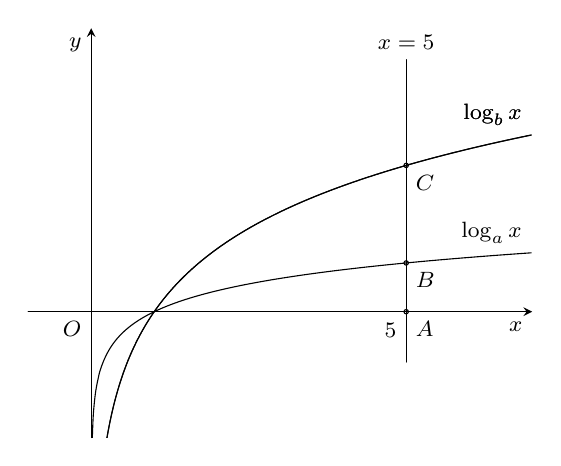
\begin{tikzpicture}[scale=0.8, font=\footnotesize, line join=round, line cap=round, >=stealth]
			\tikzset{label style/.style={font=\footnotesize}}
			\def \xmin{-1}
			\def \xmax{7}
			\def \ymin{-2}
			\def \ymax{4.5}
			\def \hamso{sin(\x r)}
			\draw[->] (\xmin,0)--(\xmax,0) node[below left] {$x$};
			\draw[->] (0,\ymin)--(0,\ymax) node[below left] {$y$};
			\draw (0,0) node [below left] {$O$};
			\foreach \x in {5}
			\draw[thin] (\x,1pt)--(\x,-1pt) node [below left] {$\x$};
			\begin{scope}
				\clip (\xmin+0.01,\ymin+0.01) rectangle (\xmax-0.01,\ymax-0.01);
				\draw[samples=350,domain=0.01:\xmax-0.01,smooth,variable=\x] plot (\x,{ln(\x)/ln(2)}) node[above left]{$\log_{b} x$};
				\draw[samples=350,domain=0.01:\xmax-0.01,smooth,variable=\x] plot (\x,{ln(\x)/ln(8)}) node[above left]{$\log_{a} x$};
				\draw[samples=350,domain=0.01:\xmax-0.01,smooth,variable=\x] plot (\x,{ln(\x)/ln(2)}) node[above left]{$\log_{b} x$};
				\draw(5,-0.8)--(5,4) node[above]{$x=5$};
				\draw(5.,0.) circle (1.0pt) node[below right]{$A$};
				\draw(5.,{ln(5)/ln(8)}) circle (1.0pt) node[below right]{$B$};
				\draw(5.,{ln(5)/ln(2)}) circle (1.0pt) node[below right]{$C$};
			\end{scope}
	\end{tikzpicture}}
	\loigiai{
		Ta có $A(5; 0)$, $B\left(5;\log_{a}5\right)$, $C\left(5;\log_{b}5\right)$.\\
		Do đó	
		\begin{eqnarray*}
			&CB=2AB &\Leftrightarrow \log_{b}5-\log_{a}5=2\log_{a}5\\
			&&\Leftrightarrow \log_{b}5=3\log_{a}5\\
			&&\Leftrightarrow \log_{5}a=3\log_{5}b\\
			&&\Leftrightarrow a=b^3.
		\end{eqnarray*}
		Vậy $m=1$, $n=3$ nên $m^2+n^2=10$.
	}
\end{ex}

% #4266 | Archive/SP-4Phan-Dot3/Data/CTST_1-OTHK2_De02.tex | mã gốc 1D6V4-6
\begin{ex}%[1D6V4-6]
	Một loại chất phóng xạ có chu kỳ bán rã là $T$ (giờ). Biết rằng lượng chất phóng xạ còn lại sau thời gian $t$ (giờ) tính từ thời điểm ban đầu là $Q=Q_0\cdot 2^{-\tfrac{t}{T}}$, trong đó $_0$ là lượng chất phóng xạ ban đầu. Nếu ban đầu có $100$ gam chất phóng xạ và sau $3$ giờ còn lại $80$ gam. Sau bao lâu thì lượng chất phóng xạ còn lại chỉ bằng $10\%$ lượng ban đầu? (Kết quả làm tròn đến hằng đơn vị).
	\shortans{30}
	\loigiai{
		Theo bài ra ta có 
		$Q_0=100$ gam, $t=3$ giờ, $Q=80$ gam (sau $3$ giờ).\\
		Ta có $80=100\cdot 2^{-\frac{3}{T}}\Leftrightarrow  2^{-\frac{3}{T}}=0{,}8\Leftrightarrow -\dfrac{3}{T}=\log_2 0{,}8\Leftrightarrow T=-\dfrac{3}{\log_2(0{,}8)}\approx 9{,}31$ giờ.\\
		Ta có $Q_0=100$ gam, $t=3$ giờ, $Q=10\%$ của $100$ gam $=10$ gam.\\
		Ta có $10=100\cdot 2^{-\frac{t}{9{,}31}}\Rightarrow t=-9{,}31\cdot \log_2 (0{,}1)\approx 30$ giờ.\\
		Vậy sau khoảng $30$ giờ thì lượng chất phóng xạ còn lại chỉ bằng $10\%$ lượng ban đầu.
	}	
\end{ex}

% #4281 | Archive/SP-4Phan-Dot3/Data/CTST_1-OTHK2_De03.tex | mã gốc 1D6N4-2
\begin{ex}%[1D6N4-2]
	Giải các phương trình sau $3^{x-1}=27$.
	\loigiai{
		Ta có $3^{x-1}=27\Leftrightarrow3^{x-1}=3^3\Leftrightarrow x-1=3\Leftrightarrow x=4$.
	}
\end{ex}

% #4287 | Archive/SP-4Phan-Dot3/Data/CD_1_OTGK2_De02.tex | mã gốc 1D6V3-5
\begin{ex}%[1D6V3-5]
	Giả sử dân số của một thành phố tăng trưởng theo mô hình hàm số mũ với tỷ lệ tăng trưởng hàng năm là $2\%$, được biểu diễn bằng công thức
	$$P(t)=P_0\cdot \mathrm{e}^{0{,}02t}$$
	Trong đó
	\begin{itemize}
		\item $P(t)$ là dân số sau $t$ năm.
		\item $P_0$ là dân số ban đầu.
	\end{itemize}
	Cho dân số ở thành phố này là $4{,}5$ triệu dân, để dân số ở thành phố này đạt mốc $5$ triệu dân thì cần ít nhất bao nhiêu tháng (số nguyên) để đạt được mốc này?
	\shortans[oly]{$64$}
	\loigiai{
		Thời gian để dân số này đạt mốc $5$ triệu dân tính theo năm là
		$$5=4{,}5 \cdot\mathrm{e}^{0{,}02t}
		\Rightarrow t\approx 5{,}268 \text{ (năm).}$$
		Thời gian để dân số này đạt mốc $5$ triệu dân tính theo tháng là
		$$5{,}268\cdot12=63{,}216 \text{ (tháng).}$$
		Vậy cần ít nhất $64$ tháng để thành phố đạt được mốc $5$ triệu dân.
	}
\end{ex}

% #4289 | Archive/SP-4Phan-Dot3/Data/CD_1_OTGK2_De02.tex | mã gốc 1D6V2-2
\begin{ex}%[1D6V2-2]
	Cường độ âm thanh $L$ (đơn vị: decibel, dB) được tính bằng công thức \break $L=10\cdot\log\left(\dfrac{I}{I_0}\right)$.	Trong đó
	\begin{itemize}
		\item $I$ là mức cường độ âm thanh đo được (đơn vị: W/m$^2$).
		\item $I_0$ là mức cường độ âm thanh chuẩn (thường là $10^{-12}$ W/m$^2$).
	\end{itemize}
	Giả sử bạn đứng gần một nguồn âm thanh và đo được cường độ âm thanh là $80$ dB. Nếu bạn di chuyển xa hơn nguồn âm thanh làm mức cường độ âm thanh giảm đi $10$ lần, hãy tính cường độ âm thanh mới mà bạn nghe được.
	\loigiai{
		Mức cường độ âm thanh ban đầu là
		\begin{eqnarray*}
			L_1&=&10\cdot\log \left( \dfrac{I_1}{I_0} \right) \\
			80&=&10\cdot\log \left( \dfrac{I_1}{10^{-12}} \right)\\
			I_1&=&10^{-4}  \text{ W/m}^2.
		\end{eqnarray*}
		Khi đó cường độ âm thanh mới sẽ là
		\begin{eqnarray*}
			L_2&=&10\cdot\log \left( \dfrac{I_2}{I_0} \right) \\
			L_2&=&10\cdot\log \left( \dfrac{\dfrac{I_1}{10}}{10^{-12}} \right) \\
			L_2&=&10\cdot\log \left( \dfrac{\dfrac{10^{-4}}{10}}{10^{-12}} \right) \\
			L_2&=&70 \text{ dB}.
		\end{eqnarray*}
	}
\end{ex}

% #4300 | Archive/SP-4Phan-Dot3/Data/CD_1_OTHK2_De04.tex | mã gốc 1D6V2-5
\begin{ex}%[1D6V2-5]
	Một người gửi $150$ triệu đồng vào một ngân hàng theo thể thức lãi xuất kép với lãi xuất cố định là $8{,}4\%$/năm. Nếu theo kì hạn một năm thì sau ít nhất bao nhiêu năm, người đó thu được cả vốn và tiền lãi hơn $200$ triệu đồng?
	\shortans[]{$4$}
	\loigiai
	{
	Số tiền người đó thu được sau $n$ năm là $S=150\cdot{\left(1+\dfrac{8{,}4}{100}\right)^n}$ (triệu).\\
	Ta có
		\begin{eqnarray*}
			&  S>200 &\Leftrightarrow 150 \cdot{\left(1+\dfrac{8{,}4}{100}\right)^n}>200\\
			& &\Leftrightarrow {\left(1+\dfrac{8{,}4}{100}\right)^n}>\dfrac{4}{3}\\
			& &\Leftrightarrow n\log 1{,}084>\log \dfrac{4}{3}\Leftrightarrow n>3{,}57.
		\end{eqnarray*}
	Vậy phải sau ít nhất $4$ năm thì người đó thu được cả vốn và tiền lãi hơn $200$ triệu đồng.
}
\end{ex}

% #4302 | Archive/SP-4Phan-Dot3/Data/CD_1_OTHK2_De04.tex | mã gốc 1D6H4-3
\begin{bt}%[1D6H4-3]
	Giải bất phương trình $\log_4 (x+7)>\log_2 (x+1)$.
	\loigiai{Điều kiện $ x>-1 $.\\
		Ta có
		\allowdisplaybreaks
		\begin{eqnarray*}
			& & \log_4 (x+7)>\log_2 (x+1)\\
			&\Leftrightarrow &\dfrac{1}{2}\log_2 (x+7)>\log_2 (x+1)\\
			&\Leftrightarrow & \log_2 (x+7)>2\log_2 (x+1)\\
			& \Leftrightarrow &x+7>(x+1)^2\\
			&\Leftrightarrow & x^2+x-6<0\Leftrightarrow -3<x<2.
		\end{eqnarray*}
		Vậy tập nghiệm của bất phương trình $S=(-1 ; 2)$.
	}
\end{bt}

% #4308 | Archive/SP-4Phan-Dot3/Data/KNTT_1-OTGK2_De04.tex | mã gốc 1D6V3-5
\begin{ex}%[1D6V3-5]
	Khối lượng vi khuẩn của một mẻ nuôi cấy sau $ t$ giờ kể từ thời điểm ban đầu được cho bởi công thức $M(t)=50\cdot 1{,}06^t$ (g). Khối lượng vi khuẩn sau $24$ giờ gấp bao nhiêu lần số lượng vi khuẩn ban đầu? Kết quả làm tròn đến hàng đơn vị.
	\shortans{$4$}
	\loigiai{
		Ta có  $\dfrac{M(24)}{M(0)}=\dfrac{50\cdot 1{,}06^{24}}{50}\approx 4$.
	}
\end{ex}

% #4309 | Archive/SP-4Phan-Dot3/Data/KNTT_1-OTGK2_De04.tex | mã gốc 1D6V4-6
\begin{ex}%[1D6V4-6]
	Dân số ở một địa phương được ước tính theo công thức $S=A\cdot e^{rt}$, trong đó $A$ không đổi là dân số của năm 2023, $S$ là dân số sau $t$ năm, $r$ là tỉ lệ tăng dân số hằng năm. Hỏi đến năm nào thì dân số ở địa phương đó sẽ đạt gấp đôi dân số năm 2023? Biết $r=1,13\% /$ năm.
	\loigiai{
		Dân số đạt gấp đôi nghĩa là $S=2A$, ta có
		\[2A=A\cdot \mathrm{e}^{1{,}13\%\cdot t} \Leftrightarrow \mathrm{e}^{1{,}13\%\cdot t}=2\Leftrightarrow 1{,}13\%\cdot t=\ln_\mathrm{e} 2\Leftrightarrow t=\dfrac{\ln 2}{1{,}13\%} \approx 61{,}34 \; (do\; \mathrm{e} > 1 \;).\;
		\]
		Vậy sau $62$ năm tức đến năm $2085$ thì dân số ở địa phương đó sẽ gấp đôi dân số năm $2023$.
	}
\end{ex}

% #4313 | Archive/SP-4Phan-Dot3/Data/CTST_1-OTGK2_De05.tex | mã gốc 1D6H5-1
\begin{ex}%[1D6H5-1]
	Giải phương trình $\log_2^2(x+1)-6\log_2\sqrt{x+1}+2=0$.
	\loigiai{
		Điều kiện xác định $x+1>0\Leftrightarrow x >-1$.\\
		Ta có $\log_2^2(x+1)-6\log_2\sqrt{x+1}+2=0\Leftrightarrow \log_2^2(x+1)-3\log_2(x+1)+2=0$.\\
			Đặt $t=\log_2(x+1)$ thì phương trình trở thành $t^2-3t+2=0$.\\
		Ta có $t^2-3t+2=0\Leftrightarrow \hoac{& t=1 \\ & t=2.}$\\
			Với $t=1\Leftrightarrow \log_2(x+1)=1\Leftrightarrow x=1$. (thỏa điều kiện)\\
			Với $t=2\Leftrightarrow \log_2(x+1)=2\Leftrightarrow x=3$. (thỏa điều kiện)\\
			Vậy phương trình có hai nghiệm nguyên dương là $x=1$ và $x=3$.
	}
\end{ex}

% #4319 | Archive/SP-4Phan-Dot3/Data/CTST_1-OTGK2_De04.tex | mã gốc 1D6V4-6
\begin{ex}%[Nguyễn Tuấn, sáng tác đề GHK2 toán 11]%[1D6V4-6]
	Độ pH của một dung dịch được tính theo công thức $\mathrm{pH}=-\log x$,  trong đó $x$ 
	là nồng độ ion $\mathrm{H}^+$ của dung dịch đó tính bằng mol/L. Biết rằng độ pH của dung dịch $A$ lớn hơn độ
	pH của dung dịch $B$ là $0{,}6$. Dung dịch $B$ có nồng độ ion $\mathrm{H}^+$ gấp bao nhiêu lần nồng độ ion $\mathrm{H}^+$ của 
	dung dịch $A$?
	\shortans{4}
	\loigiai{Gọi $x_A$ là nồng độ ion của dung dịch $A$, $x_B$ là nồng độ ion của dung dịch $B$.\\
		Ta có $-\log x_A-(-\log x_B)=0{,}6\Rightarrow \log x_B-\log x_A=0{,}6\Rightarrow \log \dfrac{x_B}{x_A}=0{,}6$.\\
		Suy ra ta có $\dfrac{x_B}{x_A}=10^{0,6}\approx 4$ hay $x_B=4x_A$.\\
		Vậy dung dịch $B$ có nồng độ ion $\mathrm{H}^+$ gấp $4$ lần nồng độ ion $\mathrm{H}^+$ của 
		dung dịch $A$}
\end{ex}

% #4325 | Archive/SP-4Phan-Dot3/Data/KNTT_1-OTGK2_De05.tex | mã gốc 1D6V4-6
\begin{ex}%[1D6V4-6]
	Năm $2\,022$, một hãng công nghệ có $30$ triệu người dùng phần mềm của họ. Hãng đặt kế hoạch, trong $3$ năm tiếp theo, mỗi năm số lượng người dùng phần mềm tăng $8\%$ so với năm trước và từ năm thứ $4$ trở đi, số lượng người dùng phần mềm sẽ tăng $5\%$ so với năm trước đó. Theo kế hoạch đó, hỏi bắt đầu từ năm nào số lượng người dùng phần mềm của hãng sẽ vượt quá $50$ triệu người?
	\shortans[oly]{2031}
	\loigiai{
		Số lượng người dùng phần mềm của công ty sau $3$ năm
		$$T_1=30\cdot \left(1+\dfrac{8}{100} \right)^3\approx 37{,}79.$$
		Số lượng người dùng phần mềm của công ty sau $n$ năm tiếp theo $$T_2=37{,}79\cdot \left(1+\dfrac{5}{100} \right)^n.$$
		Để người dùng vượt quá $50$ triệu người thì\\ 
		$$37{,}79\cdot \left(1+\dfrac{5}{100} \right)^n > 50\Leftrightarrow n > 5.$$
		Mà $n\in \mathbb{N}$ nên $n=6$.\\
		Suy ra cần ít nhất $3+6=9$ năm.\\
		Vậy bắt đầu từ năm $2\,022+9=2\,031$ thì số lượng người dùng phần mềm của hãng sẽ vượt quá $50$ triệu người
	}
\end{ex}

% #4326 | Archive/SP-4Phan-Dot3/Data/KNTT_1-OTGK2_De05.tex | mã gốc 1D6V4-6
\begin{ex}%[1D6V4-6]
	Độ pH của một dung dịch được tính theo công thức $pH=-\log x$,  trong đó $x$ 
	là nồng độ ion $H^+$ của dung dịch đó tính bằng mol/L. Biết rằng độ $pH$ của dung dịch $A$ lớn hơn độ $pH$ của dung dịch $B$ là $0{,}6$. Dung dịch $B$ có nồng độ ion $H^+$ gấp bao nhiêu lần nồng độ ion $H^+$ của dung dịch $A$ (làm tròn kết quả đến chữ số hàng đơn vị)?
	\par \shortans[oly]{4}
	\loigiai{
		Gọi $x_A$ là nồng độ ion của dung dịch $A$, $x_B$ là nồng độ ion của dung dịch $B$.\\
		Ta có \begin{eqnarray*}
			&&-\log x_A-(-\log x_B)=0,6\\
			&\Rightarrow& \log x_B-\log x_A=0,6\\
			&\Rightarrow& \log \dfrac{x_B}{x_A}=0,6\\
			&\Rightarrow&\dfrac{x_B}{x_A}=10^{0,6}\approx 4\\
			&\Rightarrow& x_B=4x_A.
		\end{eqnarray*}				
		Vậy dung dịch $B$ có nồng độ ion $H^+$ gấp $4$ lần nồng độ ion $H^+$ của dung dịch $A$.
	} 
\end{ex}

% #4329 | Archive/SP-4Phan-Dot3/Data/KNTT_1-OTGK2_De05.tex | mã gốc 1D6V4-4
\begin{ex}%[1D6V4-4]%%Tự luận 1
		Giải phương trình $9^{x+1}-13\cdot 6^x+4^{x+1}=0$.
	\loigiai{
			Ta có \allowdisplaybreaks
			\begin{eqnarray*}
				&&9^{x+1}-13\cdot 6^x+4^{x+1}=0\\
				&\Leftrightarrow& 9\cdot 9^x-13\cdot 6^x+4\cdot 4^x=0\\
				&\Leftrightarrow& 9\cdot \dfrac{9^x}{4^x}-13\cdot \dfrac{6^x}{4^x}+4=0\\
				&\Leftrightarrow& 9\cdot\left(\dfrac{3}{2} \right)^{2x}-13\cdot\left(\dfrac{3}{2} \right)^x+4=0\\
				&\Leftrightarrow& \hoac{&\left(\dfrac{3}{2} \right)^x=1 \\
				&\left(\dfrac{3}{2} \right)^x=\dfrac{4}{9}}\\
				&\Leftrightarrow& \hoac{&x=0\\&x=-2.}	
			\end{eqnarray*}			
		}
\end{ex}

% #4330 | Archive/SP-4Phan-Dot3/Data/KNTT_1-OTGK2_De05.tex | mã gốc 1D6V3-5
\begin{ex}%[1D6V3-5]%%Tự luận 2
	Nếu $D_0$ là chênh lệch nhiệt độ ban đầu giữa một vật $M$ và các vật xung quanh, và nếu các vật xung quanh có nhiệt độ $T_S$, thì nhiệt độ của vật $M$ tại thời điểm $t$ được mô hình hóa bởi hàm số $T(t)=T_S+D_0 \cdot \mathrm{e}^{-kt}$ (trong đó $k$ là hằng số dương phụ thuộc vào vật $M$). Một con gà tây nướng được lấy từ lò nướng khi nhiệt độ của nó đã đạt đến $195^\circ$F và được đặt trên một bàn trong một căn phòng có nhiệt độ là $65^\circ$F. Nếu nhiệt độ của gà tây là $150^\circ$F sau nửa giờ, nhiệt độ của nó sau $60$ phút là bao nhiêu độ F (làm tròn kết quả đến chữ số hàng đơn vị)? 
	\loigiai{
		Ta có $T_S=65$ và độ chênh lệch nhiệt độ là $D_0=195-65=130^\circ$F.\\
		Sau nửa giờ $(t=0{,}5)$ thì nhiệt độ của gà là $T=150^\circ$F.\\
		Từ hàm số $T(t)=T_S+D_0 \cdot \mathrm{e}^{-kt}$, ta có 
		$$150=65+130\cdot \mathrm{e}^{-k(0{,}5)} \Leftrightarrow \mathrm{e}^{-k}=\left(\dfrac{17}{26} \right)^2.$$
		Vậy $T(t)=65+130\cdot \left(\dfrac{17}{26} \right)^{2t}$.\\
		Suy ra nhiệt độ của gà sau $60$ phút suy ra $t=1$ (giờ) là 
		$$65+130\cdot \left(\dfrac{17}{26} \right)^{2\cdot 1} \approx 121^\circ \text {F}.$$
	}
\end{ex}

% #4335 | Archive/SP-4Phan-Dot3/Data/CD_1_OTHK2_De05.tex | mã gốc 1D6V4-6
\begin{ex}%[1D6V4-6]
	Dân số của Việt Nam năm $2009$ là $85\,846\,997$ người và năm $2019$ là $96\,208\,984$ người. Sử dụng mô hình tăng trưởng mũ $S(n)=A \cdot \mathrm{e}^{n r}$ (trong đó $A$ là dân số của năm $2009$, $S$ là dân số sau $n$ năm kể từ năm $2009$, $r$ là tỉ lệ tăng dân số hàng năm) để dự doán xem vào năm bao nhiêu dân số Việt Nam vượt ngưỡng $150$ triệu người.
	\shortans[oly]{2009}
	\loigiai{
		Ta có dân số của Việt Nam vào năm $2019$ là $S(10)$ nên $$96\,208\,984=85\,846\,997\cdot \mathrm{e}^{10 r}\Rightarrow r\approx 0{,}0114.$$
		Dân số Việt Nam vượt ngưỡng $150$ triệu người khi 
		\begin{eqnarray*}
			&&S(n)>150\,000\,000\\
			&\Rightarrow&  85\,846\,997\cdot \mathrm{e}^{n\cdot 0{,}0114}>150\,000\,000\\
			&\Rightarrow&  \mathrm{e}^{n\cdot 0{,}0114}>\dfrac{150\,000\,000}{85\,846\,997}\\
			&\Rightarrow& n>48{,}96.
		\end{eqnarray*}
		Vậy vào khoảng năm $2009+49=2068$ thì dân số Việt Nam vượt ngưỡng $150$ triệu người.
	}
\end{ex}

% #4338 | Archive/SP-4Phan-Dot3/Data/CD_1_OTHK2_De05.tex | mã gốc 1D6H4-4
\begin{ex}%[1D6H4-4]
	Giải phương trình $\log _{\frac{1}{5}}\left(x^2-6 x+18\right)+2 \log _5(x-4)=0$.
	\loigiai{
		Điều kiện xác định $\heva{&x^2-6 x+18>0\\&x-4>0}\Leftrightarrow x>4$.\\
		Khi đó 
		\begin{eqnarray*}
			&&\log _{\frac{1}{5}}\left(x^2-6 x+18\right)+2 \log _5(x-4)=0\\
			&\Leftrightarrow& \log_5 (x-4)^2=\log_5 \left(x^2-6 x+18\right)\\
			&\Leftrightarrow& x^2-8x+16=x^2-6 x+18\\
			&\Leftrightarrow& x=-1.~ \text{(loại)}
		\end{eqnarray*}
		Vậy phương trình vô nghiệm.
	}
\end{ex}

% #4341 | Archive/SP-4Phan-Dot3/Data/CTST_1-OTGK2_De06.tex | mã gốc 1D6H2-3
\begin{ex}%[1D6H2-3] 
Trong điện hóa học, phương trình Nernst là một mối quan hệ nhiệt động hóa học cho phép tính toán thế khử của phản ứng (phản ứng nửa pin hoặc toàn pin) từ thế điện cực chuẩn, nhiệt độ tuyệt đối, số electron tham gia vào phản ứng oxid hóa khử và hoạt động (thường xấp xỉ theo nồng độ) của các tiểu phân trải qua quá trình khử và oxy hóa tương ứng.\\
Phương trình Nernst có dạng tổng quát như sau
$E^o = E + \dfrac{RT}{nF}.\left(\ln{\dfrac{C_{ox}}{C_{red}}}\right)$.\\
Cho biết $F = 96485;
R = 8{,}314; T=298$\\
Các đại lượng còn lại giữ nguyên kí hiệu. Khi đó
    \choiceTF
 {Kí hiệu $\ln{\dfrac{C_{ox}}{C_{red}}}$ là logarit cơ số $10$ của $\dfrac{C_{ox}}{C_{red}}$ }
{\True Phương trình Nernst với số liệu trên có thể biến đổi thành một phương trình đơn giản hơn là
$E^o = E + \dfrac{0,0592}{n}\cdot\log{\dfrac{C_{ox}}{C_{red}}}$}
{\True Với $\dfrac{C_{ox}}{C_{red}} = 1 $ thì $E^o = E$}
{Phương trình Nernst có thể viết thành $E^o = E + \dfrac{RT}{nF}\cdot\left(\ln{C_{ox}} + \ln{C_{red}}\right)$}
\loigiai{\begin{itemchoice} 
			\itemch Sai.
   $\ln$ là kí hiệu của logarit cơ số $e$ (logarit tự nhiên) của $\dfrac{C_{ox}}{C_{red}}$\\
                \itemch Đúng. Ta có 
                $E^o = E + \dfrac{RT}{nF}\cdot\left(\ln{\dfrac{C_{ox}}{C_{red}}}\right)\\
                E^o = E + \dfrac{8{,}314\cdot298}{n\cdot96485}\cdot\ln{10}\cdot\log{\dfrac{C_{ox}}{C_{red}}}\\
                E^o = E + \dfrac{0{,}0592}{n}\cdot \left(\log{\dfrac{C_{ox}}{C_{red}}}\right)$.\\
			\itemch Đúng. Ta có $\ln{1} = 0 \Rightarrow E^o = E + \dfrac{RT}{nF}\cdot 0 \Rightarrow E^o = E$.\\
                \itemch Sai. Ta có $\log{_a}{\dfrac{c}{d}} = \log{_a}{c} - \log{_a}{d}
                \Rightarrow E^o = E + \dfrac{RT}{nF}\cdot(\ln{C_{ox}} - \ln{C_{red}})$.
   \end{itemchoice}
  }
\end{ex}

% #4343 | Archive/SP-4Phan-Dot3/Data/CTST_1-OTGK2_De06.tex | mã gốc 1D6H4-6
\begin{ex}%[1D6H4-6] 
	Số lượng loại vi khuẩn $A$ trong một phòng thí nghiệm được tính theo công thức $s(t)=s(0)\cdot 2^t$, trong đó $s(0)$ là số lượng vi khuẩn $A$ lúc ban đầu, $s(t)$ là số lượng vi khuẩn $A$ có sau $t$ phút. Biết sau $3$ phút thì số vi khuẩn $A$ là $625$ nghìn con. Hỏi sau bao lâu kể từ lúc ban đầu, số lượng loại vi khuẩn $A$ là $20$ triệu con.
	\shortans[0]{8}
	\loigiai{
		Theo giả thiết ta có: $s(3)=625\,000\Leftrightarrow s(0)\cdot 2^3=625\,000\Leftrightarrow s(0)=78\,125$.\\
		Số lượng loại vi khuẩn $A$ là 20 triệu con khi\\
		$s(t)=20\,000\,000\Leftrightarrow s(0)\cdot 2^t=20\,000\,000
		\Leftrightarrow {2^t}=\dfrac{20\,000\,000}{s(0)}=\dfrac{20\,000\,000}{78\,125}=256
		\Leftrightarrow t=8$.\\
		Vậy sau $8$ phút thì số lượng vi khuẩn $A$ là $20$ triệu con.
	}
\end{ex}

% #4344 | Archive/SP-4Phan-Dot3/Data/CTST_1-OTGK2_De06.tex | mã gốc 1D6H4-6
\begin{ex}%[1D6H4-6] 
 Nếu khối lượng carbon-14 trong cơ thể sinh vật lúc chết là $M_0(\mathrm{~g})$ thì khối lượng carbon-14 còn lại (tính theo gam) sau $t$ năm được tính theo công thức $M(t)=M_0\left(\frac{1}{2}\right)^{\frac{t}{T}}(\mathrm{~g})$, trong đó $T=5730$ (năm) là chu kì bán rã của carbon-14. Nghiên cứu hoá thạch của một sinh vật, người ta xác định được khối lượng carbon-14 hiện có trong hoá thạch là $5 \cdot 10^{-13} \mathrm{~g}$. Nhờ biết tỉ lệ khối lượng của carbon- 14 so với carbon- 12 trong cơ thể sinh vật sống, người ta xác định được khối lượng carbon-14 trong cơ thể lúc sinh vật chết là $M_0=1,2 \cdot 10^{-12}(\mathrm{~g})$. Sinh vật này sống cách đây bao nhiêu năm? (Làm tròn kết quả đến hàng trăm.)
\shortans[0]{7200}
\loigiai{
Gọi $t$ là thời gian từ lúc sinh vật chết đến nay. Ta có
$$
\begin{aligned}
	5 \cdot 10^{-13}=1,2 \cdot 10^{-12} \cdot\left(\frac{1}{2}\right)^{\frac{t}{T}} & \Leftrightarrow\left(\frac{1}{2}\right)^{\frac{t}{T}}=\frac{5}{12} \Leftrightarrow \frac{t}{T}=\log _{\frac{1}{2}} \frac{5}{12} \\
	& \Leftrightarrow t=T \log _{\frac{1}{2}} \frac{5}{12}=-5\,730 \cdot \log _2 \frac{5}{12} \approx 7\,237 \approx 7\,200
\end{aligned}
$$
Vậy sinh vật này sống cách đây khoảng $7\,200$ năm.
}	
\end{ex}

% #4348 | Archive/SP-4Phan-Dot3/Data/CTST_1-OTGK2_De06.tex | mã gốc 1D6V3-5
\begin{ex}%[1D6V3-5]
	Theo số liệu thực tế, dân số thế giới năm $1950$ là $2560$ triệu người, còn năm $1980$ là $3040$ triệu người. Người ta dự đoán dân số thế giới phụ thuộc vào thời gian $t$ theo hàm số mũ $P\left( t \right) = a\cdot{e^{bt}}$ với $a, b$  là hằng số và độ biến thiên của $P(t)$ theo thời gian tỷ lệ thuận với $P\left( t \right)$. Hãy dự đoán dân số thế giới vào năm 2030 (làm tròn đến triệu người).
%	\shortans[0]{4048}
	\loigiai{Dân số thế giới tại thời điểm $1950$ là $P_{1950} = a\cdot e^{b\cdot 1950} = 2560.$\\  
		Dân số thế giới tại thời điểm 1980 là $P_{1980} = a\cdot{e^{b\cdot 1980}} = 3040$.\\
		Ta có $\dfrac{a\cdot e^{b\cdot 1980}}{a\cdot e^{b\cdot 1950}} = \dfrac{3040}{2560} \Leftrightarrow e^{30b} = \dfrac{19}{16}$.\\
		Lấy lô ga rit cơ số $e$ hai vế ta được $\ln{e^{30b}} = \ln \dfrac{19}{16} \Leftrightarrow 30b = \ln \dfrac{19}{16} \Rightarrow b = \dfrac{1}{30}\cdot\ln \dfrac{19}{16}$.\\
		Suy ra $a\cdot e^{65\cdot \ln \tfrac{19}{16}} = 2560 \Rightarrow a = \dfrac{2560}{e^{65\cdot\ln \tfrac{19}{16}}}$.\\
		Vậy dân số thế giới năm $2030$ là $P_{2030} = a\cdot{e^{b\cdot 2030}} \approx 4048$ triệu người.
	}
\end{ex}

% #4349 | Archive/SP-4Phan-Dot3/Data/CTST_1-OTGK2_De06.tex | mã gốc 1D6V4-6
\begin{ex}%[1D6V4-6]
	Trong năm $2019$, diện tích rừng trồng mới của tỉnh $A$ là $800$ ha. Giả sử diện tích rừng trồng mới của tỉnh $A$ mỗi năm tiếp theo đều tăng   $6\%$ so với diện tích rừng trồng mới của năm liền trước. Kể từ sau năm  $2019$, năm nào là năm đầu tiên tỉnh $A$ có diện tích rừng trồng mới trong năm đó đạt trên  $1\,400$ ha?
%	\shortans[0]{$2029$}
	\loigiai{Trong năm  $2019$, diện tích rừng trồng mới của tỉnh $A$ là $800$ ha. Giả sử diện tích rừng trồng mới của tỉnh $A$ mỗi năm tiếp theo đều tăng  $6\%$ so với diện tích rừng trồng mới của năm liền trước nên sau $n$ (năm), diện tích rừng trồng mới của tỉnh $A$ là $800.\left(1 + 6\%  \right)^n$ với  $n\in \mathbb{N}$.\\
		Ta có $800\cdot{\left( {1 + 6\% } \right)^n} \ge 1\,400 \Leftrightarrow 1{,}06^n \ge \dfrac{7}{4} \Leftrightarrow n \ge {\log _{1{,}06}}\frac{7}{4} \approx 9{,}60402$.\\
		Vì  $n\in \mathbb{N}$ nên giá trị nhỏ nhất thỏa mãn là  $n=10$. \\
		Vậy kể từ sau năm  $2019$, năm đầu tiên tỉnh $A$ có diện tích rừng trồng mới trong năm đó đạt trên $1\,400$ ha là năm $2029$.
	}
\end{ex}

% #4351 | Archive/SP-4Phan-Dot3/Data/CD_1_OTHK2_De06.tex | mã gốc 1D6V4-6
\begin{ex}%[Làm đề GHK, HK, 4 phần - 2025]%[Huỳnh Xuân Tín]%[1D6V4-6]
	Người ta dùng thuốc để khử khuẩn cho một thùng nước. Biết rằng nếu lúc đầu mỗi mililít nước chứa $P_{0}$ vi khuẩn thì sau $t$ giờ (kể từ khi cho thuốc vào thùng), số lượng vi khuẩn trong mỗi mililít nước là $P=P_0 \cdot 10^{-\alpha t}$, với $\alpha$ là một hằng số dương nào đó. Biết rằng ban đầu mỗi mililít nước có $9\,000$ vi khuẩn và sau $2$ giờ, số lượng vi khuẩn trong mỗi mililit nước là $6\,000$. Sau thời gian bao lâu thì số lượng vi khuẩn trong mỗi mililit nước trong thùng ít hơn hoặc bằng $1\,000$ (làm tròn đến hàng phần mười)?
	\shortans[]{$10{,}8$}
	\loigiai{
		Ta có $6\,000=9\,000\cdot 10^{-2\alpha} \Rightarrow \alpha=-\dfrac{1}{2} \log \dfrac{2}{3}=\dfrac{1}{2} \log \dfrac{3}{2}$.\\
		\allowdisplaybreaks
		\begin{eqnarray*}
			9\,000 \cdot 10^{-\alpha t} \leq 1\,000 
			&\Leftrightarrow & 10^{-\alpha t} \leq \dfrac{1}{9} \\
			&\Leftrightarrow &-\alpha t \leq \log \dfrac{1}{9}	\\
			&\Leftrightarrow &t \geq-\dfrac{2}{\alpha} \log \dfrac{1}{3}=-\dfrac{2}{\dfrac{1}{2} \log \dfrac{3}{2}} \cdot \log \dfrac{1}{3}=\dfrac{4 \log 3}{\log \dfrac{3}{2}} \approx 10{,}8 \ \text{(giờ).}
		\end{eqnarray*}
	}
\end{ex}

% #4355 | Archive/SP-4Phan-Dot3/Data/CD_1_OTHK2_De06.tex | mã gốc 1D6H4-5
\begin{ex}%[Làm đề GHK, HK, 4 phần - 2025]%[Huỳnh Xuân Tín]%[1D6H4-5]
	Giải bất phương trình $\log_{0{,}3}{(x+1)}\leq\log_{0{,}3}{(2x-1)}$.
	\loigiai{
		Điều kiện: $x>\dfrac{1}{2}$.\\
		Vì cơ số $0{,}3<1$ nên bất phương trình trở thành $x+1\geq2x-1$, từ đó tìm được $x\leq 2$.\\
		Kết hợp điều kiện, ta được nghiệm của bất phương trình đã cho là $\dfrac{1}{2}<x\leq2$.
	}
\end{ex}

% #4361 | Archive/SP-4Phan-Dot3/Data/CD_1_OTHK2_De02.tex | mã gốc 1D6V4-6
\begin{ex}%[1D6V4-6]
	Một người gửi $75$ triệu đồng vào một ngân hàng với lãi suất $6{,}5$\%/năm. Biết rằng nếu không rút tiền ra khỏi ngân hàng thì cứ sau mỗi năm số tiền lãi sẽ được nhập vào gốc để tính lãi cho năm tiếp theo. Hỏi sau ít nhất bao nhiêu năm người đó nhận được số tiền nhiều hơn $110$ triệu đồng bao gồm cả gốc và lãi? Giả định suốt trong thời gian gửi, lãi suất không đổi và người đó không rút tiền ra.
	
	\shortans[]{$7$}
	\loigiai{
		Gọi $n$ là số năm cần tìm, điều kiện $n\in \mathbb{N}^*$.\\
		Khi đó $n$ là nghiệm nguyên dương nhỏ nhất của bất phương trình
		\[75\cdot (1+0{,}065)^n>110\Leftrightarrow 1{,}065^n>\dfrac{22}{15}\Leftrightarrow n>\log_{1{,}065}\dfrac{22}{15}=6{,}08167.\]
		Vậy giá trị của $n$ thỏa đề bài là $n=7$.
	}
\end{ex}

% #4369 | Archive/SP-4Phan-Dot3/Data/KNTT_1-OTGK2_De02.tex | mã gốc 1D6V4-6
\begin{ex}%[1D6V4-6]
	Một điện thoại đang nạp pin, dung lượng pin nạp được tính theo công thức $Q(t)=Q_0\cdot (1-\mathrm{e}^{-t\sqrt2})$ với $t$ là khoảng thời gian tính bằng giờ và $Q_0$ là dung lượng nạp tối đa (pin đầy). Hãy tính thời gian nạp pin của điện thoại tính từ lúc cạn hết pin cho đến khi điện thoại đạt được $95\%$ dung lượng pin tối đa (kết quả được làm tròn đến hàng phần trăm).
	\shortans{$2{,}12$}
	\loigiai{
		Ta có phương trình
		\begin{eqnarray*}
			&  &95\%Q_0=Q_0(1-\mathrm{e}^{-t\sqrt2})\\
			&\Leftrightarrow &\mathrm{e}^{-t\sqrt2}=1-0,95\\
			&\Leftrightarrow &\mathrm{e}^{-t\sqrt2}=0,05\\
			&\Leftrightarrow & -t\sqrt2=\ln0{,}05\\
			&\Leftrightarrow & t\approx 2{,}12.
		\end{eqnarray*}
	}
\end{ex}

% #4373 | Archive/SP-4Phan-Dot3/Data/KNTT_1-OTGK2_De02.tex | mã gốc 1D6V3-5
\begin{ex}%[1D6V3-5]
	Lốc xoáy là hiện tượng một luồng không khí xoáy tròn mở rộng ra từ một đám mây dông xuống tới mặt đất. Các cơn lốc xoáy thường có sức tàn phá rất lớn. Tốc độ của gió (đơn vị: dặm/giờ) gần tâm của một cơn lốc xoáy được tính bởi công thức $S=k\cdot \log d+65$, (Nguồn: Ron Larson, Intermediate Algebra, Cengage) trong đó $d$ (đơn vị: dặm) là quãng đường cơn lốc xoáy di chuyển được. Biết  tốc độ của gió ở gần tâm (làm tròn kết quả đến hàng đơn vị) khi cơn lốc xoáy di chuyển được quãng đường là $10$ dặm là $158$ (dặm/giờ). Hãy tính tốc độ của gió ở gần tâm (làm tròn kết quả đến hàng đơn vị) khi cơn lốc xoáy di chuyển được quãng đường là $12$ dặm.
	\loigiai{
		Tốc độ của gió ở gần tâm khi cơn lốc xoáy di chuyển được quãng đường $10$ dặm là $158$ (dặm/giờ) nên ta có phương trình
		$$158=k\cdot \log 10+65\Leftrightarrow k=93.$$
		Tốc độ của gió ở gần tâm khi cơn lốc xoáy di chuyển được quãng đường $12$ dặm là
		$$S=93 \log 12+65 \approx 165 \text { (dặm/giờ).}$$
	}
\end{ex}

% #4374 | Archive/SP-4Phan-Dot3/Data/KNTT_1-OTGK2_De02.tex | mã gốc 1D6N4-4
\begin{ex}%[1D6N4-4]
	Tính tổng các nghiệm của phương trình $9^{2x}\cdot 27^{x^2}=\dfrac{1}{3}$.
	\loigiai{
		Ta có
		\[9^{2x}\cdot 27^{x^2}=\dfrac{1}{3} \Leftrightarrow 3^{4x}\cdot 3^{3x^2}=3^{-1}\Leftrightarrow 3^{4x+3x^2}=3^{-1}\Leftrightarrow 4x+3x^2=-1\Leftrightarrow \hoac{&x=-1\\ &x=-\dfrac{1}{3}.}\]
		Vậy tổng các nghiệm của phương trình là $\dfrac{-4}{3}$.
	}
\end{ex}

% #4383 | Archive/SP-4Phan-Dot3/Data/CTST_1-OTGK2_De03.tex | mã gốc 1D6H4-2
\begin{ex}% %[1D6H4-2] %Câu 1-TL
Biết rằng khi độ cao tăng lên, áp suất không khí sẽ giảm và Áp suất khí quyển $p$ (tính bằng kilôpascan, viết tắt là kPa) ở độ cao $h$ (so với mực nước biển, tính bằng km) được tính theo công thức sau $\ln\left(\dfrac{p}{100}\right) = -\dfrac{h}{7}$
(Theo britannica.com).  Tính áp suất khí quyển ở độ cao 4 km. (Kết quả làm tròn đến hàng đơn vị)
	\loigiai{
	Ta có  $\ln\left(\dfrac{p}{100}\right) = -\dfrac{4}{7}$,\\ Từ đó $\dfrac{p}{100} = e^{-\dfrac{4}{7}} \Leftrightarrow p = 100e^{-\dfrac{4}{7}} \approx 56,5(kPa)$.
}
\end{ex}

% #4393 | Archive/SP-4Phan-Dot3/Data/CTST_1-OTGK2_De02.tex | mã gốc 1D6V2-5
\begin{ex}%[1D6V2-5]
	Một người gửi $150$ triệu đồng vào một ngân hàng theo thể thức lãi xuất kép với lãi xuất cố định là $8,4\%$/năm. Nếu theo kì hạn một năm thì sau ít nhất bao nhiêu năm, người đó thu được cả vốn và tiền lãi hơn $200$ triệu đồng?
	\loigiai
	{
		Số tiền người đó thu được sau $n$ năm là $S=150\cdot{\left(1+\dfrac{8,4}{100}\right)^n}$ (triệu).\\
		Ta có 
		\begin{eqnarray*}
			& & S>200\Leftrightarrow 150 \cdot{\left(1+\dfrac{8,4}{100}\right)^n}>200\\
			&\Leftrightarrow &{\left(1+\dfrac{8,4}{100}\right)^n}>\dfrac{4}{3}\\
			&\Leftrightarrow& n\log 1,084>\log \dfrac{4}{3}\Leftrightarrow n>3{,}57.
		\end{eqnarray*}
		Vậy phải sau ít nhất $4$ năm thì người đó thu được cả vốn và tiền lãi hơn $200$ triệu đồng.
	}
\end{ex}

% #4394 | Archive/SP-4Phan-Dot3/Data/CTST_1-OTGK2_De02.tex | mã gốc 1D6H3-5
\begin{ex}%[1D6H3-5]
	Sự tăng trưởng dân số được ước tính theo công thức tăng trưởng mũ sau $A=P \cdot \mathrm{e}^{rt}$, trong đó $P$ là dân số của năm lấy làm mốc, $A$ là dân số sau $t$ năm, $r$ là tỉ lệ tăng dân số hằng năm. Biết rằng vào năm $2020$, dân số Việt Nam khoảng $97{,}34$ triệu người và tỉ lệ tăng dân số là $0,91\% $ (theo danso.org). Nếu tỉ lệ tăng dân số này giữ nguyên, hãy ước tính dân số Việt Nam vào năm $2030$ (Làm tròn kết quả đến chữ số hàng nghìn).
	\loigiai
	{
		Từ năm 2020 tới năm 2030 là 10 năm.\\
		Ước tính dân số Việt Nam vào năm 2030 là $97{,}34 \cdot 10^6 \cdot \mathrm{e}^{0{,}91\% \cdot 10} \approx 106613000$ (người).
	}
\end{ex}

% #4398 | Archive/SP-4Phan-Dot3/Data/KNTT_1-OTGK2_De03.tex | mã gốc 1D6V3-5
\begin{ex}%[1D6V3-5]
	Trong một nghiên cứu, một nhóm học sinh được cho xem cùng một danh sách các loài động vật và được kiểm tra lại xem họ còn nhớ bao nhiêu phần trăm danh sách đó sau mỗi tháng. Giả sử sau $t$ tháng, khả năng nhớ trung bình của nhóm học sinh đó được tính theo công thức $M(t) = 75 - 20\ln(t+1)$, $0 \le t \le 12$ (đơn vị: \%). Hãy tính khả năng nhớ trung bình của nhóm học sinh đó sau $8$ tháng. Kết quả làm tròn đến hàng phần chục.
	\shortans{$31{,}1$}
	\loigiai
	{
		Ta có $M(8) = 75 - 20\ln(8+1) \approx 31{,}1$.
	}
\end{ex}

% #4403 | Archive/SP-4Phan-Dot3/Data/KNTT_1-OTGK2_De03.tex | mã gốc 1D6V4-6
\begin{ex}%[1D6V4-6]
	Giả sử nhiệt độ $T({}^\circ C)$ của một vật giảm dần theo thời gian cho bởi công thức $T = 25 + 70e^{-0{,}5t}$, trong đó thời gian $t$ được tính bằng phút. Sau bao nhiêu phút thì nhiệt độ của vật còn lại $33\, {}^\circ C$? Kết quả thời gian làm tròn đến hàng phần trăm.
\loigiai
	{
		Theo giả thiết ta có
		\begin{align*}
			&T = 25 + 70e^{-0{,}5t} = 33\\
			\Leftrightarrow &t = \dfrac{\ln\dfrac{33-25}{70}}{-0{,}5}\\
			\Leftrightarrow &t \approx 4{,}34 \text{ phút}.
		\end{align*}
	}
\end{ex}

% #4411 | Archive/SP-4Phan-Dot3/Data/CD_1_OTHK2_De03.tex | mã gốc 1D6H4-2
\begin{bt}%[1D6H4-2]
	Tìm tập hợp nghiệm của bất phương trình $3^x-2\cdot5^x<0$.
	\loigiai{
		Ta có
	\begin{eqnarray*}
		 3^x-2\cdot5^x<0
		 &\Leftrightarrow&
		 3^x<2\cdot5^x\\
		  &\Leftrightarrow&
		 \dfrac{3^x}{5^x}<2\\
		  &\Leftrightarrow&
		 \left(\dfrac{3}{5}\right)^x<2\\
		 &\Leftrightarrow&
		 x>\log_{\tfrac{3}{5}} 2.
	\end{eqnarray*}
	Vậy tập hợp nghiệm của bất phương trình $3^x-2\cdot5^x<0$ là $S=\left(\log_{\tfrac{3}{5}} 2; +\infty \right)$.
	}
\end{bt}

% #4421 | Archive/SP-4Phan-Dot3/Data/CD_1_OTHK2_De01.tex | mã gốc 1D6H4-3
\begin{ex}%[1D6H4-3]
	Tìm tập nghiệm của bất phương trình $\log_2\left(x^2-2x+3\right)>1$.
	\loigiai{
	Ta có \begin{eqnarray*}
		\log _2\left(x^2-2 x+3\right)>1 &\Leftrightarrow& x^2-2 x+3>2^1\\
		&\Leftrightarrow& x^2-2 x+1>0\\
		&\Leftrightarrow& (x-1)^2>0\\
		&\Leftrightarrow& x \neq 1.
	\end{eqnarray*}
	Vậy tập nghiệm của bất phương trình là $S=\mathbb{R}\setminus \{1\}$.
	}
\end{ex}

% #4431 | Archive/SP-4Phan-Dot3/Data/KNTT_1-OTGK2_De01.tex | mã gốc 1D6H2-2
\begin{ex}%[Câu 1]%[1D6H2-2]
Cho $x=a^2$, $\log _b x = 8$ với $a, b$ là các số thực lớn hơn $1$. Tính $\log_{\frac{a}{b^2}} x$.
\loigiai
{
Ta có $\log_{\frac{a}{b^2}} x=\dfrac{1}{\log_x \frac{a}{b^2}}=\dfrac{1}{\log_x a-2\log_x b}=\dfrac{1}{\dfrac{1}{\log_a x}-\dfrac{2}{\log_b x}}=\dfrac{1}{\dfrac{1}{2}-\dfrac{2}{8}}=4$.
}
\end{ex}

% #4433 | Archive/SP-4Phan-Dot3/Data/KNTT_1-OTGK2_De01.tex | mã gốc 1D6V4-6
\begin{ex}%[1D6V4-6]
Trên một chiếc đài Radio FM có vạch chia để người dùng có thể dò sóng cần tìm. Vạch ngoài cùng bên trái và vạch ngoài cùng bên phải tương ứng với $88$ (Mhz) và $108$ (Mhz). Hai vạch này cách nhau $10$ cm. Biết vị trí của vạch cách vạch ngoài cùng bên trái $d$ (cm) thì có tần số bằng $ka^d$ (Mhz) với $k$ và $a$ là hai hằng số. Tìm vị trí tốt nhất của vạch để bắt sóng $\mathrm{VOV}_1$ với tần số $102{,}7$ (Mhz) (tính chính xác đến hàng phần trăm).
%\shortans{$7{,}54$}
\loigiai
{
Ta có	$d=0 \Rightarrow k\cdot a^0=88 \Rightarrow k=88$. \\
Ta có $d=10 \Rightarrow k\cdot a^{10}=108 \Rightarrow 88\cdot a^{10}=108 \Rightarrow a^{10}=\dfrac{108}{88} \Rightarrow a=\sqrt[10]{\dfrac{108}{88}}$.\\
Gọi $d_1$ là vị trí để vạch có tần số $102{,}7$ Mhz. \\
Khi đó ta có
$$88\left(\sqrt[10]{\dfrac{108}{88}}\right)^{d_1}=102{,}7 \Leftrightarrow\left(\sqrt[10]{\dfrac{108}{88}}\right)^{d_1}=\dfrac{102{,}7}{88} \Leftrightarrow d_1=\log _{\sqrt[10]{\dfrac{108}{88}}} \dfrac{102{,}7}{88}=7{,}54.$$
Vậy vị trí tốt nhất của vạch đề bắt sóng $\mathrm{VOV}_1$ với tần số $102{,}7$ Mhz là $7{,}54$ cm.		
}
\end{ex}

% #4436 | Archive/2025-Sangtac/Khoi10/HK2/0-HK2-2025-SangTac/Data/0-CD/CD_0_OTGK2_De01.tex | mã gốc 1D6H1-1
\begin{ex}%[1D6H1-1]
	Có $10$ cuốn sách khác nhau và $7$ cây bút máy khác nhau. Cần chọn ra $3$ cuốn sách và $3$ cây bút máy để làm quà tặng cho $3$ học sinh, mỗi em $1$ cuốn sách và $1$ cây bút máy. Kí hiệu $n$ là số cách chọn. Khi đó giá trị của $n\%$ bằng bao nhiêu?
	\shortans[]{$1512$}
	\loigiai{
		Chọn $3$ từ $10$ cuốn sách khác nhau, có $\mathrm{A}_{10}^3$ cách\\
		Chọn $3$ từ trong $7$ cây bút khác nhau, có $\mathrm{A}_7^3$ cách.\\
		Vậy có $\mathrm{A}_{10}^3\cdot\mathrm{A}_7^3=151200$ cách.
		\\Vậy $n\%=1512$.
	}
\end{ex}

% #4437 | Archive/2025-Sangtac/Khoi10/HK2/0-HK2-2025-SangTac/Data/0-CD/CD_0_OTGK2_De01.tex | mã gốc 1D6V2-1
\begin{ex}%[1D6V2-1]
	Trong một lớp học có $50$ học sinh, trong đó có $4$ cặp anh em sinh đôi. Cần chọn một nhóm $3$ học sinh tham gia đội diễn văn nghệ của trường sao cho trong nhóm không có cặp anh em sinh đôi nào. Biết rằng số cách chọn là $n=\overline{abcde}$. Hỏi giá trị của $a+b+c+d+e$ bằng bao nhiêu?
	\shortans{$22$}
	\loigiai{
		Số cách cử ra $3$ học sinh tùy ý là $\mathrm{C}_{50}^3$.\\
		Ta tính số cách cử ra $3$ học sinh mà trong đó có một cặp anh em sinh đôi:\\
		+ Có $4$ cách chọn một cặp anh em sinh đôi.\\
		+ Với mỗi cách chọn một cặp anh em sinh đôi có $48$ cách chọn thêm một học sinh nữa.\\
		Do đó có $4\times 48=192$ cách cử ra $3$ học sinh mà trong đó có đúng một cặp anh em sinh đôi.\\
		Vậy số cách cử ra $3$ học sinh mà trong nhóm không có cặp anh em sinh đôi nào là $\mathrm{C}_{50}^3-192=19408$ cách.
		\\Do đó $a+b+c+d+e=1+9+4+0+8=22$.
	}
\end{ex}

% #4438 | Archive/2025-Sangtac/Khoi10/HK2/0-HK2-2025-SangTac/Data/0-CD/CD_0_OTGK2_De01.tex | mã gốc 1D6H5-5
\begin{ex}%[1D6H5-5]
	Độ dài của một cây cầu người ta đo được là $996\,\text{m}\pm 0{,}5\,\text{m}$. Sai số tương đối tối đa trong phép đo là $a \%$. Tìm $a$ (làm tròn đến hàng phần trăm)?
	
	\shortans[]{$0,05$}
	\loigiai{
		Ta có độ dài gần đúng của cầu là $a=996$ với độ chính xác $d=0{,}5$.\\
		Vì sai số tuyệt đối $ \Delta_a\leqslant d=0{,}5$ nên sai số tương đối $\delta_a=\dfrac{\Delta_a}{|a|}\leqslant \dfrac{d}{|a|}=\dfrac{0{,}5}{996}\approx 0{,}05\%$.\\
		Vậy sai số tương đối tối đa trong phép đo trên là $0{,}05\%$.
		
	}
\end{ex}

% #4475 | Archive/2025-Sangtac/Khoi11/HK2/Data/1-CD/CD_1_OTGK2_De04.tex | mã gốc 1D6V2-6
\begin{ex}%[1D6V2-6]
	Để xác định một chất có nồng độ pH, người ta tính theo công thức pH$=\log\dfrac{1}{\left[H^+\right]}$, trong đó $\left[H^+\right]$ là nồng độ ion $H^+$ (đơn vị là M). Một dung dịch có nồng độ ion $H^+$ gấp $17$ lần nồng độ ion $H^+$ của cà phê đen. Tính độ pH của dung dịch đó (kết quả được làm tròn đến hàng phần trăm), biết nồng độ ion $H^+$ của cà phê đen là $10^{-5}$ M.
	\shortans{$3{,}77$}
	\loigiai{
		\begin{itemize}
			\item Nồng độ ion $H^+$ của dung dịch là $17\cdot 10^{-5}$ M.
			\item Độ pH của dung dịch đó là $pH=\log\dfrac{1}{\left[H^+\right]}=-\log\left(17\cdot10^{-5}\right)\approx 3{,}77 $.
		\end{itemize}
	}
\end{ex}

% #4480 | Archive/2025-Sangtac/Khoi11/HK2/Data/1-CD/CD_1_OTGK2_De01.tex | mã gốc 1D6H1-1
\begin{ex}%[1D6H1-1]
	Cho hình chóp $S. ABC$ có đáy $ABC$ là tam giác đều cạnh $a$. Hình chiếu vuông góc của $S$ lên $\left(ABC\right)$ trùng với trung điểm $H$ của cạnh $BC$. Biết tam giác $SBC$ là tam giác đều. Tính số đo của góc giữa $SA$ và $\left(ABC\right)$.
	\shortans[]{$45$}
	\loigiai{
		\begin{center}
			\begin{tikzpicture}[scale=0.8,>=stealth, font=\footnotesize, line join=round, line cap=round,declare function={h=3.5;}]
				\path
				(0,0) coordinate (A)
				(-2.5,-1.6) coordinate (B)
				(-4,0) coordinate (C)
				(barycentric cs:C=1,B=1)coordinate(H)
				(H)+(90:h) coordinate (S)
				;
				\draw[dashed] (A)--(H);
				\draw[dashed] (A)--(C)node[midway,sloped,pos=0.5,scale=0.8]{$|$};
				\draw (S)--(B)node[midway,sloped,pos=0.5,scale=0.8]{$|$};
				\draw (S)--(C)node[midway,sloped,pos=0.5,scale=0.8]{$|$};
				\draw (A)--(B)node[midway,sloped,pos=0.5,scale=0.8]{$|$};
				\draw (C)--(H)node[midway,sloped,pos=0.5,scale=0.8]{$||$};
				\draw (B)--(H)node[midway,sloped,pos=0.5,scale=0.8]{$||$};
				\draw (A)--(S)--(H);
				\pic[draw,fill=gray,angle radius=7]{angle=S--A--H};
				\pic[draw,angle radius=5]{right angle=C--H--S};
				\pic[draw,angle radius=5]{right angle=B--H--A};
				\foreach \p/\g in{A/-90,B/-90,C/-110,S/90,H/-110}
				\shade[shading=ball](\p)circle(.03)node[shift={(\g:.2)},scale=1]{$\p$};
			\end{tikzpicture}
		\end{center}
		Ta có\\
		$SH\perp\left(ABC\right)$ $\Rightarrow$ $SH\perp AH$ $\Rightarrow$ $\widehat{\left(SA;\left(ABC\right)\right)}=\widehat{SAH}=\alpha$.\\
		$\triangle ABC$ và $\triangle SBC$ là hai tam giác đều cạnh $a$ $\Rightarrow$ $AH=SH=\dfrac{a\sqrt{3}}{2}$\\
		Suy ra $\triangle SHA$ vuông cân tại $H$. Do đó, $\alpha =45^\circ$.
	}
\end{ex}

% #4487 | Archive/2025-Sangtac/Khoi11/HK2/Data/1-CD/CD_1_OTGK2_De02.tex | mã gốc 1D6V2-2
\begin{ex}%[2025-K11-SangtacdeGKII]%[ChuongtrinhCD, Trần Lê Tuấn Anh]%[1D6V2-2]
	Cường độ âm thanh $L$ (đơn vị: decibel, dB) được tính bằng công thức \break $L=10\cdot\log\left(\dfrac{I}{I_0}\right)$.	Trong đó
	\begin{itemize}
		\item $I$ là mức cường độ âm thanh đo được (đơn vị: W/m$^2$).
		\item $I_0$ là mức cường độ âm thanh chuẩn (thường là $10^{-12}$ W/m$^2$).
	\end{itemize}
	Giả sử bạn đứng gần một nguồn âm thanh và đo được cường độ âm thanh là $80$ dB. Nếu bạn di chuyển xa hơn nguồn âm thanh làm mức cường độ âm thanh giảm đi $10$ lần, hãy tính cường độ âm thanh mới mà bạn nghe được.
	\shortans[0]{$70$}
	\loigiai{
		Mức cường độ âm thanh ban đầu là
		\begin{eqnarray*}
			L_1&=&10\cdot\log \left( \dfrac{I_1}{I_0} \right) \\
			80&=&10\cdot\log \left( \dfrac{I_1}{10^{-12}} \right)\\
			I_1&=&10^{-4}  \text{ W/m}^2.
		\end{eqnarray*}
		Khi đó cường độ âm thanh mới sẽ là
		\begin{eqnarray*}
			L_2&=&10\cdot\log \left( \dfrac{I_2}{I_0} \right) \\
			L_2&=&10\cdot\log \left( \dfrac{\dfrac{I_1}{10}}{10^{-12}} \right) \\
			L_2&=&10\cdot\log \left( \dfrac{\dfrac{10^{-4}}{10}}{10^{-12}} \right) \\
			L_2&=&70 \text{ dB}.
		\end{eqnarray*}
	}
\end{ex}

% #4488 | Archive/2025-Sangtac/Khoi11/HK2/Data/1-CD/CD_1_OTGK2_De02.tex | mã gốc 1D6V3-5
\begin{ex}%[2025-K11-SangtacdeGKII]%[ChuongtrinhCD, Trần Lê Tuấn Anh]%[1D6V3-5]
	Giả sử dân số của một thành phố tăng trưởng theo mô hình hàm số mũ với tỷ lệ tăng trưởng hàng năm là $2\%$, được biểu diễn bằng công thức
	$$P(t)=P_0\cdot \mathrm{e}^{0{,}02t}$$
	Trong đó
	\begin{itemize}
		\item $P(t)$ là dân số sau $t$ năm.
		\item $P_0$ là dân số ban đầu.
	\end{itemize}
	Cho dân số ở thành phố này là $4{,}5$ triệu dân, để dân số ở thành phố này đạt mốc $5$ triệu dân thì cần ít nhất bao nhiêu tháng (số nguyên) để đạt được mốc này?
	\shortans[0]{$64$}
	\loigiai{
		Thời gian để dân số này đạt mốc $5$ triệu dân tính theo năm là
		$$5=4{,}5 \cdot\mathrm{e}^{0{,}02t}
		\Rightarrow t\approx 5{,}268 \text{ (năm).}$$
		Thời gian để dân số này đạt mốc $5$ triệu dân tính theo tháng là
		$$5{,}268\cdot12=63{,}216 \text{ (tháng).}$$
		Vậy cần ít nhất $64$ tháng để thành phố đạt được mốc $5$ triệu dân.
	}
\end{ex}

% #4496 | Archive/2025-Sangtac/Khoi11/HK2/Data/1-CD/CD_1-OTHK2_De06.tex | mã gốc 1D6V4-6
\begin{ex}%[1D6V4-6]
	Trung bình sau mỗi năm sử dụng, giá trị còn lại của một chiếc ô tô giảm đi $6 \%$ so với năm trước đó. Giả sử một chiếc ô tô lúc mới mua là $900$ triệu đồng. Hỏi sau ít nhất bao nhiêu năm sử dụng thì giá trị còn lại của chiếc ô tô đó nhỏ hơn $400$ triệu đồng (làm tròn kết quả đến hàng đơn vị)?
	\shortans{$13$}
	\loigiai{Gọi $S$ là giá trị còn lại của một chiếc ô tô sau $t$ năm sử dụng và được tính bởi công thức
		$$S=S_0 \cdot(0,94)^t,$$ trong đó $S_0$ là giá trị ban đầu của ô tô. \\
		Xét bất phương trình $$900 \cdot (0{,}94)^t<400 \Leftrightarrow(0{,}94)^t<\dfrac{4}{9} \Leftrightarrow t>\log _{0{,}94} \dfrac{4}{9}$$ vì $\log _{0{,}94} \dfrac{4}{9} \approx 13$ nên $t>13$.\\
		Vậy sau khoảng $13$ năm sử dụng thì giá trị còn lại của một chiếc ô tô đó nhỏ hơn $400$ triệu đồng.}
\end{ex}

% #4507 | Archive/2025-Sangtac/Khoi11/HK2/Data/1-CD/CD_1-OTHK2_De05.tex | mã gốc 1D6V4-6
\begin{ex}%[1D6V4-6]
	Ruồi giấm được thả vào bình sữa nửa lít cùng với một quả chuối (để làm thức ăn) và cây men (để làm thức ăn và để kích thích đẻ trứng). Giả sử rằng số lượng ruồi đục quả sau $t$ ngày được cho bởi công thức $P(t)=\dfrac{230}{1+56{,}5\mathrm{e}^{-0{,}37t}}$. Hỏi phải mất tối thiểu bao lâu (đơn vị ngày, làm tròn đến hàng phần chục) để trong bình có $180$ con ruồi giấm? (Giả sử trong quá trình thí nghiệm không có con ruồi nào bị chết đi)
	\shortans{$14{,}4$}
	\loigiai{
		Để trong bình có $180$ con ruồi giấm thì 
		\begin{eqnarray*}
			&&P(t)=\dfrac{230}{1+56{,}5\mathrm{e}^{-0{,}37t}}=180\\
			&\Leftrightarrow& 1+56{,}5\mathrm{e}^{-0{,}37t}=\dfrac{23}{18}\\
			&\Leftrightarrow& 56{,}5\mathrm{e}^{-0{,}37t}=\dfrac{5}{18}\\
			&\Leftrightarrow& \mathrm{e}^{-0{,}37t}=\dfrac{5}{1017}\\
			&\Leftrightarrow& -0{,}37t=\ln\dfrac{5}{1017}\\
			&\Leftrightarrow&t=-\dfrac{1}{0{,}37}\ln\dfrac{5}{1017}\approx 14{,}4.
		\end{eqnarray*}
	}
\end{ex}

% #4511 | Archive/2025-Sangtac/Khoi11/HK2/Data/1-CD/CD_1-OTHK2_De04.tex | mã gốc 1D6H4-5
\begin{ex}%[1D6H4-5]
	Cho hai hàm số $f(x)=5^x$ và $g(x)=\left(\dfrac{1}{25}\right)^{x^2}$.
	\choiceTF[t]
	{\True Hàm số $y=f(x)$ đồng biến trên $\mathbb{R}$}
	{Hàm số $y=g(x)$ có tập xác định $(0 ; \infty)$}
	{\True Tập nghiệm của phương trình $f(x)=g(x)$ là $\left\{-\dfrac{1}{2} ; 0\right\}$}
	{\True Tập nghiệm của bất phương trình $f(x)<g(x)$ không chứa số nguyên}
	\loigiai{
		\begin{itemchoice}
			\itemch \textbf{Đúng.}\\
			Vì $5>1$ nên hàm số $y=f(x)$ đồng biến trên $\mathbb{R}$.
			\itemch \textbf{Sai.}\\
			Tập xác định của $g(x)$ là $\mathscr{D}=\mathbb{R}$.
			\itemch \textbf{Đúng.}\\
			Ta có $5^x=\left(\dfrac{1}{25}\right)^{x^2}\Leftrightarrow x=-2x^2\Leftrightarrow x=-\dfrac{1}{2};\ x=0$.\\
			Vậy tập nghiệm của phương trình $f(x)=g(x)$ là $S=\left\{-\dfrac{1}{2} ; 0\right\}$.
			\itemch \textbf{Đúng.}\\
			Ta có $5^x<\left(\dfrac{1}{25}\right)^{x^2}\Leftrightarrow x<-2x^2\Leftrightarrow-\dfrac{1}{2}<x<0$.
		\end{itemchoice}
	}
\end{ex}

% #4556 | Archive/2025-Sangtac/Khoi11/HK2/Data/1-KNTT/KNTT_1-OTGK2_De05.tex | mã gốc 1D6V3-5
\begin{ex}%[1D6V3-5]
	Nếu $D_0$ là chênh lệch nhiệt độ ban đầu giữa một vật $M$ và các vật xung quanh, và nếu các vật xung quanh có nhiệt độ $T_S$, thì nhiệt độ của vật $M$ tại thời điểm $t$ được mô hình hóa bởi hàm số $T(t)=T_S+D_0 \cdot \mathrm{e}^{-kt} (1)$ (trong đó $k$ là hằng số dương phụ thuộc vào vật $M$). Một con gà tây nướng được lấy từ lò nướng khi nhiệt độ của nó đã đạt đến $195^\circ$~F và được đặt trên một bàn trong một căn phòng có nhiệt độ là $65^\circ$~F. Nếu nhiệt độ của gà tây là $150^\circ$~F sau nửa giờ, nhiệt độ của nó sau $60$ phút là bao nhiêu độ F (làm tròn kết quả đến hàng đơn vị)? 
	\shortans{$121$}
	\loigiai{
		Ta có $T_S=65$ và độ chênh lệch nhiệt độ là $D_0=195-65=130$.\\
		Sau nửa giờ $(t=0{,}5)$ thì nhiệt độ của gà là $T=150$.\\
		Áp dụng công thức (1), ta có $150=65+130\cdot \mathrm{e}^{-k(0{,}5)} \Leftrightarrow \mathrm{e}^{-k}=\left(\dfrac{17}{26} \right)^2$.\\
		Vậy $T(t)=65+130\cdot \left(\dfrac{17}{26} \right)^{2t}$.\\
		Suy ra nhiệt độ của gà sau $60$ phút $t=1$ (giờ) là $65+130\cdot \left(\dfrac{17}{26} \right)^{2\cdot 1} \approx 121^\circ$~F.
	}
\end{ex}

% #4557 | Archive/2025-Sangtac/Khoi11/HK2/Data/1-KNTT/KNTT_1-OTGK2_De05.tex | mã gốc 1D6V4-6
\begin{ex}%[1D6V4-6]
	Năm $2022$, một hãng công nghệ có $30$ triệu người dùng phần mềm của họ. Hãng đặt kế hoạch, trong $3$ năm tiếp theo, mỗi năm số lượng người dùng phần mềm tăng $8\%$ so với năm trước và từ năm thứ $4$ trở đi, số lượng người dùng phần mềm sẽ tăng $5\%$ so với năm trước đó. Theo kế hoạch đó, hỏi bắt đầu từ năm nào số lượng người dùng phần mềm của hãng sẽ vượt quá $50$ triệu người?
	\shortans{$2031$}
	\loigiai{
		Số lượng người dùng phần mềm của công ty sau $3$ năm: $T_1=30\cdot \left(1+\dfrac{8}{100} \right)^3=37{,}79136$.\\
		Số lượng người dùng phần mềm của công ty sau $n$ năm tiếp theo $T_2=37{,}79.\left(1+\dfrac{5}{100} \right)^n$.\\
		Để người dùng vượt quá $50$ triệu người thì $37{,}79136.\left(1+\dfrac{5}{100} \right)^n > 50\Leftrightarrow n > 5$, $n\in \mathbb{N}$ nên $n=6$.\\
		Suy ra cần ít nhất $3+6=9$ năm. \\
		Vậy bắt đầu từ năm $2022+9=2031$ thì số lượng người dùng phần mềm của hãng sẽ vượt quá $50$ triệu người
	}
\end{ex}

% #4564 | Archive/2025-Sangtac/Khoi11/HK2/Data/1-KNTT/KNTT_1-OTGK2_De06.tex | mã gốc 1D6V3-5
\begin{ex}%[1D6V3-5]
	Một người gửi $100$ triệu đồng vào ngân hàng với lãi suất $8\%/$năm. Biết rằng nếu người đó không rút tiền ra khỏi ngân hàng thì cứ sau mỗi năm số tiền lãi sẽ được nhập vào vốn để tính lãi cho năm tiếp theo. Số tiền người đó nhạn sau $n$ năm sẽ được tính theo công thức $T_n=100\cdot (1+r)^{n}$ (triệu đồng), trong đó $r\,(\%)$ là lãi suất và $n$ là số năm gửi tiền.
	Hỏi số tiền lãi thu được của người đó sau $10$ năm là bao nhiêu triệu đồng (kết quả làm tròn đến hàng đơn vị)?
	\shortans[oly]{$17$}
	\loigiai
	{
		Số tiền người đó nhận sau $10$ năm là $T_{10}=100\cdot\left (1+\dfrac{8}{100} \right )^{10}\approx 216$ (triệu đồng).\\
		Số tiền lãi sau $10$ năm xấp xỉ là $216-199=17$ (triệu đồng).
	} 
\end{ex}

% #4571 | Archive/2025-Sangtac/Khoi11/HK2/Data/1-KNTT/KNTT_1-OTGK2_De02.tex | mã gốc 1D6N4-4
\begin{ex}%[1D6N4-4]
	Cho phương trình $9^{2x}\cdot27^{x^2}=\dfrac{1}{3}$.
	\choiceTF
	{$x=0$ là một nghiệm của phương trình}
	{$x=-1$ không phải là nghiệm của phương trình}
	{Tổng các nghiệm của phương trình là $ 0 $}
	{\True $x_1^2+x_2^2=\dfrac{10}{9}$, với $x_1$, $x_2$ là hai nghiệm của phương trình trên}
	\loigiai{
		\begin{itemchoice}
			\itemch \textbf{Sai}\\ 
			Thay $x=0$ vào phương trình ta được $9^0\cdot27^0=\dfrac{1}{3}$ (sai).\\
			Suy ra $x=0$ không phải là nghiệm của phương trình.
			\itemch \textbf{Đúng}\\
			Thay $x=-1$ vào phương trình ta được $9^{-2}\cdot27^1=\dfrac{1}{3}$ (đúng).\\
			Vậy $x=-1$ là nghiệm của phương trình.
			\itemch \textbf{Sai}\\
			Ta có
			\[9^{2x}\cdot27^{x^2}=\dfrac{1}{3}\Leftrightarrow 3^{4x}\cdot 3^{3x^2}=3^{-1}\Leftrightarrow 3^{4x+3x^2}=3^{-1}\Leftrightarrow 4x+3x^2=-1\Leftrightarrow \hoac{&x=-1\\ &x=-\dfrac{1}{3}.}\]
			Vậy tổng các nghiệm của phương trình là $ \dfrac{-4}{3} $.
			\itemch \textbf{Đúng}\\
			Ta có $x_1=-1$, $x_2=-\dfrac{1}{3}$. Suy ra $x_1^2+x_2^2=\dfrac{10}{9}$.
		\end{itemchoice}
	}
\end{ex}

% #4574 | Archive/2025-Sangtac/Khoi11/HK2/Data/1-KNTT/KNTT_1-OTGK2_De02.tex | mã gốc 1D6V3-5
\begin{ex}%[1D6V3-5]
	Lốc xoáy là hiện tượng một luồng không khí xoáy tròn mở rộng ra từ một đám mây dông xuống tới mặt đất. Các cơn lốc xoáy thường có sức tàn phá rất lớn. Tốc độ của gió (đơn vị: dặm/giờ) gần tâm của một cơn lốc xoáy được tính bởi công thức $S=k\cdot\log d+65$, (Nguồn: Ron Larson, Intermediate Algebra, Cengage) trong đó $d$ (đơn vị: dặm) là quãng đường cơn lốc xoáy di chuyển được. Biết  tốc độ của gió ở gần tâm (làm tròn kết quả đến hàng đơn vị) khi cơn lốc xoáy di chuyển được quãng đường là $ 10 $ dặm là $ 158\text { (dặm/giờ)} $. Hãy tính tốc độ của gió ở gần tâm (làm tròn kết quả đến hàng đơn vị) khi cơn lốc xoáy di chuyển được quãng đường là $ 12 $ dặm.
	\shortans{$ 165 $}
	\loigiai{
	Tốc độ của gió ở gần tâm khi cơn lốc xoáy di chuyển được quãng đường $10$ dặm là $ 158\text { (dặm/giờ)} $ nên ta có phương trình
			$$158=k\cdot \log 10+65\Leftrightarrow k=93.$$
	Tốc độ của gió ở gần tâm khi cơn lốc xoáy di chuyển được quãng đường $12$ dặm là
			$$S=93 \log 12+65 \approx 165 \text { (dặm/giờ).}$$
	}
\end{ex}

% #4582 | Archive/2025-Sangtac/Khoi11/HK2/Data/1-KNTT/KNTT_1-OTGK2_De03.tex | mã gốc 1D6V4-6
\begin{ex}%[1D6V4-6]
	Giả sử nhiệt độ $T({}^\circ C)$ của một vật giảm dần theo thời gian cho bởi công thức $T = 25 + 70e^{-0{,}5t}$, trong đó thời gian $t$ được tính bằng phút. Sau bao nhiêu phút thì nhiệt độ của vật còn lại $33\, {}^\circ C$? Kết quả thời gian làm tròn đến hàng phần trăm.
	\shortans{$4{,}34$}
	\loigiai
	{
		Theo giả thiết ta có
		\begin{align*}
			&T = 25 + 70e^{-0{,}5t} = 33\\
			\Leftrightarrow &t = \dfrac{\ln\dfrac{33-25}{70}}{-0{,}5}\\
			\Leftrightarrow &t \approx 4{,}34 \text{ phút}.
		\end{align*}
	}
\end{ex}

% #4588 | Archive/2025-Sangtac/Khoi11/HK2/Data/1-KNTT/KNTT_1-OTGK2_De01.tex | mã gốc 1D6V4-6
\begin{ex}%[1D6V4-6]
	Trên một chiếc đài Radio FM có vạch chia để người dùng có thể dò sóng cần tìm. Vạch ngoài cùng bên trái và vạch ngoài cùng bên phải tương ứng với $88$ (Mhz) và $108$ (Mhz). Hai vạch này cách nhau $10$ cm. Biết vị trí của vạch cách vạch ngoài cùng bên trái $d$ (cm) thì có tần số bằng $k.a^d$ (Mhz) với $k$ và $a$ là hai hằng số. Tìm vị trí tốt nhất của vạch để bắt sóng $\mathrm{VOV}_1$ với tần số $102,7$ (Mhz) (tính chính xác đến hàng phần trăm).
	\shortans{$7,54$}
	\loigiai{
		Ta có	$d=0 \Rightarrow k \cdot a^0=88 \Rightarrow k=88$ \\
		$d=10 \Rightarrow k \cdot a^{10}=108 \Rightarrow 88 \cdot a^{10}=108 \Rightarrow a^{10}=\dfrac{108}{88} \Rightarrow a=\sqrt[10]{\dfrac{108}{88}}$\\
		Gọi $d_1$ là vị trí để vạch có tần số $102{,}7 \mathrm{Mhz}$ khi đó ta có\\
		$88\cdot\left(\sqrt[10]{\dfrac{108}{88}}\right)^{d_1}=102{,}7 \Leftrightarrow\left(\sqrt[10]{\dfrac{108}{88}}\right)^{d_1}=\dfrac{102{,}7}{88} \Leftrightarrow d_1=\log _{\sqrt[10]{\dfrac{108}{88}}} \dfrac{102{,}7}{88}=7{,}54$.\\
		Vậy vị trí tốt nhất của vạch đề bắt sóng $\mathrm{VOV}_1$ với tần số $102{,}7 \mathrm{Mhz}$ là $7{,}54$ cm.		
	}
\end{ex}

% #4600 | Archive/2025-Sangtac/Khoi11/HK2/Data/1-CTST/CTST_1-OTGK2_De06.tex | mã gốc 1D6V3-5
\begin{ex}%[1D6V3-5]
    Theo số liệu thực tế, dân số thế giới năm $1950$ là $2560$ triệu người, còn năm $1980$ là $3040$ triệu người. Người ta dự đoán dân số thế giới phụ thuộc vào thời gian $t$ theo hàm số mũ $P\left( t \right) = a\cdot{e^{bt}}$ với $a, b$  là hằng số và độ biến thiên của $P(t)$ theo thời gian tỷ lệ thuận với $P\left( t \right)$. Hãy dự đoán dân số thế giới vào năm 2030 (làm tròn đến triệu người).
\shortans[0]{4048}
\loigiai{Dân số thế giới tại thời điểm $1950$ là $P_{1950} = a\cdot e^{b\cdot 1950} = 2560.$\\  
Dân số thế giới tại thời điểm 1980 là $P_{1980} = a\cdot{e^{b\cdot 1980}} = 3040$.\\
Ta có $\dfrac{a\cdot e^{b\cdot 1980}}{a\cdot e^{b\cdot 1950}} = \dfrac{3040}{2560} \Leftrightarrow e^{30b} = \dfrac{19}{16}$.\\
Lấy lô ga rit cơ số $e$ hai vế ta được $\ln{e^{30b}} = \ln \dfrac{19}{16} \Leftrightarrow 30b = \ln \dfrac{19}{16} \Rightarrow b = \dfrac{1}{30}\cdot\ln \dfrac{19}{16}$.\\
Suy ra $a\cdot e^{65\cdot \ln \tfrac{19}{16}} = 2560 \Rightarrow a = \dfrac{2560}{e^{65\cdot\ln \tfrac{19}{16}}}$.\\
Vậy dân số thế giới năm $2030$ là $P_{2030} = a\cdot{e^{b\cdot 2030}} \approx 4048$ triệu người.
}
\end{ex}

% #4601 | Archive/2025-Sangtac/Khoi11/HK2/Data/1-CTST/CTST_1-OTGK2_De06.tex | mã gốc 1D6V4-6
\begin{ex}%[1D6V4-6]
    Trong năm $2019$, diện tích rừng trồng mới của tỉnh $A$ là $800$ ha. Giả sử diện tích rừng trồng mới của tỉnh $A$ mỗi năm tiếp theo đều tăng   $6\%$ so với diện tích rừng trồng mới của năm liền trước. Kể từ sau năm  $2019$, năm nào là năm đầu tiên tỉnh $A$ có diện tích rừng trồng mới trong năm đó đạt trên  $1\,400$ ha?
    \shortans[0]{$2029$}
    \loigiai{Trong năm  $2019$, diện tích rừng trồng mới của tỉnh $A$ là $800$ ha. Giả sử diện tích rừng trồng mới của tỉnh $A$ mỗi năm tiếp theo đều tăng  $6\%$ so với diện tích rừng trồng mới của năm liền trước nên sau $n$ (năm), diện tích rừng trồng mới của tỉnh $A$ là $800.\left(1 + 6\%  \right)^n$ với  $n\in \mathbb{N}$.\\
    Ta có $800\cdot{\left( {1 + 6\% } \right)^n} \ge 1\,400 \Leftrightarrow 1{,}06^n \ge \dfrac{7}{4} \Leftrightarrow n \ge {\log _{1{,}06}}\frac{7}{4} \approx 9{,}60402$.\\
    Vì  $n\in \mathbb{N}$ nên giá trị nhỏ nhất thỏa mãn là  $n=10$. \\
    Vậy kể từ sau năm  $2019$, năm đầu tiên tỉnh $A$ có diện tích rừng trồng mới trong năm đó đạt trên $1\,400$ ha là năm $2029$.
    }
\end{ex}

% #4608 | Archive/2025-Sangtac/Khoi11/HK2/Data/1-CTST/CTST_1-OTGK2_De03.tex | mã gốc 1D6H4-6
\begin{ex}%[1D6H4-6]
    Giả sử giá trị còn lại (tính theo triệu đồng) của một chiếc ô tô sau $t$ năm sử dụng được mô hình hoá bằng công thức $V(t)=A \cdot(0{,}905)^t$, trong đó $A$ là giá xe (tính theo triệu đồng) lúc mới mua. Hỏi nếu theo mô hình này, sau bao nhiêu năm sử dụng thì giá trị của chiếc xe đó còn lại không quá $300$ triệu đồng? (Làm tròn kết quả đến hàng đơn vị). Biết $A=780$ (triệu đồng).
    \shortans[]{$10$}
    \loigiai{
    Ta có 
    \allowdisplaybreaks 
    \begin{eqnarray*}
        V(t) \leq 300 &\Leftrightarrow& 780\cdot(0{,}905)^t \leq 300\\
        &\Leftrightarrow& (0{,}905)^t \le \dfrac{5}{13}\\ 
        &\Leftrightarrow& t \ge \log_{0{,}905}\left( \dfrac{5}{13} \right) \approx 9{,}6.
    \end{eqnarray*}
    Vậy sau khoảng $10$ năm sử dụng, giá trị chiếc xe đó còn lại không quá $300$ triệu đồng.
    }
\end{ex}

% #4621 | Archive/2025-Sangtac/Khoi11/HK2/Data/1-CTST/CTST_1-OTGK2_De01.tex | mã gốc 1D6V3-5
\begin{ex}%[Câu 17]%[1D6V3-5]
	Trong một phòng thí nghiệm, người ta nuôi một loại vi khuẩn. Lúc đầu có $200$ vi khuẩn. Sau một giờ, số vi khuẩn là $525$ con và biết số vi khuẩn tăng lên theo công thức tăng trưởng số mũ, số vi khuẩn sau $x$ giờ là $f(x)=C\cdot e^{kx}$. Hỏi sau $3$ giờ số vi khuẩn là bao nhiêu con? (làm tròn kết quả đến hàng đơn vị)
	\shortans{$3618$}
	\loigiai{
	Theo dữ kiện của đề bài ta có
	\begin{align*}
		&~ \heva{& f(0) =200\\& f(1)=525}\\ 
		\Leftrightarrow &~\heva{& C\cdot e^{k\cdot 0}=200\\& C\cdot e^{k\cdot 1}=525}\\ 
		\Leftrightarrow &~\heva{& C=200\\& e^{k}=\dfrac{21}{8}}.
	\end{align*}
	Vậy $f(x)=200\cdot \left (\dfrac{21}{8}\right )^x$.\\
	Số vi khuẩn có được sau $3$ giờ là 
		\begin{align*}
		f(3)&=200\cdot \left (\dfrac{21}{8}\right )^3\\\
		&\approx 3618.
	\end{align*}
	}
\end{ex}

% #4638 | Archive/2025-Sangtac/Khoi11/HK2/Data/1-CTST/CTST_1-OTHK2-De01.tex | mã gốc 1D6V4-6
\begin{ex}%[1D6V4-6]%[Dự án soạn đề kiểm tra Toán 11 HKII NH24-25- Thanh Phong]%[CTST_1_OTHK2-De01]
	Người ta dùng thuốc để khử khuẩn cho một thùng nước. Biết rằng nếu lúc đầu mỗi mi-li-lit nước chứa $P_{0}$ vi khuẩn thì sau $t$ giờ (kể từ khi cho thuốc vào thùng), số lượng vi khuẩn trong mỗi mi-li-lit nước còn lại là $P=P_{0} \cdot 10^{-\alpha t}, \,\alpha$ là hằng số. Biết rằng số lượng vi khuẩn trong mỗi mi-li-lit nước có $9\,000$ vi khuẩn và sau 2 giờ, số lượng vi khuẩn trong mỗi mi-li-lit nước còn lại là $6\,000$. Hỏi sau thời gian bao nhiêu phút thì số lượng vi khuẩn trong mỗi mi-li-lit nước trong thùng ít hơn hoặc bằng $1\,000$? (Kết quả làm tròn đến hằng đơn vị)
		\shortans{$650$}
	\loigiai{
		Theo bài ra ta có 
		$6\,000=9\,000 \cdot 10^{-2 \alpha} \Leftrightarrow 10^{-2\alpha}=\dfrac{2}{3} \Leftrightarrow \left( 10^{-\alpha} \right)^{2}=\dfrac{2}{3} \Leftrightarrow 10^{-\alpha}=\sqrt{\dfrac{2}{3}}$.\\
		Số lượng vi khuẩn trong mỗi mi-li-lit nước trong thùng ít hơn hoặc bằng $1\,000$, ta có bất phương trình 
		\begin{eqnarray*}
		& & 9\,000\cdot 10^{-\alpha t} \leq 1\,000 \\
		& \Leftrightarrow &(10^{-\alpha})^{t} \leq \dfrac{1}{9}\\
		& \Leftrightarrow & \left( \sqrt{\dfrac{2}{3}} \right)^{t} \leq \dfrac{1}{9} \\
		& \Leftrightarrow& t \geq \log_{\sqrt{\dfrac{2}{3}}} \left(\dfrac{1}{9}\right) \approx 10{,}84 \,\,\text{(giờ)} \approx  650 \,\,\text{(phút).}
		\end{eqnarray*}
		Vậy sau khoảng $650$ phút thì số lượng vi khuẩn trong mỗi mi-li-lit nước trong thùng ít hơn hoặc bằng $1\,000$.
	}
	
\end{ex}
